\documentclass[a4paper,12pt,polish,twoside]{extreport}

% set margins
\usepackage{geometry}
\geometry{a4paper,top=25mm,inner=35mm,outer=25mm,bottom=25mm}
\usepackage{changepage}

% set leading to 1.5
\renewcommand{\baselinestretch}{1.5}

% change bullet points to dashes
\renewcommand\labelitemi{---}

% prevent hyphenation
% \hyphenpenalty=10000

\usepackage[utf8]{inputenc}
\usepackage[T1]{fontenc}
\usepackage[english,polish]{babel}

% bibliography
\usepackage{csquotes}
\usepackage[backend=biber,style=numeric,sorting=nty]{biblatex}
\addbibresource{bibliography.bib}
\usepackage[unicode]{hyperref}

% algorithms and list of algorithms
\usepackage{listings}
\usepackage[center]{caption}
\DeclareCaptionType{code}[Listing][Spis listingów]
\renewcommand\lstlistingname{Listing}
\renewcommand\lstlistlistingname{Spis listingów}

%code listings style
\usepackage{xcolor}
\definecolor{codegreen}{rgb}{0,0.6,0}
\definecolor{codegray}{rgb}{0.5,0.5,0.5}
\definecolor{codepurple}{rgb}{0.58,0,0.82}
\definecolor{backcolour}{rgb}{0.95,0.95,0.92}
\lstdefinestyle{lststyle}{
  basicstyle=\ttfamily\scriptsize,
  backgroundcolor=\color{backcolour},
  commentstyle=\color{codegreen},
  keywordstyle=\color{magenta},
  numberstyle=\tiny\color{codegray},
  stringstyle=\color{codepurple},
  breakatwhitespace=false,         
  breaklines=true,                 
  captionpos=b,                    
  keepspaces=true,                 
  numbers=left,                    
  numbersep=5pt,                  
  showspaces=false,                
  showstringspaces=false,
  showtabs=false,                  
  tabsize=1,
  extendedchars=true,
  literate={ą}{{\k{a}}}1
         {Ą}{{\k{A}}}1
         {ę}{{\k{e}}}1
         {Ę}{{\k{E}}}1
         {ó}{{\'o}}1
         {Ó}{{\'O}}1
         {ś}{{\'s}}1
         {Ś}{{\'S}}1
         {ł}{{\l{}}}1
         {Ł}{{\L{}}}1
         {ż}{{\.z}}1
         {Ż}{{\.Z}}1
         {ź}{{\'z}}1
         {Ź}{{\'Z}}1
         {ć}{{\'c}}1
         {Ć}{{\'C}}1
         {ń}{{\'n}}1
         {Ń}{{\'N}}1
}
\lstset{style=lststyle}
% CSS
\lstdefinelanguage{CSS}{
  keywords={color,background-image:,margin,padding,font,weight,display,position,top,left,right,bottom,list,style,border,size,white,space,min,width, transition:, transform:, transition-property, transition-duration, transition-timing-function},	
  sensitive=true,
  morecomment=[l]{//},
  morecomment=[s]{/*}{*/},
  morestring=[b]',
  morestring=[b]",
  alsoletter={:},
  alsodigit={-}
}
% JavaScript
\lstdefinelanguage{JavaScript}{
  morekeywords={typeof, new, true, false, catch, function, return, null, catch, switch, var, if, in, while, do, else, case, break},
  morecomment=[s]{/*}{*/},
  morecomment=[l]//,
  morestring=[b]",
  morestring=[b]'
}
% C#
\lstdefinelanguage{CSharp}
{
 morecomment = [l]{//}, 
 morecomment = [l]{///},
 morecomment = [s]{/*}{*/},
 morestring=[b]", 
 sensitive = true,
 morekeywords = {abstract,  event,  new,  struct,
   as,  explicit,  null,  switch,
   base,  extern,  object,  this,
   bool,  false,  operator,  throw,
   break,  finally,  out,  true,
   byte,  fixed,  override,  try,
   case,  float,  params,  typeof,
   catch,  for,  private,  uint,
   char,  foreach,  protected,  ulong,
   checked,  goto,  public,  unchecked,
   class,  if,  readonly,  unsafe,
   const,  implicit,  ref,  ushort,
   continue,  in,  return,  using,
   decimal,  int,  sbyte,  virtual,
   default,  interface,  sealed,  volatile,
   delegate,  internal,  short,  void,
   do,  is,  sizeof,  while,
   double,  lock,  stackalloc,   
   else,  long,  static,   
   enum,  namespace,  string}
}

% figures and list of figures
\usepackage{float}
\usepackage{graphicx}
\graphicspath{ {./img/} }
\usepackage[nottoc]{tocbibind}
\addto\captionspolish{\renewcommand{\figurename}{Rys.}}

% tables
\usepackage{tabularx}
\usepackage{adjustbox}
\floatstyle{plaintop}
\restylefloat{table}
\captionsetup[table]{name=Tabela}
\newcolumntype{S}{>{\hsize=0.6\hsize}X}
\newcolumntype{L}{>{\hsize=1.4\hsize}X}

% other
\usepackage{titling}
\usepackage{xcolor}
\usepackage{tikz}
\usepackage{caption}
\usepackage{subcaption}

% custom command for printing a date in the format dd.mm.yyyy
\def\mydate{\leavevmode\hbox{\the\day.\twodigits\month.\twodigits\year}}
\def\twodigits#1{\ifnum#1<10 0\fi\the#1}

\title{Internetowy system zarządzania jednostkami Ochotniczej Straży Pożarnej}
\author{Paweł Kunka}
\date{\L{}\'od\'z, \mydate}

% header and footer
\usepackage{fancyhdr}
\pagestyle{fancy}
\fancyhf{}
\fancyhead[L]{\rightmark}
\fancyhead[R]{\thepage}
% \fancyhead{}
% \fancyhead[RO,LE]{Thesis Title}
% \fancyfoot{}
% \fancyfoot[LE,RO]{\thepage}
%\fancyfoot[LO,CE]{Chapter \thechapter}
% \fancyfoot[CO,RE]{Author Name}
\renewcommand{\headrulewidth}{0.4pt}
\renewcommand{\footrulewidth}{0.4pt}

% main text
\begin{document}
\selectlanguage{polish}

% title page
% to modify the contents of the title page go to titlepage.tex file
% \normalsize = 12pt
% \large      = 14pt
% \fontsize{18pt}{22pt}\selectfont = 18pt
\definecolor{politechniczny}{RGB}{139, 0, 2}

\renewcommand{\baselinestretch}{1.0}
{%\newgeometry{top=2.2cm,bottom=2.2cm,right=0.83cm,left=3.47cm} % use this geometry if you don't need additional margin for the binding
\newgeometry{top=2.2cm,bottom=2.2cm,right=0.83cm,left=4.47cm} % use this geometry for the proper binding
\begin{titlepage}
%
\tikz [remember picture, overlay] %
\node [shift={(1.635cm,-0.75cm)}] at (current page.north west) %
[anchor=north west, inner sep=0pt, outer sep=0pt] %
{
\includegraphics[height=3.49cm, width=2.2cm]{img/titlepage/pl_logo.png}};
%
\tikz [remember picture, overlay]
\node [shift={(1.635cm,-4.25cm)}] at (current page.north west) %
[anchor=north west, inner sep=0pt, outer sep=0pt] %
{
\includegraphics[height=24.6cm, width=2.2cm]{img/titlepage/pl_left_img.png}};
%
    \begin{adjustwidth}{0cm}{0pt}
    \begin{flushleft}
        \vspace*{-0.35cm}
        {\fontfamily{phv}\selectfont\Large
        Politechnika Łódzka}
        
        {\fontfamily{phv}\selectfont\normalsize
        \textcolor{politechniczny}{Instytut Informatyki}}
    \end{flushleft}
    \end{adjustwidth}
    
    \begin{center}
        \vspace*{1.53cm}
        {\fontfamily{phv}\selectfont\large
        \uppercase{\textbf{Praca Dyplomowa In\.Zynierska}}
        
        \vspace*{5.1cm}
        
        \fontsize{18pt}{22pt}\selectfont
        \textbf{\thetitle}}
        
        \vfill
    \end{center}
    
    {\fontfamily{ptm}\selectfont\normalsize
    \begin{adjustwidth}{1cm}{0pt}
    \begin{flushleft}
        \textbf{Wydział Fizyki Technicznej, Informatyki i Matematyki Stosowanej}\\
        \textbf{Promotor: dr inż. Radosław Bednarski}\\
        \textbf{Dyplomant: \theauthor}\\
        \textbf{Nr albumu: 216819}\\
        \textbf{Specjalność: Technologie Gier i Symulacji Komputerowych}
    \end{flushleft}
    \end{adjustwidth}
    
    \begin{center}
        \thedate
        \vspace*{2.05cm}
    \end{center}}
    
    \begin{adjustwidth}{0cm}{0pt}
    \begin{flushleft}
        {\fontfamily{phv}\selectfont\footnotesize
        \textcolor{politechniczny}{Instytut Informatyki}}
        
        \vspace*{0.1cm}
        
        {\fontfamily{phv}\selectfont\tiny
        90-924 \L{}\'od\'z, ul. W\'olcza\'nska 215, \textcolor{politechniczny}{budynek B9}
        
        \vspace*{-0.5cm}
        
        tel. 042 631 27 97, 042 632 97 57, fax 042 630 34 14 email: office@ics.p.lodz.pl}
        
        \vspace{-1.4cm}
    \end{flushleft}
    \end{adjustwidth}
    
\end{titlepage}}
\renewcommand{\baselinestretch}{1.5}

\pagenumbering{gobble}
\pagenumbering{roman}
\thispagestyle{plain}
\null\newpage

\chapter*{Abstrakt}
\begin{flushleft}
    \textbf{Polski}
\end{flushleft}

Praca opisuje teorię leżącą u podstaw współczesnych systemów internetowych oraz przykład zastosowania platformy ASP.NET Core, w celu utworzenia rozwiązania pełnego stosu technologicznego tego typu. Zaprojektowany w ramach pracy system, miał na celu ułatwienie dokumentowania pracy jednostek Ochotniczej Straży Pożarnej. Na system złożyły się: responsywna aplikacja kliencka, aplikacja serwerowa, świadcząca interfejs REST API, z wyróżnieniem roli mechanizmu mapowania obiektowo-relacyjnego, w interakcjach z  relacyjną bazą danych.
\newline

\noindent\textbf{Słowa kluczowe:} Pełen stos technologiczny, interfejsy REST, ASP.NET Core, Mapowanie obiektowo-relacyjne

\begin{flushleft}
    \textbf{English}
\end{flushleft}

Thesis is describing a theory behind modern web systems, based on the internet platform and an example of ASP.NET Core framework usage, in creation of full-stack solution of such kind. Purpose of the system, that had been developed during thesis creation, is to simplify the process of documenting firefighter's work. To achive that goal, solution is made of responsive front-end application and back-end application, serving as REST API. It is also worth mentioning, the role of object-relational mapper, in interacion with relational database.
\newline

\noindent\textbf{Key words:} Full-stack, REST API, ASP.NET Core, Object-relational mapping

%\chapter*{Podziękowania}
%Chciałbym podziękować mojemu promotorami, że mimo mojego nieuzasadnionego oporu przed skończeniem tej opisówki, jeszcze jakoś ze mną wytrzymuje.

%\chapter*{}
%\vspace*{4\baselineskip}
\begin{center}
    {\large \textbf{Dedication}\\}
    
    \vspace{2\baselineskip}
    
    \textit{To ...}
\end{center}

\tableofcontents
\pagenumbering{arabic}
\null\newpage

\chapter{Wstęp}
%%%%%%%%%%%%%%%%%%%%%%%%%%%%%%%%%%%%%%%%%%%%%%%%%%%%%%%%%%%%%%%%%%%%%%%%%%%%%%%%
\section{Wprowadzenie} 
%%%%%%%%%%%%%%%%%%%%%%%%%%%%%%%%%%%%%%%%%%%%%%%%%%%%%%%%%%%%%%%%%%%%%%%%%%%%%%%%

W ostatnich latach klienci firm tworzących oprogramowanie komputerowe, coraz częściej odrzucają plany wykorzystania w ramach swojej działalności, aplikacji natywnych na rzecz aplikacji internetowych. Jednym z dowodów na duże zainteresowanie takimi usługami programistycznymi, są wyniki przeprowadzanej przez rozpoznawalny portal Stack Overflow corocznej ankiety dla twórców oprogramowania. Już w roku 2018 trzema najpopularniejszymi rolami z którymi identyfikowali się badani, stały się powiązane z systemami internetowymi: deweloper aplikacji serwerowych (57,9\%), deweloper pełnego stosu technologicznego (48,6\%) oraz deweloper internetowych aplikacji klienckich (37,8\%). Podobne wyniki uzyskano w roku 2020. Jednakże, szczególnie ważną do odnotowania zmianą, jest rosnące zapotrzebowanie firm IT na deweloperów pełnego stosu technologicznego, czyli wzrost z 48,6\% do 54,9\% w przeciągu dwóch lat, potwierdzony wynikami statystycznymi \cite{StackOverflow.survey}.

Główną zaletą inwestycji w systemy internetowe, jest oszczędność czasu i zasobów finansowych, potrzebnych do wydania oprogramowania na wielu platformach. Standardowo zapewnia to ogólną dostępność produktu na każdym urządzeniu obsługującym przeglądarkę internetową. Niemniej jednak, coraz większą popularnością cieszą się również rozwiązania Progressive web application (PWA) oraz platformy programistyczne, pozwalające łączyć zalety aplikacji internetowych i natywnych, nie powtarzając przy tym wielokrotnie procesu implementacji ich funkcjonalności. Popularnymi przykładami zastosowania tych narzędzi są: Visual Studio Code, Microsoft Teams, Pinterest czy AliExpress, udowadniające brak potrzeby tworzenia aplikacji, dedykowanych na konkretne platformy w określonych przypadkach \cite{Sanderson.PWA-and-containers} \cite{Appmaker.PWA-examples}.

W niniejszej pracy opisano próbę stworzenia prototypu systemu internetowego, mającego na celu usprawnienie zarządzania jednostką Ochotniczej Straży Pożarnej (OSP). System ma być bardziej przystępną i nowocześniejszą alternatywą do rozwiązań istniejących już na rynku. OSP jest umundurowaną jednostką przeznaczoną głównie do walki z pożarami i klęskami żywiołowymi. Podstawy prawne jej działalności opisane zostały w ustawie “Prawo o stowarzyszeniach” \cite{Ustawa.prawo-o-stowarzyszeniach} oraz “o ochronie przeciwpożarowej” \cite{Ustawa.o-ochronie-przeciwpozarowej}. Dodatkowo, każda z jednostek posiada statut opisujący jej działalność. Funkcjonowanie jednostki OSP opiera się na wielu powtarzalnych procedurach. Ideą systemu internetowego opisanego w pracy, jest zoptymalizowanie tych czynności, dzięki wsparciu ich komputerowo, w sposób wygodny i przyjazny dla jego użytkowników.

%%%%%%%%%%%%%%%%%%%%%%%%%%%%%%%%%%%%%%%%%%%%%%%%%%%%%%%%%%%%%%%%%%%%%%%%%%%%%%%%
\section{Cel i zakres pracy}
%%%%%%%%%%%%%%%%%%%%%%%%%%%%%%%%%%%%%%%%%%%%%%%%%%%%%%%%%%%%%%%%%%%%%%%%%%%%%%%%

Praca ma na celu przedstawienie projektu oraz procesu implementacji internetowego systemu wykorzystującego nowoczesny stos technologiczny. Zadaniem systemu jest ułatwienie dopełniania obowiązków formalnych jednostkom Ochotniczej Straży Pożarnej. Równie ważnym celem pracy jest uwydatnienie zalet i słabości aplikacji internetowych względem ich natywnych odpowiedników.

Aby osiągnąć powyższy cel, przyjęto następujące założenia:

\begin{itemize}
    \item proste dostosowywanie działania aplikacji do rozdzielczości ekranu na jakim jest ona wyświetlana. Funkcjonalność ta określana jest jako responsywność aplikacji \cite{Raducha.responsywne-strony-internetowe}. Stanowi ona fundamentalny wymóg jakościowy stawiany przez użytkowników urządzeń mobilnych.
    \item Mediatorem między aplikacją kliencką a bazą danych, powinna być wydajna i stabilna aplikacja serwerowa. Tworząc ją z zachowaniem wysokich standardów w łatwy sposób można spełnić te warunki dodatkowo zapewniając aplikacji skalowalność.
    \item Obowiązkowym punktem pracy, powinno stać się również kompleksowe wprowadzenie do technologii działających za "fasadą" tworzonego systemu. 
\end{itemize}

%%%%%%%%%%%%%%%%%%%%%%%%%%%%%%%%%%%%%%%%%%%%%%%%%%%%%%%%%%%%%%%%%%%%%%%%%%%%%%%%
\section{Układ pracy}
%%%%%%%%%%%%%%%%%%%%%%%%%%%%%%%%%%%%%%%%%%%%%%%%%%%%%%%%%%%%%%%%%%%%%%%%%%%%%%%%

Początek rozdziału pierwszego zawiera wstęp do tematyki, o której traktuje praca oraz sformułowanie jej celu i zakresu. Rozdział zakończony został słownikiem pojęć  wykorzystywanych w dalszej części pracy. Drugi rozdział opisuje porównanie istniejących na rynku oprogramowania rozwiązań. W rozdziale trzecim przedstawiono pochodzenie i podstawy teoretyczne systemów internetowych, bazując na wybranych pozycjach z literatury.

Rozdziały czwarty i piąty opisują kolejno: projekt tworzonego systemu oraz proces jego implementacji. Dzięki wcześniejszemu rozdziałowi teoretycznemu, można było uniknąć w nich niepotrzebnych dygresji i powtórzeń w treści pracy. Rozdział podsumowujący zawiera raport o końcowym efekcie pracy i wnioski wynikające z procesu jej powstawania.

%%%%%%%%%%%%%%%%%%%%%%%%%%%%%%%%%%%%%%%%%%%%%%%%%%%%%%%%%%%%%%%%%%%%%%%%%%%%%%%%
\section{Słownik pojęć}
%%%%%%%%%%%%%%%%%%%%%%%%%%%%%%%%%%%%%%%%%%%%%%%%%%%%%%%%%%%%%%%%%%%%%%%%%%%%%%%%

Biorąc pod uwagę fakt, że dominująca część materiałów, dotyczących tematyki aplikacji internetowych, została wydana w języku angielskim, w terminologii tej dziedziny odnotowuje się dużą liczbę zapożyczeń z tego języka. By dopełnić spójności redakcyjnej pracy, w tabeli \ref{tab:translation} zawarto listę terminów anglojęzycznych oraz zaproponowanych polskich odpowiedników.

\begin{table}[]
    \centering
    \caption{Polskie odpowiedniki terminów anglojęzycznych występujących w literaturze}
    \begin{tabular}{|c|c|}
        \hline
        \textbf{Termin angielski} & \textbf{Polski odpowiednik} \\
        \hline
        full-stack & pełny stos technologiczny \\
        \hline
        front-end & kliencki \\
        \hline
        back-end & serwerowy \\
        \hline
        framework & platforma programistyczna \\
        \hline
        enumeration & typ wyliczeniowy \\
        \hline
        string & łańcuch znaków \\
        \hline
        open-source & otwartoźródłowy \\
        \hline
        packet switching & komutacja pakietów \\
        \hline
        routing & trasowanie \\
        \hline
        wide area network & rozległa sieć komputerowa \\
        \hline
        local area network & sieć lokalna \\
        \hline
        gateway & brama sieciowa \\
        \hline
        transmission control protocol & protokół kontroli transmisji \\
        \hline
        internet protocol & protokół internetowy \\
        \hline
        document object model & model obiektowy dokumentu \\
        \hline
        HTTP cookies & ciasteczka HTTP \\
        \hline
        Web Storage API & interfejs programistyczny pamięci webowej \\
        \hline
        claim & twierdzenie \\
        \hline
        representational state transfer & reprezentacyjny transfer stanu \\
        \hline
        solution & rozwiązanie \\
        \hline
        active server pages & aktywne strony serwera \\
        \hline
        single page application & aplikacja pojedynczej strony \\
        \hline
        data transfer object & obiekt transferu danych \\
        \hline
        regular expression & wyrażenia regularne \\
        \hline
        mapper & maper \\
        \hline
        dependency injection & zastrzyk zależności \\
        \hline
        injector & iniektor \\
        \hline
        inversion of control & odwrócenie kontroli \\
        \hline
    \end{tabular}
    \label{tab:translation}
\end{table}

\chapter{Stan zagadnienia}
%%%%%%%%%%%%%%%%%%%%%%%%%%%%%%%%%%%%%%%%%%%%%%%%%%%%%%%%%%%%%%%%%%%%%%%%%%%%%%%%
\section{Zasady oceny}
%%%%%%%%%%%%%%%%%%%%%%%%%%%%%%%%%%%%%%%%%%%%%%%%%%%%%%%%%%%%%%%%%%%%%%%%%%%%%%%%

Dokonano przeglądu istniejących rozwiązań, poprzez porównanie dostępnych na rynku programów dedykowanych jednostkom OSP. W celu zachowania zasad obiektywnej i konstruktywnej oceny przy porównaniu aplikacji, przyjęto niżej wymienione kryteria:

\begin{itemize}
    \item zaspokojenie potrzeb użytkownika poprzez spełnienie wymagań funkcjonalnych oraz  intuicyjność obsługi programu.
    \item czytelność i estetyka interfejsu użytkownika. Aspekt ten bywa często zaniedbywany przez twórców oprogramowania użytkowego, jednakże stanowi ważną część reprezentacyjną każdej aplikacji.
    \item dostępność aplikacji w kontekście wieloplatformowości, czyli możliwość korzystania na różnych urządzeniach (komputer stacjonarny, laptop, telefon komórkowy, tablet itp.).
\end{itemize}

%%%%%%%%%%%%%%%%%%%%%%%%%%%%%%%%%%%%%%%%%%%%%%%%%%%%%%%%%%%%%%%%%%%%%%%%%%%%%%%%
\section{TOTAL-OSP}
%%%%%%%%%%%%%%%%%%%%%%%%%%%%%%%%%%%%%%%%%%%%%%%%%%%%%%%%%%%%%%%%%%%%%%%%%%%%%%%%

TOTAL-OSP jest aplikacją rozwijaną i dystrybuowaną przez małe przedsiębiorstwa Odysey software oraz MySystem - Paweł Wolski \cite{TOTAL-OSP}. O tym, że produkt zyskał swoją niszę użytkowników, świadczy ilość pobrań jego wersji demonstracyjnej, która w listopadzie 2020 roku przewyższyła liczbę 1400.

Aplikacja spełnia najważniejsze wymagania, pozwalające usprawnić pracę OSP, dostarczając moduły odpowiadające na oczekiwania użytkowników: 
\begin{itemize}
    \item Moduł zarządzania członkami jednostki, pozwala między innymi na uzupełnienie ich danych personalnych, odbytych szkoleń oraz przyznanych odznaczeń. Ważnym punktem zakładki są też terminy badań lekarskich oraz status opłacania składek.
    \item Zarządzanie sprzętem, ułatwia aktualizowanie informacji o jego zużyciu w akcjach i terminach wygaśnięcia atestów. Wyróżnia się również osobny moduł do administrowania paliwem.
    \item Rozbudowany terminarz, ma za zadanie wysyłać stosowne powiadomienia o zbliżających się wydarzeniach, pełnić funkcje kalendarza oraz umożliwiać generowanie dokumentów, takich jak skierowanie na badania.
    \item Kolejny moduł służy do rozliczania czasu pracy strażaków.
\end{itemize}

\begin{figure}
    \centering
    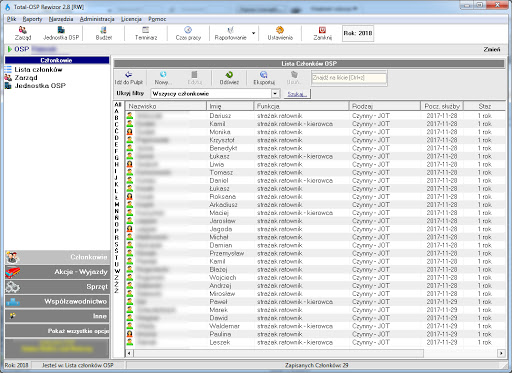
\includegraphics[width=\textwidth]{img/chapter2/total-osp.jpg}
    \caption{Interfejs użytkownika aplikacji TOTAL-OSP}
    \label{fig:TOTAL-OSP}
\end{figure}


Niestety interfejs aplikacji uchwycony na rys. \ref{fig:TOTAL-OSP} wygląda na bardzo przestarzały. Program został zaprojektowany na podobieństwo dawnego oprogramowania pakietów biurowych. Mimo sterylnego uporządkowania funkcjonalności, aplikacja zdaje się być nudnym i przytłaczającym narzędziem pracy.

Kolejną wadą rozwiązania, jest okoliczność, że z programu można korzystać jedynie na komputerach z zainstalowanym systemem operacyjnym z rodziny Microsoft Windows. Niweluje to możliwości wykorzystania narzędzia poprzez urządzenia mobilne, co czyni je o wiele mniej podręcznym, a przede wszystkim wolniejszym. Konsekwencją powyższych wad jest możliwość korzystania z aplikacji jedynie przy komputerze stacjonarnym znajdującym się w budynku jednostki OSP. 
Na plus, można wyróżnić możliwość instalacji oprogramowania na wielu komputerach w tej samej sieci LAN, w ramach jednej licencji oraz gotowy mechanizm tworzenia kopii zapasowych bazy danych. 


%%%%%%%%%%%%%%%%%%%%%%%%%%%%%%%%%%%%%%%%%%%%%%%%%%%%%%%%%%%%%%%%%%%%%%%%%%%%%%%%
\section{mOSP}
%%%%%%%%%%%%%%%%%%%%%%%%%%%%%%%%%%%%%%%%%%%%%%%%%%%%%%%%%%%%%%%%%%%%%%%%%%%%%%%%

Kolejne rozwiązanie zostało stworzone przez polską firmę MatSol. Według danych zamieszczonych na stronie produktu, w roku 2015 ponad 600 jednostek OSP wykorzystywało ich produkt, co świadczy o jego umiarkowanym sukcesie na rynku oprogramowania \cite{mOSP}.

mOSP jest konkurencyjną aplikacją, stworzoną w bardzo zbliżonym okresie do rozwiązania opisanego w sekcji 2.2. Poza mniej użytecznymi dodatkami, takimi jak moduł odpowiedzialny za organizację zawodów strażackich, posiada ona praktycznie te same funkcjonalności co TOTAL-OSP.

\begin{figure}
    \centering
    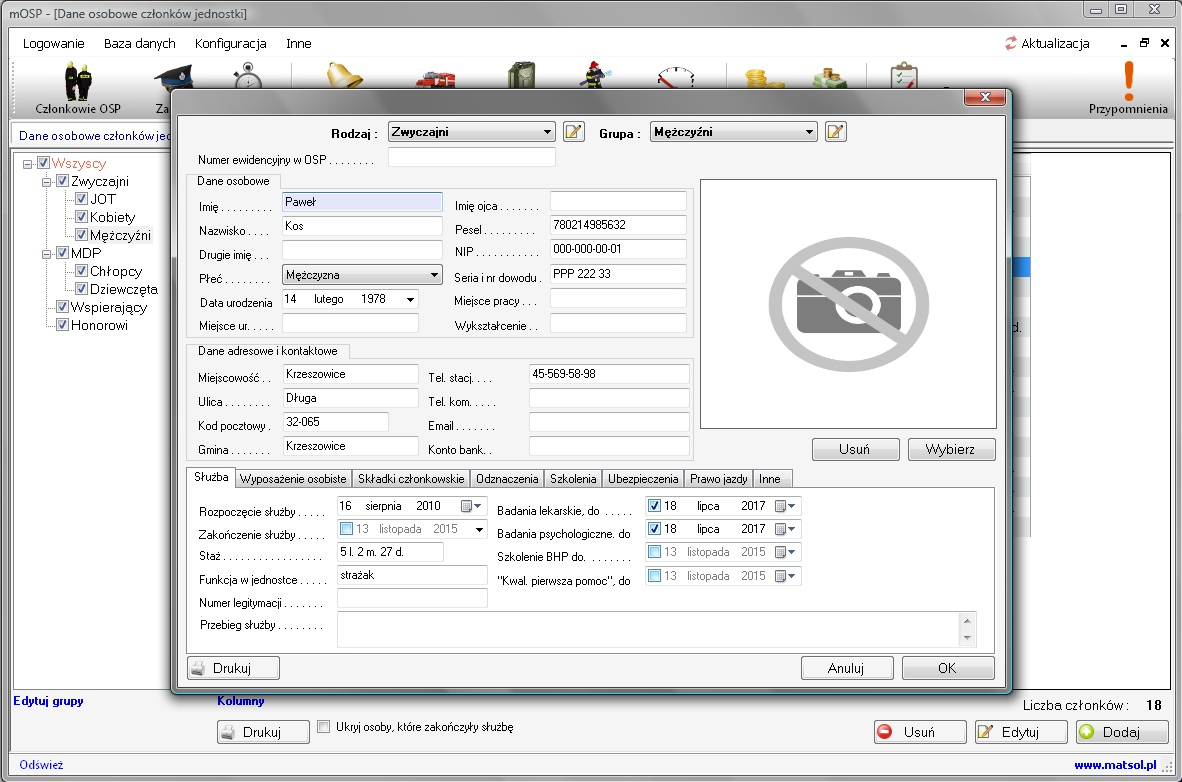
\includegraphics[width=\textwidth]{img/chapter2/m-osp.jpg}
    \caption{Interfejs użytkownika aplikacji mOSP}
    \label{fig:mOSP}
\end{figure}

Twórcy mOSP uczynili interfejs użytkownika programu podobnym do arkuszy kalkulacyjnych, w których najważniejszą rolę pełnią tabele (rys. \ref{fig:mOSP}). Zunifikowany interfejs odpłaca się bardziej intuicyjną obsługą oprogramowania. Niestety, mimo dużej sterylności widoków, program wydaje się być przestarzały i nieciekawy dla użytkownika.

Jedna licencja oprogramowania pozwala na skorzystanie z aplikacji na trzech komputerach, ale jedynie z systemem operacyjnym Windows. Analogicznie jak w przypadku opisanej powyżej aplikacji TOTAL-OSP brak jest możliwości wykorzystania narzędzia poprzez urządzenia mobilne do codziennej pracy w terenie. 

%%%%%%%%%%%%%%%%%%%%%%%%%%%%%%%%%%%%%%%%%%%%%%%%%%%%%%%%%%%%%%%%%%%%%%%%%%%%%%%%
\section{OSPiko}
%%%%%%%%%%%%%%%%%%%%%%%%%%%%%%%%%%%%%%%%%%%%%%%%%%%%%%%%%%%%%%%%%%%%%%%%%%%%%%%%

Ostatnim rozpatrywanym rozwiązaniem jest  OSPiko od przedsiębiorstwa TomPiko. Program zyskał uznanie wielu jednostek OSP, których opinie można przeczytać na stronie producenta \cite{OSPiko}.

OSPiko dubluje wszystkie najważniejsze funkcjonalności swoich poprzedników, rozbijając niektóre moduły na mniejsze. Każdy z modułów ewidencyjnych posiada również możliwość drukowania ujednoliconych i prostych raportów z działalności jednostki.

\begin{figure}
    \centering
    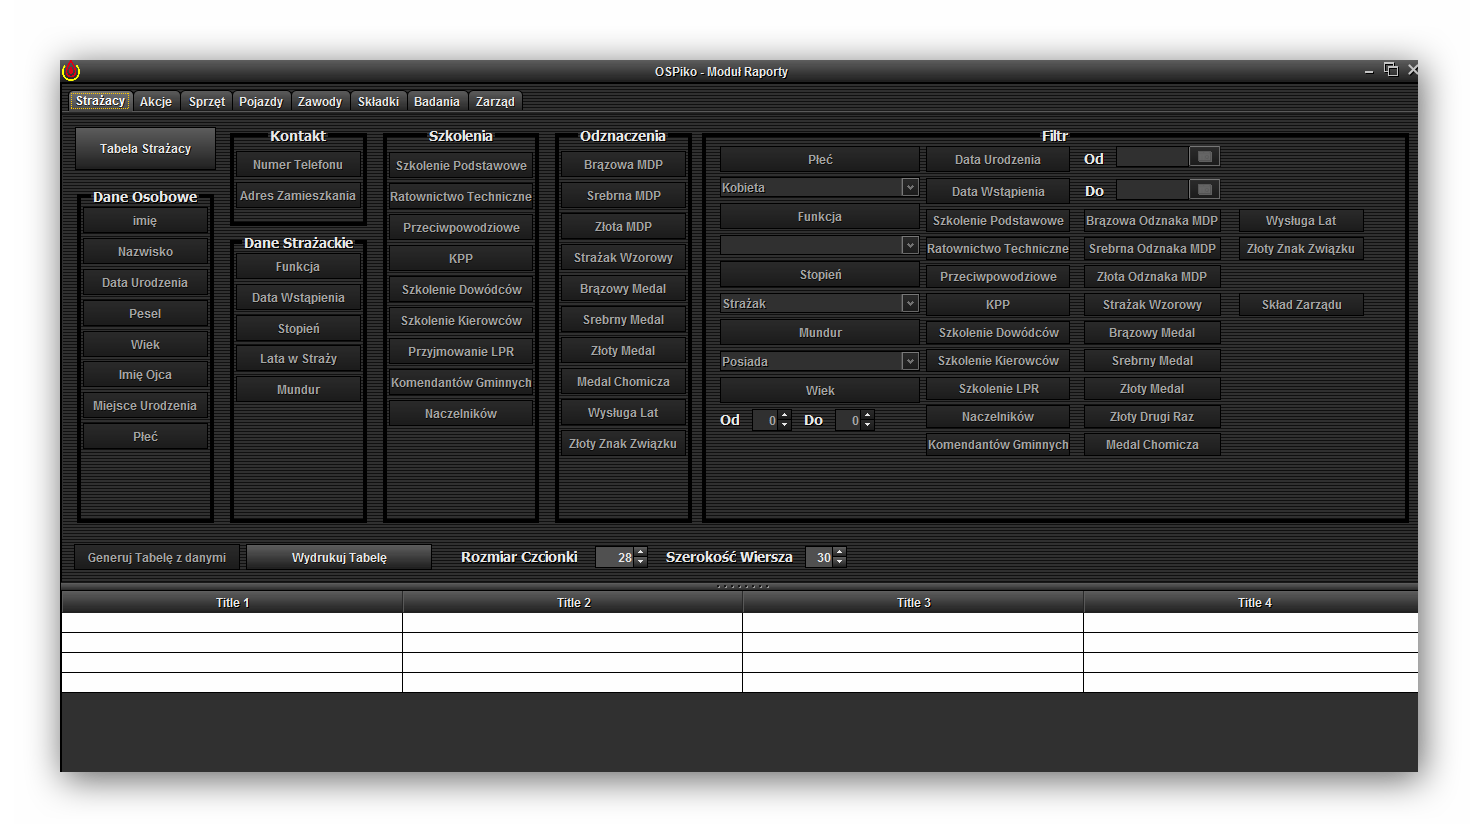
\includegraphics[width=\textwidth]{img/chapter2/ospiko.png}
    \caption{Interfejs użytkownika aplikacji OSPiko}
    \label{fig:OSPiko}
\end{figure}

Aplikacja wyróżnia się spośród pozostałych bardziej nowoczesnym interfejsem użytkownika i dobrą organizacją okien oraz formularzy (rys. \ref{fig:OSPiko}). Powyższe, czyni ją bardziej przyjazną użytkownikowi i sprawia, że korzystanie z niej wiąże się z większą satysfakcją.

Twórcy programu udostępniają możliwość kupna licencji przypisanej sprzętowo do jednego komputera lub wersji przenośnej, umożliwiającej korzystanie z oprogramowania na różnych stanowiskach, ale wyłącznie z zainstalowanym systemem operacyjnym Windows. Ogranicza to możliwość korzystania z aplikacji w terenie, podobnie jak w przypadku konkurencyjnych produktów.


%%%%%%%%%%%%%%%%%%%%%%%%%%%%%%%%%%%%%%%%%%%%%%%%%%%%%%%%%%%%%%%%%%%%%%%%%%%%%%%%
\section{Podsumowanie}
%%%%%%%%%%%%%%%%%%%%%%%%%%%%%%%%%%%%%%%%%%%%%%%%%%%%%%%%%%%%%%%%%%%%%%%%%%%%%%%%

Funkcjonujące na rynku, gotowe rozwiązania są bardzo funkcjonalnymi programami, które spełniają swoje zadania w dostatecznym stopniu. Niektóre z nich, poza prowadzeniem elektronicznego rejestru jednostki, udostępniają możliwość drukowania statystyk i dokumentów przydatnych w pracy OSP.

Jednakże, ich wspólną wadą pozostaje fakt uzależnienia od komputerów z systemem Windows oraz stosunkowo mało atrakcyjne interfejsy użytkownika. Zniechęca to część potencjalnych klientów oraz co gorsza uniemożliwia wykorzystanie popularnych urządzeń mobilnych. Rezygnacja z szybkiej interakcji z systemem, przy pomocy dostępnego pod ręką urządzenia, stanowi poważny problem. Rozwiązanie tego problemu stanowi kluczowy element niniejszej pracy.


\chapter{Teoretyczne podstawy systemów internetowych}
%%%%%%%%%%%%%%%%%%%%%%%%%%%%%%%%%%%%%%%%%%%%%%%%%%%%%%%%%%%%%%%%%%%%%%%%%%%%%%%%
\section{Krótka geneza Internetu}
%%%%%%%%%%%%%%%%%%%%%%%%%%%%%%%%%%%%%%%%%%%%%%%%%%%%%%%%%%%%%%%%%%%%%%%%%%%%%%%%

Za początek pracy, nad powszechnie znanymi dziś technologiami internetowymi, uznaje się lata 60-te XX wieku. Wówczas, wybitni przedstawiciele środowisk informatycznych, rozpoczęli pracę nad nowym sposobem przesyłu danych ,zwanym komutacją pakietów.

Wedle udokumentowanej w literaturze historii Internetu \cite{Leiner.history-of-internet}, istniały aż trzy niezależne od siebie źródła pracy nad ideą komutacji pakietów: 

\begin{itemize}
    \item Działalność akademicka naukowców z MIT (Massachusetts Institute of Technology) w Stanach Zjednoczonych. Opracowana przez nich teoria, została wykorzystana do stworzenia pierwszego na świecie prototypu rozległej sieci komputerowej (WAN) przy pomocy sieci telefonicznej.
    \item Badania naukowe NPL (National Physical Laboratory) w Anglii, w których po raz pierwszy użyto terminu "pakiet" wobec jednostek danych.
    \item Projekt niezawodnego systemu komunikacji dla armii Stanów Zjednoczonych, stworzony przez działaczy organizacji badawczej RAND (Research And Development), z udziałem Paula Barana \cite{Baran.komutacja-pakietow}.
\end{itemize}

Wyniki pracy każdego z zespołów, przełożyły się na projekt rewolucyjnej sieci ARPANET, tworzonej pod patronatem amerykańskiej organizacji DARPA (Defense Advanced Research Projects Agency). Z początku łączyła ona jedynie Uniwersytet Kalifornijski i ośrodek naukowy SRI (Stanford Research Institute). W roku 1968 przeprowadzona została pierwsza pomyślna transmisja host-to-host między tymi węzłami. 

ARPANET, w kolejnych latach, został rozbudowany o wiele nowych węzłów, osadzonych głównie w akademickich placówkach badawczych, pozostając wciąż tajemnicą dla opinii publicznej. Zdecydowanym krokiem naprzód, było ostateczne dopracowanie protokołu NCP (Network Control Program), ściśle określającego przebieg przesyłu pakietów za pośrednictwem urządzeń IMP (Interface Message Processor). Same urządzenia IMP stanowiły pierwszą generację urządzeń, zwanych bramami sieciowymi, stanowiących mediator między komunikującymi się przez ARPANET komputerami (hostami), podłączonymi do dwóch różnych sieci lokalnych (LAN). Umożliwiło to stworzenie, pierwszych znaczących aplikacji do przesyłu plików i komunikatów, między hostami tworzonej sieci WAN.

ARPANET, po raz pierwszy został zaprezentowany publicznie w 1972 roku na konferencji ICCC (International Computer Communication Conference), spotykając się z entuzjastycznym odbiorem. W tym samym roku, przedsiębiorstwo BBN Technologies, utworzyło oprogramowanie umożliwiające skorzystanie z pierwszej w historii sieci email, za pośrednictwem sieci ARPANET, dokonując przełomu w metodach komunikacji międzyludzkiej.

Ewolucja sieci ARPANET, w znany dzisiaj powszechnie Internet, była wynikiem wielu zmian i ogromnego nakładu pracy wizjonerów, którzy kształtowali nowy porządek w dziedzinie sieci komputerowych. Szczegółowe opisanie każdego z etapów tego procesu, znacznie wykracza poza zakres tworzonej pracy. Poniżej przedstawiono wyłącznie najważniejsze nurty kształtujące dzisiejszy Internet:

\begin{itemize}
    \item Pierwotni architekci sieci ARPANET, zdecydowali się na obranie nowej strategii, polegającej na tworzeniu sieci, zgodnie z zasadą otwartej architektury. Regułą stało się opracowywanie ogólnodostępnych standardów i specyfikacji, umożliwiających twórcom oprogramowania i sprzętu komputerowego, tworzenie kompatybilnych ze sobą rozwiązań, mogących w pełni wykorzystywać możliwości sieci Internet. Wspomniane dokumenty od 1969 roku, są publikowane i komentowane w ramach zbioru Request for Comments (RFC) \cite{RFC.index}. Dużą rolę w rozpowszechnianiu i rozwoju tych standardów, odgrywa organizacja Internet Engineering Task Force (IETF).
    \item Protokół NPC wraz z urządzeniami IMP ze względu na swoje ograniczenia, zostały zastąpione przez nowsze odpowiedniki - protokół TCP/IP oraz współpracujące z nimi nowe generacje bram sieciowych. Z początku protokół kontroli transmisji (TCP) oraz protokół internetowy (IP) stanowiły jedną nierozłączną całość, by następnie zostać rozdzielone na dwie niezależne od siebie specyfikacje.
    \item We wrześniu 1981 roku, opublikowana została specyfikacja RFC 791, stanowiąca opis czwartej wersji protokołu IP \cite{RFC.791.IP}, która do dziś jest dominującym standardem identyfikowania komputerów w internecie.
    \item Ostateczne zaprzestanie eksploatacji protokołu NPC na rzecz stosu TCP/IP zostało zaplanowane na 1 stycznia 1983 roku i przebiegło zaskakująco pomyślnie. Dzięki tej ważnej zmianie, w drugiej połowie lat 80-tych XX wieku, na rynku zaczęły pojawiać się pierwsze oferty komercyjnych dostawców usług internetowych (ISP).
\end{itemize}

Mimo prężnego rozwoju technologii internetowych, u podstaw ich działania wciąż leży idea komutacji pakietów. Zgodnie z jej metodologią, przesyłany strumień danych musi zostać podzielony na mniejsze jednostki zwane pakietami. Każdy pakiet zawiera porcje danych oraz swój nagłówek wykorzystywany do jego identyfikacji. Tak przygotowane pakiety przesyłane są przez węzły sieci, podlegając niezależnemu od innych pakietów trasowaniu (tj. wyboru kolejnych węzłów, przez które zostaną przesłane do odbiorcy).

%%%%%%%%%%%%%%%%%%%%%%%%%%%%%%%%%%%%%%%%%%%%%%%%%%%%%%%%%%%%%%%%%%%%%%%%%%%%%%%%
\section{Epoka World-Wide Web}
%%%%%%%%%%%%%%%%%%%%%%%%%%%%%%%%%%%%%%%%%%%%%%%%%%%%%%%%%%%%%%%%%%%%%%%%%%%%%%%%

W końcówce lat 80-tych XX wieku, Internet, na przekór swoim ogromnym możliwościom, wciąż pozostawał mało wygodnym narzędziem, zarówno dla twórców oprogramowania jak i użytkowników przeszukujących sieć w celu uzyskania informacji. W następstwie tego, w 1989 roku, Tim Berners-Lee, informatyk pochodzenia brytyjskiego, rozpoczął pracę nad projektem WorldWideWeb (WWW lub W3) \cite{Berners-Lee.world-wide-web}. Projekt zakładał opracowanie prostszej i przystępniejszej metody wykorzystania sieci internetowej.

Założeniem nowego sposobu eksploracji zasobów, udostępnionych za pośrednictwem Internetu, było przenoszenie się po zawartości plików hipertekstowych przy pomocy umieszczonych w nich odnośników (linków). Koncepcja WWW korzystała z architektury klient-serwer, w której zadaniem klienta było przetwarzanie kompleksowej warstwy prezentacji, a zadaniem serwerów wydajne przeszukiwanie i manipulacja danymi.

By osiągnąć zamierzony efekt, opracowano nowy protokół HTTP (Hypertext Transfer Protocol), służący komunikacji klienta z serwerem. Zapewniał on nowe funkcjonalności, takie jak uzyskiwanie plików tekstowych po ich nazwie, czy przeszukiwanie spisu dokumentów po frazie podanej przez użytkownika, przy użyciu pojedynczych połączeń TCP/IP. Protokół ten do dziś, stanowi główny sposób wykorzystywania usług internetowych przez ich użytkowników, wraz z jego wersją HTTPS dodającą możliwość szyfrowania wysyłanych żądań. 

Dużą rolę w działaniu sieci WWW, odgrywają unikatowe identyfikatory zasobów URI. Specyfikacja ta umożliwia identyfikacje zasobów udostępnionych w ramach serwerów HTTP przy pomocy ciągu znaków. Identyfikatory najczęściej kojarzone są ze ścieżkami do pojedynczych plików, znanych z systemów operacyjnych. Pierwotnie URI zostały opracowane w dokumencie RFC 2396 przez Bernersa-Lee oraz jego współpracowników. Jednakże podobnie jak inne internetowe standardy, podlegają rewizji w nowszych dokumentach z tej serii \cite{rfc.2396.URI}.

Kluczowym narzędziem w technologiach WWW, jest oprogramowanie znane jako przeglądarki internetowe. Głównych zadaniem tych programów jest wysyłanie i odbiór żądań HTTP oraz odpowiedzi na te żądania. Dodatkowo, pełnią one rolę interpretera odbieranych plików hipertekstowych, wyświetlając wygenerowany na ich podstawie tekst, odnośniki, multimedia oraz elementy interfejsu użytkownika.

We wrześniu 1990 roku, Tim Berners-Lee stworzył pierwszy w historii serwer HTTP o nazwie httpd oraz narzędzie klienckie WorldWideWeb. Było ono, jednocześnie przeglądarką internetową, jak i edytorem plików hipertekstowych. Stworzony prototyp został pozytywnie przyjęty przez użytkowników, a WWW zaczęło zyskiwać coraz większą rzeszę zwolenników.

W 1994 roku, Berners-Lee założył organizację World Wide Web Consortium (W3C), zrzeszającą zwolenników sieci WWW. Jej główną misją jest promowanie i rozwój technologii W3, poprzez tworzenie i ulepszanie rządzących nią protokołów oraz specyfikacji. Umożliwia to produktywne tworzenie i aktualizowanie przeglądarek internetowych przez niezależnych twórców oraz łatwy rozwój aplikacji internetowych. Dzięki temu, sieć WWW jest obecnie najpopularniejszym na świecie sposobem eksploatacji Internetu, a standardy z nią związane, potocznie nazywane są "technologiami webowymi" \cite{W3C.about}.

%%%%%%%%%%%%%%%%%%%%%%%%%%%%%%%%%%%%%%%%%%%%%%%%%%%%%%%%%%%%%%%%%%%%%%%%%%%%%%%%
\section{Hipertekstowy język znaczników HTML}
%%%%%%%%%%%%%%%%%%%%%%%%%%%%%%%%%%%%%%%%%%%%%%%%%%%%%%%%%%%%%%%%%%%%%%%%%%%%%%%%

Podstawą działania stron internetowych WWW są dokumenty hipertekstowe. Na potrzeby przetestowania swojej nowej koncepcji, twórca WorldWideWeb sformułował pierwszą specyfikację hipertekstowego języka znaczników (HTML) w 1990 roku. Jednakże, nie traktowano jej jako oficjalnego standardu. Dopiero w 1993 roku, członkowie organizacji IETF, rozpoczęli tworzenie wersji roboczej oficjalnej specyfikacji, ostatecznie dokończonej z ramienia W3C w 1995 roku. Standardowi, stworzonemu dla użytkowników Internetu, nadano nazwę HTML 2.0 \cite{RFC.1866.HTML-2}. 

W końcówce lat 90-tych XX wieku, standard HTML otrzymał jeszcze kilka rewizji, rozbudowujących go o nowe funkcjonalności, kończąc na wersji HTML 4.01 w 1999 roku. W maju 2000 roku, międzynarodowa organizacja normalizacyjna (ISO) utworzyła standard ISO/IEC 15445:2000, hipertekstowego języka znaczników bazujący bezpośrednio na HTML 4.01 \cite{ISO.HTML}.

Przez ponad dekadę, specyfikacja HTML nie podlegała większym zmianom, aż do 2014 roku. Wtedy to, opublikowana została wersja HTML 5.0 kompleksowo przekształcająca możliwości dokumentów hipertekstowych i wprowadzająca wiele nowych znaczników. Decydujący wpływ na rozwój piątej wersji języka HTML, miała założona specjalnie w tym celu grupa Web Hypertext Application Technology Working Group (WHATWG). 

Podczas gdy organizacja W3C zajęta była rozwojem nowego standardu XHTML, grupa WHATWG tworzyła rozwiązanie kompatybilne ze starszymi wersjami języka HTML. Niektóre nowości ze standardu XHTML 1 stały się również elementami HTML5.  Grupa WHATWG jest obecnie częścią W3C odpowiedzialną za aktualizowanie standardu w jego podwersjach. Spekuluje się, że HTML5 zostanie rekomendowaną wersją, jeszcze przez co najmniej kilka następnych lat, będąc rozwijanym jako żywy standard, otrzymujący częste aktualizacje i uzupełnienia \cite{html.whatwg}.

Dokumenty napisane w hipertekstowym języku znaczników, są plikami tekstowymi zawierającymi znaczniki występujące w nawiasach ostrych np. <html>, <div> czy <img>. Najczęściej znaczniki te, występują w parach - pierwszy ze znaczników nazywany jest znacznikiem początkowym (otwierającym), a drugi znacznikiem końcowym (zamknięcia). Dodatkowo, znacznik końcowy odróżnia znak "/" przed jego nazwą np. otwierający <html> i zamykający </html>. W języku HTML wyróżniamy również znaczniki pojedyncze jak np. <img>, reprezentujący obraz cyfrowy występujący na stronie. 

Jako dodatkowy opis elementu reprezentowanego przez znacznik, wykorzystuje się tzw. atrybuty. Atrybuty to wartości opisane przez łańcuch znaków, przypisane do odpowiednich nazw wewnątrz nawiasów <> znacznika rozpoczynającego. Mogą one występować w dowolnej kolejności, jednakże zawsze po nazwie opisywanego znacznika. Należy również zaznaczyć fakt, że w rozpoznawaniu nazw znaczników i ich atrybutów, nie występuje rozróżnienie na małe i duże litery tj. <HTML> jest równoznacznym znacznikiem z <html>.

\begin{lstlisting}[language=HTML, caption=Przykładowy dokument HTML5, label=lst:html.example]
    <!DOCTYPE html>
    <html lang="pl">
    	<head>
            <meta http-equiv="content-type" content="text/html" charset="utf-8">
            <meta http-equiv="content-language" content="pl">
            <title>Tytuł tej strony</title>
    	</head>
    	<body>
            <header>
                <img src="https://via.placeholder.com/200x150?text=LOGO_STRONY">
                <h1>Tytuł strony</h1>
            </header>
            <nav>
                <ul>
                    <li><a href="home.html">Strona główna</a></li>
                    <li><a href="forum.html">Forum</a></li>
                    <li><a href="about.html">O nas</a></li>
                    <li><a href="contact.html">Kontakt</a></li>
                <ul>
            </nav>
            
            <section>
                <h2>Sekcje dzielą główną treść strony na części</h2>
                <article>
                    <h4>Dodatkowy podział sekcji na artykuły</h4>
                    <p>Każda sekcja może zostać dodatkowo podzielona na artykuły
                    takie jak ten.</p>
                </article>
                <article>
                    <h4>Warto korzystać z nowych znaczników HTML5</h4>
                    <p>Mimo, że nie jest to wymagane, korzystne jest zastosowanie 
                    nowej konwencji w swoich projektach.</p>
                </article>
            </section>
            
            <aside>
                <img src="https://via.placeholder.com/120x240?text=Reklama">
            </aside>
            
            <footer>
                <img src="https://via.placeholder.com/100x75?text=LOGO_W_STOPCE">
                <p>Strona testowa 2021</p>
            </footer>
        </body>
    </html>
\end{lstlisting}

Na listingu \ref{lst:html.example} przedstawiony został przykładowy plik HTML. Zgodnie z zaleceniami W3C, dokumenty publikowane w internecie rozpoczynają się od deklaracji ich typu, aby przeglądarka internetowa otrzymała informacje jaki plik przetwarza. Pliki HTML5 rozpoczynają się od linii <!DOCTYPE html>. Następnie otwierany jest znacznik <html> wyznaczający granice dokumentu hipertekstowego.

Wewnątrz znacznika <html> zagnieżdżone zostały dwa kolejne. Znacznik <head> pełni funkcję nagłówka strony poświęconemu jej metadanym. Metadane, wykorzystywane są, aby zapewnić przeglądarce internetowej oraz oprogramowaniu przeszukującemu Internet, dodatkowe informacje przyczyniające się do poprawnego zinterpretowania treści dokumentu. Przykładowo zostały przedstawione trzy znaczniki metadanych:

\begin{itemize}
    \item Pierwszy znacznik <meta>, zawiera atrybuty określające sposób kodowania pliku. Dzięki temu znaki specjalne zostaną wyświetlone w przeglądarce w prawidłowy sposób.
    \item Atrybuty drugiego znacznika <meta> określają język w jakim napisany jest dokument. Informacja ta może zostać wykorzystana do automatycznego tłumaczenia strony przy pomocy dodatkowego oprogramowania.
    \item Ostatni znacznik <title> definiuje nazwę strony, która zostanie wyświetlona w opisie karty w przeglądarce internetowej.
\end{itemize}

Kolejnym znacznikiem zagnieżdżonym w <html> jest <body>. W jego wnętrzu, zdefiniowane jest całe ciało strony, czyli wszystkie elementy, widoczne w obrębie okna przeglądarki. Przestrzegając reguł narzuconych przez specyfikacje języka, twórcy dokumentu są w stanie modelować wyświetlaną strukturę elementów, w dowolny sposób. Standard HTML5 wprowadził jednak zbiór znaczników semantycznych, ułatwiających tworzenie struktury, przejrzystej zarówno dla użytkowników przeglądających Internet, jak i dla innych programistów czytających kod źródłowy strony.

\begin{figure}[!htbp] 
    \centering
    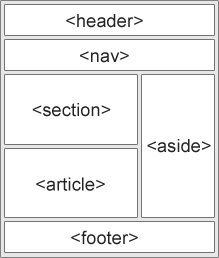
\includegraphics{img/chapter3/html.semantic-elements.png}
    \caption{Przykładowy diagram struktury elementów semantycznych z oficjalnej strony W3C}
    \label{fig:html.semantic-elements}
\end{figure}

Znaczniki semantyczne to takie, których nazwa wskazuje na przetrzymywaną w nich zawartość. Pierwszym elementem w proponowanej na rys. \ref{fig:html.semantic-elements} strukturze jest <header>. Zgodnie z nazwą, jest to nagłówek strony, w którym powinny zostać umieszczone elementy takie jak logo, tytuł lub motto. Następny to <nav> reprezentujący elementy nawigacyjne, takie jak wysuwany boczny panel lub horyzontalną belkę, zawierające odnośniki do stron tworzących najważniejsze sekcje portalu internetowego. Linki zagnieżdżone w elemencie <nav> rozpoznawane są przez nowoczesne wyszukiwarki internetowe, jako podelementy strony głównej portalu, ułatwiając szybki dostęp do wybranych treści.

Następne dwa popularne znaczniki to <section> oraz <article>. Najczęściej wykorzystuje się je do podziału głównej treści danej strony na pomniejsze części. Innym znacznikiem semantycznym o podobnym przeznaczeniu jest <main> wykorzystywany do okalania całej treści głównej, tak jak robi to <header> z nagłówkiem. Element <aside> użyty został do okalania zawartości znajdującej się na bok od treści głównej. W przykładowym listingu \ref{lst:html.example} jest to wertykalny baner reklamowy. 

Strukturę strony kończy stopka, zawarta w elemencie <footer>. Stopka zwyczajowo używana jest do wyświetlenia informacji o twórcach strony oraz latach w których rozwijano portal. Czasami zawiera alternatywne linki nawigacyjne oraz gwarantuje szybki dostęp do informacji kontaktowych \cite{Mazur.html5-css3}.

\begin{figure}[!htbp] 
    \centering
    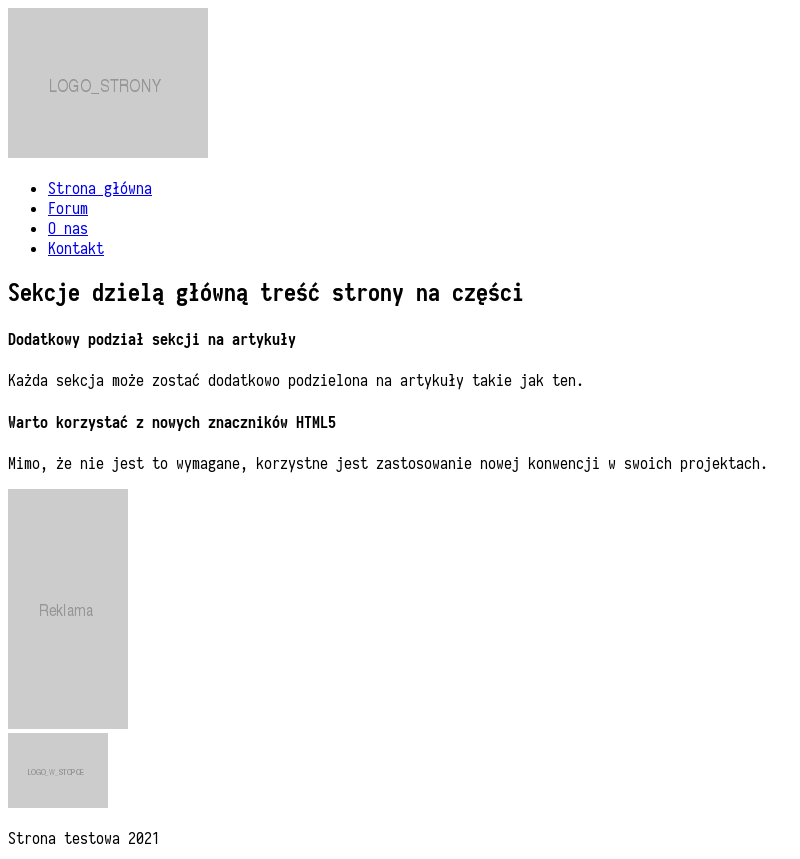
\includegraphics[width=\textwidth]{img/chapter3/html.example.rendered.png}
    \caption{Przykładowa strona wyświetlona przez przeglądarkę na podstawie dokumentu z listingu \ref{lst:html.example}}
    \label{fig:html.example.rendered}
\end{figure}

Na rys. \ref{fig:html.example.rendered} przedstawiona została strona internetowa wyświetlona przez przeglądarkę na podstawie listingu \ref{lst:html.example}. Mimo nie najgorszej przejrzystości wyświetlanej treści, strona nie wygląda szczególnie ciekawie czy oryginalnie. Język HTML został wzbogacony o znaczniki i atrybuty, umożliwiające w ograniczonym stopniu modyfikację wyglądu wyświetlanych elementów. Nie są one jednak dobrym narzędziem do osiągnięcia tego celu. Aby efektywnie zapobiec monotonii stron internetowych, opracowane zostały kaskadowe arkusze stylów, opisane w następnej sekcji.

%%%%%%%%%%%%%%%%%%%%%%%%%%%%%%%%%%%%%%%%%%%%%%%%%%%%%%%%%%%%%%%%%%%%%%%%%%%%%%%%
\section{Kaskadowe arkusze stylów CSS}
%%%%%%%%%%%%%%%%%%%%%%%%%%%%%%%%%%%%%%%%%%%%%%%%%%%%%%%%%%%%%%%%%%%%%%%%%%%%%%%%

W 1994 roku, działacze W3C pracujący nad językiem HTML, rozważyli propozycję stworzenia kaskadowych arkuszy stylów (CSS), których zadaniem byłoby uproszczenie procesu stylizacji stron internetowych. Jako efekty tych prac, wyróżnia się rekomendację CSS1 (1996) oraz uzupełniającą ją CSS2 (1998). Od 2004 do 2011 roku, rozwijana była specyfikacja CSS2.1. Jednakże, w 2011 roku, podjęta została decyzja o podziale specyfikacji kaskadowych arkuszy stylów na pomniejsze, rozwijane niezależnie od siebie moduły.

W tym samym roku, udostępnione zostały moduły selektorów, kolorów i przestrzeni nazw poziomu trzeciego, bazujące na wersjach CSS2.1, a rekomendowaną specyfikacją stał się CSS3. Większość modułów CSS3, osiągnęła już trzeci poziom swojego rozwoju, ale nowe zaczynają rozwój od poziomu pierwszego, jak na przykład popularny moduł Flexbox, opublikowany w 2017 roku. Istnieją już moduły na poziomie 4, co zapowiada możliwą zmianę rekomendowanego standardu na CSS4 w najbliższej dekadzie. 

Arkusz CSS, stworzony jest z reguł, opisujących style elementów dokumentu hipertekstowego. Każda reguła składa się z selektora i deklaracji. Selektory są wskaźnikami na elementy, które powinny zostać ustylizowane przez daną regułę. Najczęściej selektorami są znaczniki elementów z dokumentu HTML. Deklaracja zawiera natomiast właściwości oraz przypisane im wartości.

Kaskadowość arkuszy CSS, polega na hierarchii ważności poszczególnych stylów, opisanych przy ich pomocy. Tworząc je, należy pamiętać o wyższym priorytecie bardziej szczegółowych selektorów, np. selektor wskazujący na elementy listy ma pierwszeństwo nad wskazującym na listę jako całość. Ponadto, arkusze stylów wystąpić mogą w jednej z trzech opisanych poniżej form:

\begin{itemize}
    \item Style lokalne - sformułowane jako atrybuty konkretnego elementu HTML. Każdy element HTML może posiadać atrybut "style" wewnątrz którego, znajdą się stylizujące go deklaracje. Niektóre elementy posiadają unikalne atrybuty tworzące deklaracje stylizujące np. element <img> posiada atrybuty "width" i "height" pozwalające zadeklarować szerokość i wysokość wyświetlanego obrazka.
    \item Wewnętrzny arkusz stylów występujący w nagłówku pliku hipertekstowego. Arkusz wewnętrzny zagnieżdżony jest w specjalnym elemencie <style>.
    \item Zewnętrzny plik CSS - dołączany do pliku hipertekstowego w jego nagłówku. Dodatkową korzyścią z zastosowania tej metody jest możliwość uwzględnienia  arkusza stylów z wielu plików jednocześnie.
\end{itemize}

W celu zaprezentowania każdej z trzech metod, na listingach  \ref{lst:css.local-style-example} oraz \ref{lst:css.head-style-example} przedstawione zostały zmodyfikowane fragmenty pliku HTML z listingu \ref{lst:html.example}.

\begin{lstlisting}[language=HTML, caption=Przykład stylu lokalnego CSS w dokumencie HTML, label=lst:css.local-style-example]
<nav>
    <ul>
      <li><a href="index.html" style="color: #f6f7eb;"><div>Strona główna</div></a></li>
      <li><a href="forum.html"><div>Forum</div></a></li>
      <li><a href="about.html"><div>O nas</div></a></li>
      <li><a href="contact.html"><div>Kontakt</div></a></li>
    </ul>
</nav>
\end{lstlisting}

Najwyższy priorytet posiadają selektory określone jako styl lokalny dla wybranego elementu HTML. Na listingu \ref{lst:css.local-style-example} jako przykład, zastosowano styl określający kolor czcionki, na biały,  dla odnośnika wskazującego na obecnie przeglądaną stronę (plik index.html).

\begin{lstlisting}[language=HTML, caption=Przykład stylów CSS zastosowanych przy pomocy nagłówka dokumentu HTML, label=lst:css.head-style-example]
<head>
  <meta http-equiv="content-type" content="text/html" charset="utf-8">
  <meta http-equiv="content-language" content="pl">
  <title>Tytuł tej strony</title>
  <link rel="stylesheet" href="node_modules/normalize.css/normalize.css" type="text/css">
  <style type="text/css">
    body {
      margin: 0;
      padding: 0;
      color: #f6f7eb;
      background-color: #5c414d;
      font-family: 'Akaya Kanadaka', sans-serif;
    }
  </style>
  <link rel="stylesheet" href="css/small.css" type="text/css">
  <link rel="stylesheet" href="css/medium.css" type="text/css">
  <link rel="stylesheet" href="css/large.css" type="text/css">
</head>
\end{lstlisting}

Listing \ref{lst:css.head-style-example} rozbudowuje nagłówek strony o element <style> w obrębie którego, można dowolnie definiować selektory CSS. Dołączanie zewnętrznych arkuszy CSS, realizowane jest przy pomocy elementów <link> z atrybutami definiującymi typ i ścieżkę do pliku.

\begin{lstlisting}[language=HTML, caption=Fragment pliku small.css załączonego w nagłówku dokumentu HTML, label=lst:css.example.small]
nav>ul>li>a {
  color: #cf8e80;
  text-decoration: none;
  font-size: larger;
}

nav>ul>li>a>div {
  padding: 0.4em 2em;
  text-align: center;
}

nav>ul>li>a>div:hover {
  background-color: #f6f7eb42;
}

main {
  padding: 1.5em;
  background-color: #f6f7eb10;
  display: grid;
  grid: auto-flow min-content / 1fr;
  grid-gap: 2em;
  justify-items: center;
}

section {
  display: grid;
  grid: auto-flow min-content / 1fr;
  grid-gap: 0.6em
}

article>h4, footer>p {
  color: #cf8e80;
}

#commercial-vertical {
  display: none;
}

#commercial-horizontal {
  display: block;
}
\end{lstlisting}

\begin{figure}[!htbp] 
    \centering
    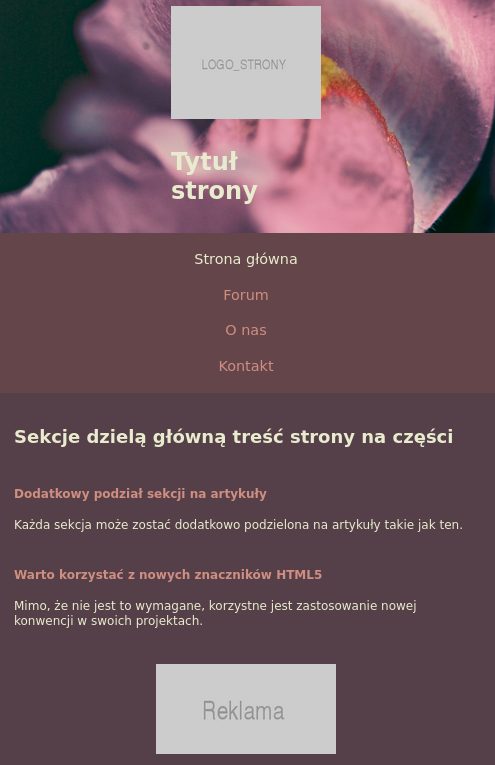
\includegraphics[width=\textwidth]{img/chapter3/css.example.small.png}
    \caption{Przykładowa strona z listingu \ref{lst:html.example} po zastosowaniu kaskadowych arkuszy stylów}
    \label{fig:css.example.small}
\end{figure}


Priorytet deklaracji stylów określonych w załączonych plikach oraz elemencie <style> określa kolejność występowania w nagłówku. Przy każdym wystąpieniu tego samego selektora, dodaje się deklaracje niezdefiniowane wcześniej oraz nadpisuje się wartości tych, które zostały już użyte.

Obecnie jednym z najważniejszych zastosowań kaskadowych arkuszy stylów, jest dostosowywanie sposobu wyświetlania treści na stronie do rozdzielczości ekranu.  Jest to możliwe dzięki nowym zapytaniom typu media poziomu 3. Cecha ta jest nazywana potocznie responsywnością aplikacji.
Dla HTML4 oraz CSS2 w specyfikacji istniało już słowo kluczowe "media"  pozwalające dostosować wyświetlaną treść do określonego typu dokumentu tj. strona internetowa czy dokument do wydruku. Poziom 3, umożliwił natomiast dostosowywanie deklaracji CSS do parametrów wyświetlania dokumentu, takich jak szerokość oraz wysokość, aspekt czy orientacja strony wyświetlanej na urządzeniu \cite{css.media-queries}.

\begin{lstlisting}[language=CSS, caption=Plik medium.css załączony w nagłówku dokumentu HTML, label=lst:css.example.medium]
@media only screen and (min-width: 720px) {
  header {
    grid: min-content max-content / min-content min-content; 
    align-items: center;
  }
    
  main {
    grid: auto-flow min-content / 1fr min-content;
    align-items: center;
  }

  #commercial-vertical {
    display: block;
  }

  #commercial-horizontal {
    display: none;
  }
}
\end{lstlisting}

\begin{lstlisting}[language=CSS, caption=Plik large.css załączony w nagłówku dokumentu HTML, label=lst:css.example.large]
@media only screen and (min-width: 1024px) {
  nav>ul {
    grid: auto-flow min-content / 1fr 1fr 1fr 1fr;
  }
}
\end{lstlisting}

Przykładowo na listingach \ref{lst:css.example.medium} oraz \ref{lst:css.example.large} przedstawiono zapytanie media w plikach medium.css i large.css. Podmieniają one deklaracje dotyczące sposobu wyświetlania elementów na stronie, na ekranach, których szerokość wynosi kolejno przynajmniej 720 i 1024 pikseli.

\begin{figure}[!htbp] 
    \centering
    
\includegraphics[width=\textwidth]{img/chapter3/css.example.medium.png}
    \caption{Przykładowa strona internetowa dla ekranów o szerokości większej niż 1024 pikseli}
    \label{fig:css.example.medium}
\end{figure}

Rzeczywiste zmiany sposobu wyświetlania strony względem rys. \ref{fig:css.example.small} można zaobserwować na rys. \ref{fig:css.example.medium}. Dzięki zastosowaniu kwerend media w ten sposób, zmiany zostały wprowadzone przyrostowo. Linki w nagłówku strony ułożono w sposób bardziej horyzontalny, a obrazek reprezentujący reklamę przesunięto na boczny panel strony.

%%%%%%%%%%%%%%%%%%%%%%%%%%%%%%%%%%%%%%%%%%%%%%%%%%%%%%%%%%%%%%%%%%%%%%%%%%%%%%%%
\section{JavaScript i model obiektowy dokumentu}
%%%%%%%%%%%%%%%%%%%%%%%%%%%%%%%%%%%%%%%%%%%%%%%%%%%%%%%%%%%%%%%%%%%%%%%%%%%%%%%%

Za pomocą opisanych w poprzednich sekcjach standardów HTML oraz CSS jesteśmy w stanie tworzyć dobrze przemyślane, atrakcyjne wizualnie i responsywne interfejsy użytkownika. Jednakże szybko okazuje się, że strony internetowe bazujące jedynie na tych dwóch technologiach, stanowią bardzo sztywne, praktycznie statyczne treści.

Dzięki funkcjonalnościom selektorów i deklaracji CSS poziomu trzeciego, jesteśmy w stanie definiować proste animacje do odegrania na elementach HTML, czy nawet odpowiedzi na interakcje, takie jak przykrycie kursorem powierzchni elementu. Wciąż jednak okazuje się, że te rozwiązania obarczone są dużymi ograniczeniami i wymagają dużej wprawy przy tworzeniu złożonych elementów interaktywnych.

Na potrzebę łatwiejszej implementacji elementów interaktywnych, jako pierwsi spróbowali odpowiedzieć pracownicy firmy Netscape Communications. Po ogromnym sukcesie ich przeglądarki Netscape Navigator w latach 90-tych XX wieku, początkowo zakładali oni zastosowanie jednego z popularnych wówczas języków programowania takich jak Java, Perl czy Python. Ostatecznie podjęto decyzję o zaimplementowaniu zupełnie nowego języka skryptowego na potrzeby programu Netscape Navigator 2.

W 1995 roku, Brendan Eich, rozpoczął pracę nad technologią nazwaną początkowo Mocha. Podczas dystrybucji wersji beta nowej przeglądarki, nazwę języka zmieniono początkowo na LiveScript , by następnie przemianować ją na znany do dziś JavaScript (JS).

W wyniku pozytywnego przyjęcia wersji JS 1.0, zarząd firmy Microsoft zadecydował o stworzeniu własnej, konkurencyjnej implementacji języka o nazwie JScript. Został on dołączony do przeglądarki Internet Explorer 3 w okresie zbliżonym do daty wydania programu Netscape Navigator 3, wyposażonego w nowe funkcjonalności JS 1.1. Niestety technologie te nie były ze sobą w pełni kompatybilne, zmuszając twórców aplikacji do tworzenia kilku wersji swoich produktów, w celu dostarczenia ich do większej rzeszy użytkowników.

Z uwagi na powyższe, w 1997 roku, firma Netscape zadecydowała o utworzeniu powszechnie dostępnego standardu ECMA-262 z pomocą instytucji ECMA International. ECMA jako organizacja powołana w celu ustanawiania oraz dystrybucji nowych norm w dziedzinie komunikacji i przetwarzania informacji, do dziś stanowi rzetelne źródło informacji o standardzie JavaScript.

Dzięki pracy fundacji Mozilla (pochodnej od przedsiębiorstwa Netscape) oraz instytucji ECMA International, twórcy przeglądarek internetowych są w stanie implementować rozwiązania kompatybilne z przeglądarkami różnych dostawców. Podobnie jest w przypadku standardów rozwijanych przez W3C oraz dystrybuowanych jako dokumenty RFC \cite{js.history}.

Aby wykorzystać pełen potencjał języka JS, potrzebne są odpowiednie interfejsy programistyczne (Web API), definiujące zbiór obiektów i funkcji, dające dostęp do zaawansowanych funkcjonalności przeglądarek:

\begin{itemize}
    \item Możliwość manipulacji elementami dokumentu HTML oraz ich atrybutami,  zapewnia interfejs programistyczny modelu obiektowego dokumentu (DOM API) \cite{js.dom}.
    \item W aplikacjach wykorzystujących mapy lub dostosowujące język wyświetlania strony automatycznie, przydatne bywa API odpowiadające za funkcjonalności związane z geolokacją użytkownika (Geolocation API). 
    \item Dostępne powszechnie interfejsy płótna (Canvas API) oraz WebGL API, umożliwiające tworzenie kolejno dwuwymiarowych oraz trójwymiarowych obrazów animowanych.
    \item Interfejsy umożliwiające zaawansowaną obsługę multimediów audiowizualnych w postaci buforowanych strumieni takich jak HTMLMediaElement czy WebRTC.
\end{itemize}

Są to jedynie najpopularniejsze przykłady interfejsów, dostępnych domyślnie w większości popularnych przeglądarek. Nie należy zapominać o istnieniu wielu interfejsów dostępnych jako oprogramowanie stron trzecich. Ich kod można załączyć na własną rękę w projekcie własnej strony internetowej, udostępniając ich funkcjonalności użytkownikowi końcowemu \cite{js.docs}.

\begin{lstlisting}[language=JavaScript, caption=Treść przykładowego skryptu JavaScript w pliku script.js, label=lst:js_example_script]
const logo = document.querySelector('header>img');
const title = document.querySelector('header>h1')

logo.addEventListener('click', onLogoClick);

function onLogoClick() {
    const name = prompt('Podaj nowy tytuł strony:');
    title.textContent = name;
}

\end{lstlisting}

Jako przykładowy skrypt JS na listingu \ref{lst:js_example_script} przedstawiono wykorzystanie DOM do pobrania obiektowej reprezentacji elementów obrazka i tytułu z nagłówka strony. Następnie zdefiniowano funkcję wywoływaną w odpowiedzi na zdarzenie kliknięcia kursorem na ten obrazek. 

\begin{lstlisting}[language=HTML, caption=Wykorzystanie skryptów JavaScript w pliku HTML, label=lst:js_in_html]
<script src="js/script.js" defer></script>
<script>
  // tu również można umieścić treść skryptu
</script>
\end{lstlisting}

Chcąc korzystać ze skryptów w dokumencie HTML należy użyć elementu <script>. Istnieje możliwość zastosowania go na dwa sposoby ukazane na listingu \ref{lst:js_in_html}:

\begin{itemize}
    \item Załączenie zewnętrznego pliku *.js - wykorzystując atrybut src, możemy w czytelny sposób załączyć wiele skryptów logicznie podzielonych na moduły w osobnych plikach.
    \item Wewnętrzny skrypt - w zawartości elementu <script> można zawrzeć w pełni funkcjonalny kod JavaScript, mogący odwoływać się do selektorów i identyfikatorów obecnego dokumentu.
\end{itemize}

Wynik wywołania zdarzenia obsłużonego na listingu \ref{lst:js_example_script} przedstawiono na rys. \ref{fig:js.example.prompt}. Funkcja onLogoClick() wykorzystuje API wbudowane w przeglądarkę internetową, aby ukazać monit, pozwalający na wprowadzenie nowej zawartości elementu dla tytułu strony.

\begin{figure}[!htbp] 
    \centering
    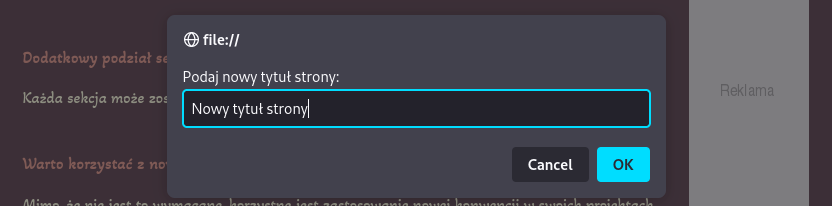
\includegraphics[width=\textwidth]{img/chapter3/js.example.prompt.png}
    \caption{Monit wyświetlony na skutek zdarzenia kliknięcia kursorem na logo przykładowej strony HTML}
    \label{fig:js.example.prompt}
\end{figure}

Po potwierdzeniu wprowadzenia nowej nazwy, podmieniona zostaje wartość pola textContent w obiekcie reprezentującym element HTML. Zmiany wprowadzone przy pomocy obiektów interfejsu DOM są widoczne w strukturze dokumentu na rys. \ref{fig:js.example.after_click}.

\begin{figure}[!htbp] 
    \centering
    
\includegraphics[width=\textwidth]{img/chapter3/js.example.after_click.png}
    \caption{Nagłówek przykładowej strony HTML po wprowadzeniu nowej zawartości tytułu w monicie na rys. \ref{fig:js.example.prompt}}
    \label{fig:js.example.after_click}
\end{figure}

%%%%%%%%%%%%%%%%%%%%%%%%%%%%%%%%%%%%%%%%%%%%%%%%%%%%%%%%%%%%%%%%%%%%%%%%%%%%%%%%
\section{Nowy standard WebAssembly}
%%%%%%%%%%%%%%%%%%%%%%%%%%%%%%%%%%%%%%%%%%%%%%%%%%%%%%%%%%%%%%%%%%%%%%%%%%%%%%%%

W dzisiejszych czasach, Internet wypełniony jest interaktywną zawartością, w której najważniejszą rolę odgrywa język programowania JavaScript (JS). To z jego pomocą, twórcy aplikacji klienckich są w stanie dynamicznie manipulować elementami HTML, czy deklaracjami CSS na oczach użytkownika np. przy pomocy identyfikatorów HTML. Ponadto, umożliwia on wysyłanie żądań HTTP oraz obsługę odbioru ich odpowiedzi, za pośrednictwem dedykowanych w tym celu, interfejsów programistycznych, tworząc istotną warstwę logiki w tych aplikacjach.

Jednakże w 2015 roku, pojawił się nowy standard nazwany WebAssembly (WASM), który w 2019 roku został włączony w poczet technologii rekomendowanych przez W3C. Miał on początkowo odpowiadać na potrzebę wykonywania kodu po stronie użytkownika, z wydajnością bliską natywnej. JS pozostaje wysokopoziomowym językiem skryptowym, z pamięcią zarządzaną automatycznie oraz kodem optymalizowanym dynamicznie w czasie kompilacji w locie. WASM przypomina raczej niskopoziomowy kod asemblera, odrzucającego m.in. wtórne optymalizacje kodu oraz czytelny dla człowieka format, na rzecz bardzo szybkiej egzekucji w silniku przeglądarki \cite{wasm.concepts}.

WASM jest językiem statycznie typowanym i definiuje jedynie cztery podstawowe typy danych - liczby całkowite w wariantach 32-bit i 64-bit oraz liczby zmiennoprzecinkowe, również w wariantach 32-bit i 64-bit. Jego działanie opiera się na czterech podstawowych pojęciach opisanych poniżej:

\begin{itemize}
    \item Moduł - kompaktowy plik binarny definiujący bezstanowy kod wykonywalny. Umożliwia to współdzielenie pliku przez kilka osobnych instancji na raz. Ze względu na format binarny można przesyłać go w postaci strumienia bajtów i przeprowadzić jego interpretacje na bieżąco.
    \item Pamięć - bufor o zmiennym rozmiarze, stanowiący tablice bajtów nadpisywanych i czytanych przez niskopoziomowy system pamięci WebAssembly. Każdy z bajtów posiada własny indeks, który może zostać potraktowany jako adres w pamięci w określonych przypadkach.
    \item Tablica - bufor o zmiennym rozmiarze, służący do przechowywania referencji, które nie powinny być przechowywane jako bajty w pamięci WASM, np. referencje do funkcji.
    \item Instancja - moduł wraz z przypisaną do niego pamięcią i tablicą oraz wszystkimi zaimportowanymi wartościami. Instancja w odróżnieniu od modułu jest więc obarczona stanem.
\end{itemize}

WebAssembly nie został wprowadzony by zastąpić język JavaScript, a raczej stać się jego współpracownikiem w realizacji określonych zadań. Dzięki interfejsom programistycznym (definiujących m.in. powyższe 4 pojęcia) wprowadzonym do standardów, możliwa jest komunikacja dwukierunkowa między obiema technologiami w przeglądarce.

Przykładowo, pozwala to na szybkie wykonanie obliczeń przy pomocy zaimportowanego modułu WASM w aplikacji klienckiej, stworzonej głównie w języku JS. Analogicznie, możliwa jest nawet manipulacja strukturami DOM strony internetowej wewnątrz modułu WASM, wykorzystując JS jako mediator. Na chwilę obecną DOM i WebAssembly nie mogą komunikować się w żaden sposób bezpośrednio, jednakże rozważa się wprowadzenie tej możliwości w kolejnych wersjach standardu.

Zaletą binarnego WASM, jest możliwość zastosowania formatu, jako cel kompilacji dla innych technologii. W ten sposób, języki takie jak C++, Rust czy C\# mogą zostać wykorzystane do tworzenia funkcjonalnych modułów dla internetowych aplikacji klienckich. Przykładowymi zastosowaniami takiego rozwiązania, są szybkie obliczenia, na potrzeby renderowania grafiki przy pomocy interfejsu WebGL, przetwarzania plików audiowizualnych, obliczeń kryptograficznych czy kompresji.

Niektóre platformy programistyczne wychodzą jednak o krok dalej, umożliwiając tworzenie w pełni funkcjonalnych aplikacji klienckich, przy pomocy języków innych niż JS. Jest to możliwe, dzięki wprowadzeniu warstwy inter-operatywności, przy pomocy pośredniej technologii WASM. Z takiego właśnie rozwiązania, korzystano podczas tworzenia projektu, opisywanego dalej w niniejszej pracy.

%%%%%%%%%%%%%%%%%%%%%%%%%%%%%%%%%%%%%%%%%%%%%%%%%%%%%%%%%%%%%%%%%%%%%%%%%%%%%%%%
\section{Najważniejsze cechy protokołu HTTP}
%%%%%%%%%%%%%%%%%%%%%%%%%%%%%%%%%%%%%%%%%%%%%%%%%%%%%%%%%%%%%%%%%%%%%%%%%%%%%%%%

W poprzednich sekcjach, omówione zostały najważniejsze technologie webowe, pozwalające użytkownikom na interakcje ze stronami internetowymi, zgodnie z wizją Tima Bernesa-Lee. Jednakże, ich prawidłowe funkcjonowanie jest możliwe, dzięki zastosowaniu protokołu HTTP \cite{http.docs}, dostarczającemu ich zasoby do klienta.

Aby przybliżyć naturę tego protokołu, w kontekście opisywanej pracy, poniżej wypunktowano kilka jego najważniejszych cech ze stosownymi objaśnieniami:

\begin{itemize}
    \item HTTP jest protokołem warstwy aplikacji - oznacza to, że stanowi część najbardziej abstrakcyjnej warstwy Internetu. W odróżnieniu od protokołów TCP (warstwa transportu) oraz IP (warstwa internetowa) jego głównym zadaniem jest reprezentacja przesyłanych danych w sposób łatwo interpretowany przez interfejsy aplikacji klienckich i serwerowych.
    \item Stanowi on przykład implementacji modelu klient-serwer, w którym, zadaniem klienta jest wysłanie zapytania do serwera i interpretacja odpowiedzi jakiej udzielił.
    \item Bezstanowość oznacza, że między odpowiedziami na kolejne żądania, serwer nie przetrzymuje informacji o ich stanie. Substytutem do tego, są tzw. ciasteczka, stanowiące mechanizm stanu sesji, związany bezpośrednio z protokołem HTTP. Więcej informacji o nich zamieszczono w następnej sekcji pracy.
\end{itemize}

Żądanie HTTP składa się z trzech wymaganych elementów, ale może zawierać dodatkowo, kilka opcjonalnych nagłówków oraz ciało (body) reprezentujące przesyłane dane. Jego treść zawsze rozpoczyna tzw. metoda.

\begin{itemize}
    \item Metoda GET odpowiada za pobieranie zasobów z serwera. W odpowiedzi można spodziewać się zwrotu treści dokumentu HTML, pliku graficznego lub nawet pojedynczego łańcucha znaków.
    \item Metoda POST służy głównie do tworzenia encji w bazie danych lub np. obsługi procesu uwierzytelniania użytkownika w systemie. W odróżnieniu od żądań GET przesyła w swoim ciele dane, które następnie przetworzy aplikacja serwerowa.
    \item Kolejnymi często stosowanymi metodami są PUT i PATCH, służące do aktualizacji danych encji w bazie danych. Podobnie jak żądania POST zwykle zawierają w swoim ciele dane, jednak odróżnia je sposób wprowadzania zmian. PUT symbolizuje ponowne wstawienie całego rekordu w bazie ze zaktualizowanymi wartościami, podczas gdy PATCH skupia się na podmianie wybranych wartości w jego komórkach.
    \item Ostatnią podstawową metodą jest DELETE, służąca do usuwaniu zasobów po stronie serwera, wykorzystując np. klucz główny rekordu w bazie danych.
\end{itemize}

Metody pełnią głównie rolę semantyczną, pozwalając programistom na łatwiejsze zrozumienie, jaką rolę powinny odgrywać tworzone akcje. Ich rolą nie jest ograniczenie możliwości wykonywanych operacji po stronie serwera.  Nie narzucają również ograniczeń na dołączone w żądaniu nagłówki i zawartość danych w ciele żądania.

\begin{lstlisting}[caption=Przykładowe rządanie HTTP, label=lst:http.example_request]
GET /?q=HTTP&t=h_ HTTP/2
Host: duckduckgo.com
User-Agent: Mozilla/5.0 (Windows NT 10.0; rv:91.0) Gecko/20100101 Firefox/91.0
Accept: text/html,application/xhtml+xml,application/xml;q=0.9,image/avif,image/webp,*/*;q=0.8
Accept-Language: en-US,en;q=0.5
Accept-Encoding: gzip, deflate, br
DNT: 1
Connection: keep-alive
Upgrade-Insecure-Requests: 1
Sec-Fetch-Dest: document
Sec-Fetch-Mode: navigate
Sec-Fetch-Site: same-origin
Sec-Fetch-User: ?1
TE: trailers
\end{lstlisting}

Pozostałymi dwoma niezbędnymi elementami żądania, jest ścieżka określająca adres punktu końcowego na który, powinno zostać wysłane żądanie oraz kod wykorzystywanej wersji protokołu. Umieszczenie kolejno metody, adresu oraz kodu wersji, oddzielonych spacjami w pierwszym wierszu przesyłanych danych, tworzy prawidłowe i kompletne żądanie HTTP. 

W celu wykorzystania pełni potencjału żądań warto jest zastosować opcjonalne nagłówki. Są one parami wartości przypisanych do zdefiniowanych przez standard kluczy, oddzielonych od siebie znakiem nowej linii. Przykładowo, wykorzystanie nagłówka "Host" pozwala nam zdefiniować prefiks do ścieżki punktu końcowego i znacznie skrócić pierwszy wiersz żądania.

Fragment żądania nazywany ciałem, od jego nagłówków odgranicza jedna pusta linia. Najczęściej dane sformatowane są jako notacja obiektowa JavaScript (JSON) przez wzgląd na jej czytelność dla ludzi i maszyn. Może on także przedstawiać dane w formacie binarnym lub dowolną treść tekstową.

Odpowiedzi HTTP od żądań, odróżnia zawartość ich pierwszej linii. Zamiast metody, pierwszym jej elementem, jest kod wersji stosowanego protokołu, drugim kod statusu wykonanego żądania, a ostatnim wiadomość opisująca ten status. W przypadku dodatkowych nagłówków oraz ciała odpowiedzi, sytuacja jest identyczna jak dla żądań.

\begin{lstlisting}[caption=Odpowiedź HTTP na przykładowe żądanie z listingu \ref{lst:http.example_request}, label=lst:http.example_response]
HTTP/2 200 OK
server: nginx
date: Sat, 29 Jan 2022 20:03:24 GMT
content-type: text/html; charset=UTF-8
vary: Accept-Encoding
...
x-duckduckgo-locale: en_US
content-encoding: br
X-Firefox-Spdy: h2

<!DOCTYPE html>...
\end{lstlisting}

Wśród kodów statusu odpowiedzi HTTP, wyróżniamy pięć głównych podgrup, obsługujących pokrewne ze sobą sytuacje. Każdy z kodów statusu jest trzycyfrową liczbą całkowitą. Pierwsza z cyfr określa przynależność do jednej z podgrup, a pozostałe dwie służą sprecyzowaniu z jakim przypadkiem klient ma do czynienia. Statusy x00 najczęściej reprezentują sytuacje, w których trudno jest skonkretyzować naturę otrzymanego wyniku.

\begin{itemize}
    \item Kody 1xx odpowiadają za sytuacje, w których klient może kontynuować wykonywaną operację lecz powinien otrzymać pewne metadane dotyczące swojego żądania. Na przykład, stosując w żądaniu nagłówek "Expected: 100-continue" można wymusić na serwerze przesłanie informacji zwrotnej ze statusem "100 Continue", świadczącej o prawidłowym użyciu nagłówków w żądaniu HTTP.
    \item Statusy powodzenia 2xx określają, że żądanie zostało wykonane pomyślnie. Przykładowo "204 Created" informuje o pomyślnym utworzeniu nowego zasobu po stronie serwera.
    \item Przekierowania 3xx obsługują wszystkie te sytuacje, w których zaszła potrzeba przekierowania żądania użytkownika na inny adres. Ciekawym przykładem jest status "304 Not Modified" implikujący możliwość skorzystania z utworzonej wcześniej w pamięci podręcznej kopii zasobu, ze względu na brak zmian w jego treści od ostatniego uzyskanego dostępu.
    \item Niepowodzenia żądań 4xx - jednoznacznie wskazują na to, że mimo uzyskania połączenia z serwerem i obsłużenia żądania, operacja zakończyła się niepowodzeniem. Jednym z najpopularniejszych kodów statusu w internecie, jest bez wątpienia "404 Not Found" informujący o tym, że punkt końcowy do którego chcemy uzyskać dostęp nie został odnaleziony. 
    \item Wewnętrzne błędy serwera 5xx stanowią zdecydowanie najbardziej zatrważające ze statusów odpowiedzi HTTP. W ich przypadku, serwer nie działa poprawnie, dlatego nie jest w stanie obsłużyć przesyłanego żądania. 
\end{itemize}

Dzięki swej prostocie, protokół HTTP jest w stanie zapewnić deweloperom bardzo przejrzysty i dobrze udokumentowany sposób komunikacji klienta z serwerem. Począwszy od sformułowania standardu, liczba jego zastosowań wciąż rośnie i prawdopodobnie pozostanie on kluczowym rozwiązaniem w dziedzinie informatyki przez kilka najbliższych dekad.

%%%%%%%%%%%%%%%%%%%%%%%%%%%%%%%%%%%%%%%%%%%%%%%%%%%%%%%%%%%%%%%%%%%%%%%%%%%%%%%%
\section{Ciasteczka HTTP, pamięć sesji i pamięć lokalna}
%%%%%%%%%%%%%%%%%%%%%%%%%%%%%%%%%%%%%%%%%%%%%%%%%%%%%%%%%%%%%%%%%%%%%%%%%%%%%%%%

W poprzedniej sekcji, przedstawione zostały podstawowe założenia protokołu HTTP, który w rękach wprawnego inżyniera oprogramowania, stanowi bardzo uniwersalne narzędzie. Jednakże, jego bezstanowość zainicjowała potrzebę wykorzystania dodatkowego mechanizmu, odpowiedzialnego za przechowywanie informacji o stanie klienta bądź serwera.

Na potrzebę tą, jako pierwsze odpowiedzieć miały ciasteczka HTTP, nazywane w skrócie "ciasteczkami", opisane w dokumencie RFC 6265 \cite{cookies.rfc6265}. Stan sesji klienta, bądź serwera, jest przechowywany przy ich pomocy w przeglądarce użytkownika, jako pliki składujące klucz oraz przypisaną do niego wartość \cite{cookies.docs}.

\begin{lstlisting}[caption=Przykładowa odpowiedź HTTP wykorzystująca nagłówek Set-Cookie, label=lst:cookies.setCookies]
HTTP/2 200 OK
Content-Type: text/html
Set-Cookie: ciasteczko_1=wartość_1
Set-Cookie: ciasteczko_2=wartość_2
...

[Zawartość strony]
\end{lstlisting}

Do tworzenia plików ciasteczek służy nagłówek Set-Cookie, dołączany w odpowiedzi HTTP przez serwer. Na listingu \ref{lst:cookies.setCookies} zaprezentowano bardzo prosty przykład jego wykorzystania tworzący dwa pliki ciasteczek, nieobarczonych żadnymi dodatkowymi ograniczeniami, nazwane kolejno ciasteczko\_1 oraz ciasteczko\_2.

\begin{lstlisting}[caption=Przykładowe żądanie HTTP wykorzystujące nagłówek Cookies, label=lst:cookies.cookies_header]
GET /search HTTP/2
Cookies: ciasteczko_1=wartość_1; ciasteczko_2=wartość_2
\end{lstlisting}

W wyniku składowania plików ciasteczek w pamięci przeglądarki, zostają one automatycznie dołączone do każdego kolejnego żądania wysyłanego na serwer, który je utworzył. Przeglądarka robi to przy pomocy nagłówka Cookies w sposób przedstawiony na listingu \ref{lst:cookies.cookies_header}.

Mechanizm plików ciasteczek posiada kilka dodatkowych funkcjonalności, umożliwiających wykorzystanie ich w bardziej wyspecjalizowany sposób. Przy pomocy tzw. atrybutów ciasteczka jesteśmy w stanie wyznaczyć okres ich ważności, zabezpieczyć ich zawartość przed niewłaściwym użyciem, a także uściślić sposób ich automatycznego załączania.

\begin{lstlisting}[caption=Przykładowe użycie atrybutu terminu ważności ciasteczka HTTP, label=lst:cookies.expires]
Set-Cookie: ciasteczko_1=wartość_1; Expires=Tue, 08 Feb 2022 10:00:00 GMT;
Set-Cookie: ciasteczko_2=wartość_2; Max-Age: 20;
\end{lstlisting}

Ciasteczko, dla którego nie ustawiono terminu ważności, jest ważne do końca trwania obecnej sesji przeglądarki. W przypadku skorzystania z atrybutu Expires, serwer jest w stanie ustalić moment, w którym plik utraci swą ważność. Nowszy atrybut Max-Age ułatwia pracę z tym mechanizmem, pozwalając na określenie, po ilu sekundach od momentu przesłania ciasteczka przez serwer, ulega ono przedawnieniu. Po upływie tego terminu, ciasteczko domyślnie zostaje usunięte z pamięci przeglądarki.

\begin{lstlisting}[caption=Przykładowe użycie atrybutów dostępu ciasteczka HTTP, label=lst:cookies.secure]
Set-Cookie: ciasteczko_1=wartość_1; Secure; HttpOnly
Set-Cookie: ciasteczko_2=wartość_2; HttpOnly
\end{lstlisting}

Kolejnymi atrybutami ciasteczek są flagi Secure oraz HttpOnly, użyte przykładowo na listingu \ref{lst:cookies.secure}, odpowiadające za zakres dostępu. W przypadku pierwszego z nich, blokuje się dostęp do wartości ciasteczek, żądaniom stosującym niezaszyfrowany wariant protokołu HTTP. Drugi, odpowiada za zablokowanie dostępu do ciasteczek językowi JavaScript, za pośrednictwem interfejsu DOM.

\begin{lstlisting}[caption=Przykładowe użycie atrybutów punktu docelowego ciasteczka HTTP, label=lst:cookies.domain]
Set-Cookie: ciasteczko_1=wartość_1; Domain=duckduckgo.com; Path=/search
Set-Cookie: ciasteczko_2=wartość_2; SameSite=Strict
\end{lstlisting}

Na listingu \ref{lst:cookies.domain} przedstawiono użycie trzech atrybutów, mających na celu uściślenie, do których żądań, należy dołączyć dane ciasteczko. W przypadku nie zastosowania atrybutu Domain, ciasteczka będą dołączane tylko do żądań prowadzących ściśle do hosta, który je utworzył. Atrybutu można użyć w celu całkowitej zmiany domeny lub adresu, jednakże powoduje on również rozszerzenie zakresu docelowych żądań na wszystkie poddomeny określonego adresu.

Atrybut Path, zawęża pulę żądań docelowych, do przypadków dotyczących konkretnych ścieżek. Przykładowo ciasteczko\_1 z listingu \ref{lst:cookies.domain} zostałoby dołączone jedynie do tych żądań, dla których domeną serwera byłoby "duckduckgo.com" lub jedna z jej poddomen np. "html.duckduckgo.com". Dodatkowo, lista ta podlega drugiemu przefiltrowaniu ścieżek do przypadków, w których zaczyna się ona od "/search", np. "/search", "/search/images" czy "/search/maps/pl".

Dodatkowy atrybut SameSite o podobnym zastosowaniu, odpowiada za przyjętą zasadę tolerancji wobec obcych domen. Od najnowszych zmian w standardzie ciasteczek, porównuje on wersje niezaszyfrowaną (http) oraz zaszyfrowaną (https) danej domeny, jako dwa osobne adresy. Jako atrybut typu wyliczeniowego, posiada trzy możliwe wartości:

\begin{itemize}
    \item Strict - wartość z pliku ciasteczka zostanie dołączona jedynie do żądań wychodzących ze strony, która początkowo je utworzyła.
    \item Lex - dodatkowo rozbudowuje powyższy tryb o przypadki przechodzenia z innej domeny na stronę, która utworzyła ciasteczko. Jest on trybem domyślnym.
    \item None - ciasteczka są wysyłane w żądaniach pochodzących zarówno ze strony stanowiącej ich źródło, jak i podczas przechodzenia na nią z obcej domeny, jednakże implikuje przymus użycia atrybutu Secure.
\end{itemize}


Pliki ciasteczek, dzięki swym atrybutom, umożliwiają automatyzację niektórych procesów związanych z przesyłaniem ich zawartości między klientem a serwerem. Przy odpowiednim zastosowaniu atrybutów, pozwalają magazynować stan sesji użytkownika przez ściśle określony czas i zadbać o jego bezpieczeństwo przed wieloma rodzajami ataków. 

Niestety, ciasteczka w dobie współczesnego internetu posiadają również wady. Pozwalają na przechowywanie maksymalnie 4096 bajtów danych, w ramach pojedynczego pliku. Zwykle, jest to pojemność wystarczająca do przechowywania metadanych użytkownika lub jego tokenu uwierzytelniającego (zalecany sposób przechowywania tych tokenów). Jednakże, twórcy przeglądarek internetowych postanowili odpowiedzieć na potrzebę większej rozszerzalności rozwiązań webowych.

\begin{figure}[!htbp] 
    \centering
    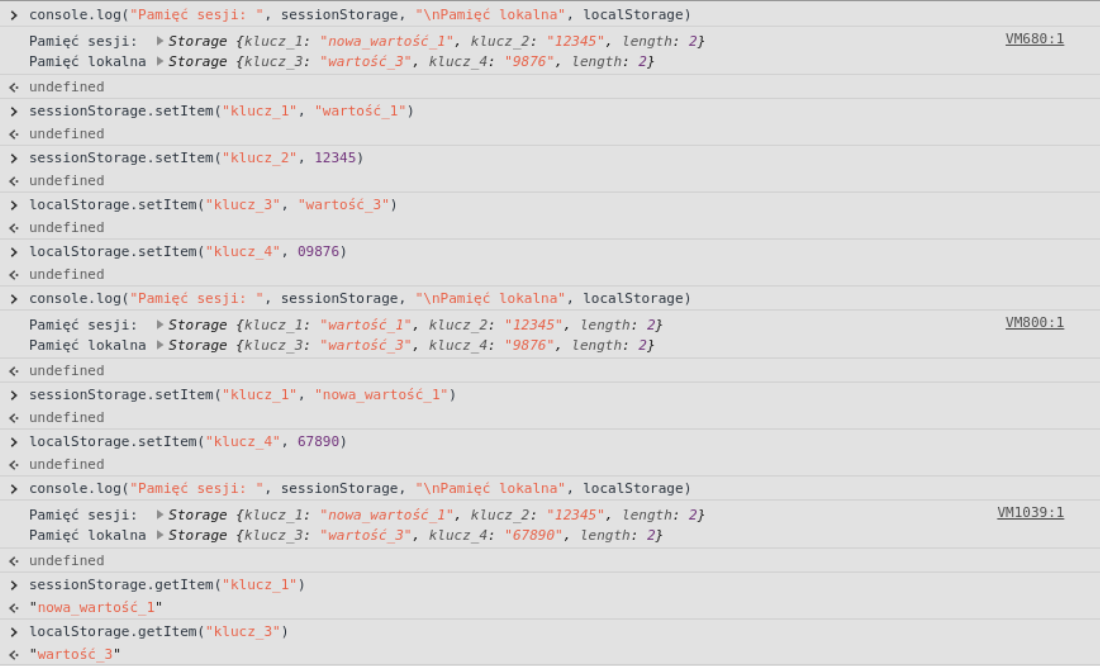
\includegraphics[width=\textwidth]{img/chapter3/storage.setting_values.png}
    \caption{Tworzenie, modyfikacja oraz dostęp do par klucz-wartość w pamięci sesji i pamięci lokalnej}
    \label{fig:storage.setting_values}
\end{figure}

Z tego powodu, zrodziła się idea interfejsu programistycznego pamięci webowej (Web Storage API), podzielonej na przestrzeń pamięci sesji oraz pamięci lokalnej \cite{web_storage.docs}. Opiera się ona na założeniu przypisywania danych do klucza. Jednakże, w odróżnieniu od plików ciasteczek, umożliwiła ona przechowywanie plików o pojemności od 5 do 10 megabajtów danych (w zależności od implementacji). Ponadto, dostęp do tej pamięci odbywa się w pełni za pośrednictwem skryptów JavaScript po stronie klienta. Na rys. \ref{fig:storage.setting_values} ukazano proces tworzenia, modyfikacji oraz dostępu do par klucz-wartość w obu rodzajach pamięci webowej przy pomocy jej interfejsu. Zarówno pamięć sesji, jak i pamięć lokalna, przypisane są do konkretnego źródła (domeny) w obrębie którego, można z nich skorzystać.

\begin{figure}[!htbp] 
    \centering
    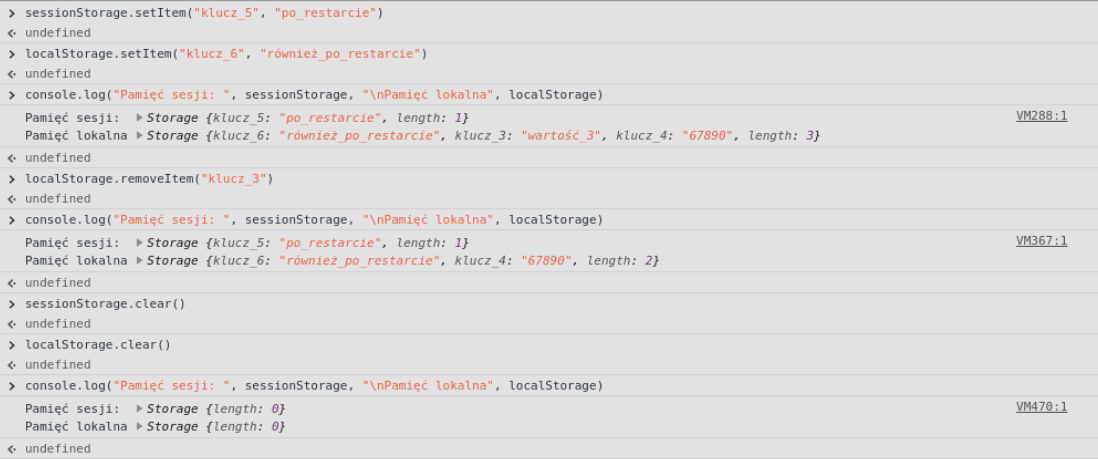
\includegraphics[width=\textwidth]{img/chapter3/storage.removing_values.png}
    \caption{Stan par klucz-wartość w pamięci sesji i pamięci lokalnej po ponownym uruchomieniu instancji przeglądarki oraz ręczne metody ich usuwania}
    \label{fig:storage.removing_values}
\end{figure}

Pamięć sesji, zgodnie ze swoją nazwą, służy do przechowywania danych, które zostaną automatycznie wykasowane z pamięci przeglądarki po zamknięciu instancji, w której zostały utworzone. Dane w pamięci lokalnej są w niej przetrzymywane, nawet po zamknięciu i ponownym uruchomieniu przeglądarki. Jedynym sposobem na usunięcie z niej zapisanych par kluczy i wartości, jest ręczne zastosowanie interfejsu programistycznego w skryptach strony lub wyczyszczenie ich z pamięci podręcznej, z poziomu ustawień samego programu. Procesy te zostały ukazane na rys. \ref{fig:storage.removing_values}, uchwyconym po ponownym uruchomieniu przeglądarki internetowej z rys. \ref{fig:storage.setting_values}.

Pliki ciasteczek i pamięć webowa, nie powinny być traktowane jako rywalizujące ze sobą rozwiązania tego samego problemu. Dzięki funkcjonalnościom, możliwym do zastosowania przy pomocy atrybutów ciasteczek oraz automatyzacji ich załączania, są one szczególnie pomocne w składowaniu danych stanu sesji istotnych dla aplikacji serwerowych systemu. Świetnie sprawdzą się w scenariuszach, w których liczy się bezpieczeństwo danych, łatwe przekazywanie metainformacji do wykorzystania przez inne domeny (np. logowanie B2C) oraz termin ważności tych informacji. 

Pamięć webowa, dzięki swej prostocie i ścisłemu związkowi ze skryptami wykonywanymi po stronie klienta, idealnie nadaje się do przechowywania danych, intensywnie wykorzystywanych przez aplikacje klienckie. To właśnie w nich, wykorzystany może zostać potencjał bardziej obszernych plików konfiguracyjnych, które może przechować dla nich nowszy mechanizm składowania stanu.

%%%%%%%%%%%%%%%%%%%%%%%%%%%%%%%%%%%%%%%%%%%%%%%%%%%%%%%%%%%%%%%%%%%%%%%%%%%%%%%%
\section{Tokeny JWT jako mechanizm autoryzacji}
%%%%%%%%%%%%%%%%%%%%%%%%%%%%%%%%%%%%%%%%%%%%%%%%%%%%%%%%%%%%%%%%%%%%%%%%%%%%%%%%

Jedną z ważniejszych oraz mniej oczywistych pozycji w stanie sesji klienta, stanowią dane autoryzacyjne klienta. W ostatnich latach, najpopularniejszym rozwiązaniem tego zagadnienia stały się tokeny JSON Web Tokens (JWT) \cite{jwt.rfc7519}. Swą popularność nad starszymi rozwiązaniami wykorzystującymi format XML \cite{jwt.auth0}, zawdzięczają kilku zaletom:

\begin{itemize}
    \item JWT oferują większe bezpieczeństwo, dzięki łatwości podpisywania tokenów w formacie JSON. Umożliwiają skorzystanie z puli algorytmów HMAC (bazującego na kluczu-sekrecie), RSA i ECDSA (klucz prywatny i publiczny). W porównaniu do podpisywania danych w formacie XML jest to o wiele prostszy proces.
    \item Obiektowość formatu JSON, jest powodem, nie tylko jego wysokiej czytelności dla ludzi, ale również, łatwego parsowania danych do obiektów w aplikacjach klienckich i serwerowych.
    \item Tokeny są bardzo kompaktowe, w porównaniu do  rozwiązań bazujących na formacie XML. Dają możliwość przesłania większej ilości danych w mniejszej ilości bajtów, w zakodowanej formie JWT.
\end{itemize}

Token JWT składa się z trzech części: nagłówka, ładunku i podpisu. Wszystkie trzy części przedstawiono w formie zakodowanej i zdekodowanej na rys. \ref{fig:jwt.parts}. Dwie pierwsze części, stanowią obiekty JS (znane z formatu JSON), ostatnia część jest wynikową operacji algorytmu podpisującego token.

\begin{figure}[!htbp] 
    \centering
    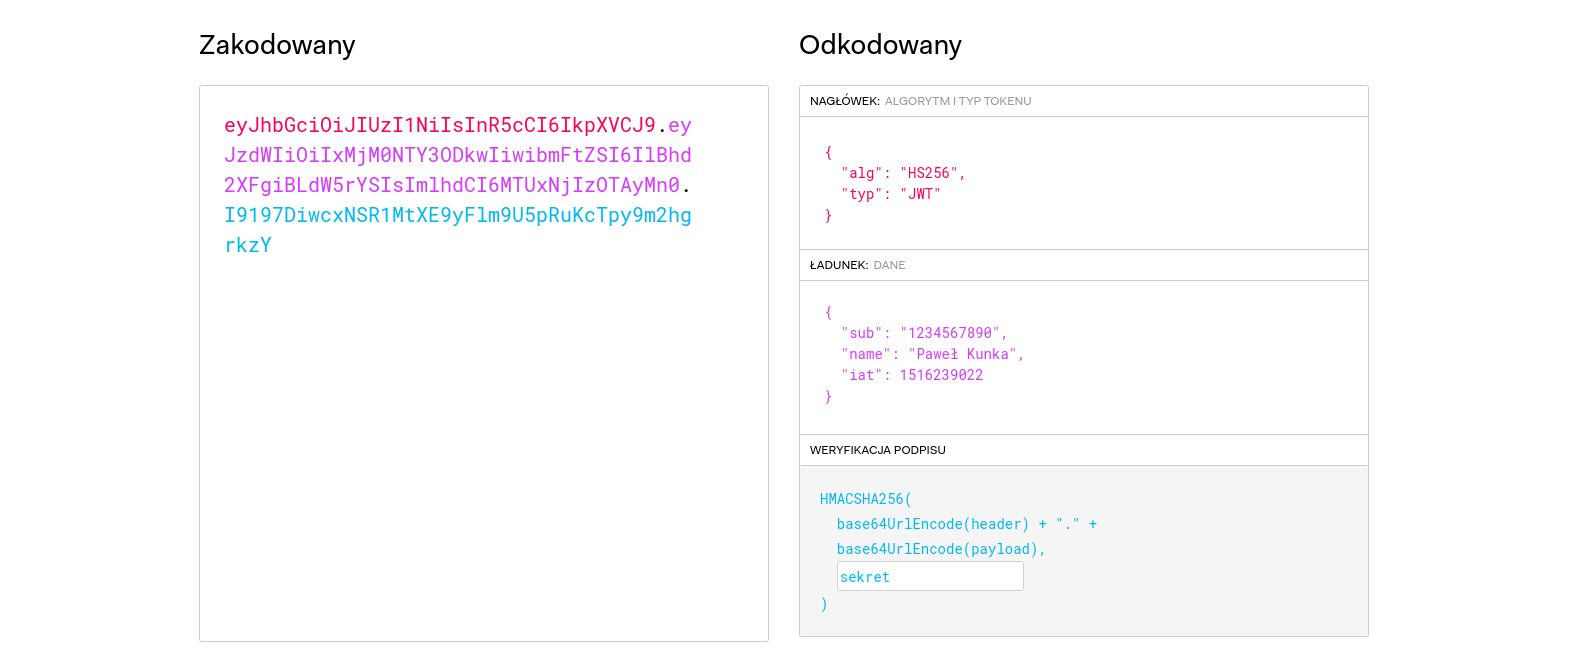
\includegraphics[width=\textwidth]{img/chapter3/jwt.parts.png}
    \caption{Analiza części składowych przykładowego tokenu JWT w formie zakodowanej i odkodowanej}
    \label{fig:jwt.parts}
\end{figure}

\begin{itemize}
    \item Nagłówek tokenu, przetrzymuje informacje o algorytmie używanym przy podpisywaniu i szyfrowaniu tokenu (pole alg) oraz typie tokenu (pole typ).
    \item Ładunek tokenu może, lecz nie musi, zawierać kilka pól tzw. twierdzeń, udostępniających dodatkowe informacje o encji, której poświęcony jest token np. dane użytkownika. Specyfikacja tokenów JWT, wyróżnia kilka twierdzeń zastrzeżonych, które służą konkretnym zastosowaniom. Ma to na celu zwiększenie kompatybilności rozwiązań. Przykładowo, użyte pola sub i iat służą kolejno do określenia identyfikatora encji, której został poświęcony token oraz czasu jego wyemitowania. Pole name jest twierdzeniem zdefiniowanym dodatkowo przez twórcę tokenu.
    \item Podpis jest ciągiem znaków, otrzymanym w wyniku zastosowania funkcji algorytmu podpisującego, określonego w nagłówku. Funkcja ta, przyjmuje za argumenty treść nagłówka i ładunku, oddzielonego kropką oraz tzw. sekret. Sekret jest ciągiem znaków, trzymanym w bezpiecznym miejscu, służącym do podpisywania i szyfrowania danych, po stronie jego właściciela. Podpis, pozwala potwierdzić autentyczność przesłanych informacji oraz czy wartości przedstawionych twierdzeń nie zostały zmodyfikowane.
\end{itemize}

Ze względu na bardzo mały rozmiar tokenów JWT, do ich przechowywania można zastosować zarówno pliki ciasteczek, jak i pamięć webową. Przez wzgląd na cechy ciasteczek, wymienione w poprzedniej sekcji, często stosuje się je w przypadku tokenów służących autoryzacji.

\begin{lstlisting}[caption=Użycie tokenu JWT jako mechanizm autoryzacji w żądaniu HTTP, label=lst:jwt.authorization]
Authorization: Bearer nagłówek_jwt.ładunek_jwt.podpis_jwt
\end{lstlisting}

Aby zastosować JWT w optymalny sposób, należy dołączyć do żądań, przesyłanych na zabezpieczone ścieżki serwera, nagłówek Authorization. Przykładowe użycie, zamieszczono na listingu \ref{lst:jwt.authorization}. Jego zawartość określa schemat wykorzystujący JWT jako element pośredni przenoszący dane (Bearer). 

%%%%%%%%%%%%%%%%%%%%%%%%%%%%%%%%%%%%%%%%%%%%%%%%%%%%%%%%%%%%%%%%%%%%%%%%%%%%%%%%
\section{Aplikacje serwerowe REST}
%%%%%%%%%%%%%%%%%%%%%%%%%%%%%%%%%%%%%%%%%%%%%%%%%%%%%%%%%%%%%%%%%%%%%%%%%%%%%%%%

W przypadku aplikacji serwerowych, zdecydowanie największą popularnością, cieszy się styl architektoniczny Reprezentacyjnego Transferu Stanu (REST lub aplikacja RESTowa). Jej koncepcję, zaproponował po raz pierwszy, doktor Roy Thomas Fielding w swojej pracy naukowej z roku 2000 \cite{restapi.genesis}. 

\begin{figure}[!htbp] 
    \centering
    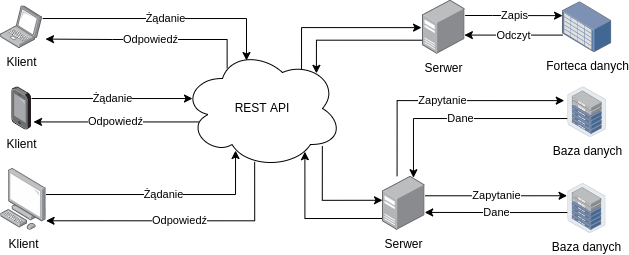
\includegraphics[width=\textwidth]{img/chapter3/rest.overview.png}
    \caption{Rola interfejsów programistycznych REST w systemach internetowych}
    \label{fig:rest.overview}
\end{figure}

Posiada on, kilka podstawowych założeń, nakładających na tworzone aplikacje ograniczenia, które ostatecznie przyczyniają się do tworzenia bardziej spójnego i rozszerzalnego rozwiązania. Poniżej przedstawiono podstawy architektury REST:

\begin{itemize}
    \item Ujednolicenie interfejsów - zasada mające swoje podłoże w paradygmacie ogólności inżynierii oprogramowania. Każdy interfejs, wskazujący na ten sam zasób, powinien wyglądać identycznie dla wszystkich źródeł swego pochodzenia np. dla każdego klienta. Interfejs REST powinien przekazywać ujednoliconą formę reprezentacji zasobu, na której powinien pracować klient. Interfejsy zasobów, powinny być jak najbardziej kompaktowe, jednocześnie zawierając w sobie wystarczającą porcję informacji opisujących przesyłaną wiadomość.
    \item Model klient-serwer - aplikacja kliencka powinna być świadoma istnienia jedynie tych identyfikatorów (ścieżek URI), które prowadzą do zasobów dostarczanych przez aplikacje serwerową. Jedyną ścieżką komunikacji między obydwoma programami powinien zostać protokół HTTP lub inny, jasno określony w dokumentacji interfejsu.
    \item Bezstanowość żądań - podobnie jak w przypadku protokołu HTTP, żądania REST są bezstanowe, wszystkie powinny w sobie zawierać wystarczającą ilość informacji, potrzebnych do ich przetworzenia i uzyskania odpowiedzi. Aplikacja serwerowa nie przetrzymuje informacji o statusie wcześniejszych żądań i uniemożliwia komunikację między nimi w ten sposób. Odpowiedzialność za przetrzymywanie stanu sesji może jednak zostać przerzucona na aplikację kliencką.
    \item Buforowalność - cecha zapewniająca w dłuższej perspektywie, skalowalność aplikacji serwerowej oraz lepszą wydajność aplikacji klienckiej. Aplikacja REST powinna udostępniać informacje o możliwości buforowania (przetrzymywania w pamięci podręcznej) otrzymanych wcześniej odpowiedzi po stronie klienta (lub serwera). Przykładowo, powinno być możliwe buforowanie obrazków, których znacznik czasu zapisu nie uległ zmianie w żądaniach poprzednich.
    \item Warstwowość - czasami to, co opisujemy jako aplikację RESTową, stanowi w rzeczywistości wiele pomniejszych, współpracujących ze sobą programów (np. mikro-serwisów). Cecha warstwowości opisuje abstrakcyjne założenie, zgodnie z którym, aplikacje klienckie, ani serwerowe nie zostają poinformowane, czy faktycznie komunikują się z końcowym wykonawcą danej operacji. Nie mają prawa żądać tej informacji, przyjmując interfejs programistyczny REST API jako obraz aplikacji serwerowej.
    \item Kod na żądanie - opcjonalna cecha REST, zakładająca dostarczenie części funkcjonalności systemu internetowego, w postaci kodu wykonywalnego po stronie użytkownika. Zgodnie z tą zasadą, taki kod powinien zostać uruchomiony jedynie za zgodą aplikacji klienckiej.
\end{itemize}

Opisane powyżej podstawowe założenia interfejsów programistycznych REST opierają się na pojęciu zasobów. Zasób jest pojęciem abstrakcyjnym, mogącym opisywać dowolną informację np. dokument HTML, obrazek, obiekt JS lub kolekcję takich obiektów.

Każdy zasób, posiada swój unikalny identyfikator, wykorzystywany w komunikacji między komponentami klienta i serwera. Stan zasobu nazywa się jego reprezentacją i dzieli na trzy główne składowe: dane zasobu, metadane zasobu, opisujące jego dane oraz łącza, które mogą okazać się pomocne przy zmianie jego stanu. Format danych reprezentacji, określa się jako typ medialny, który wykorzystuje się do określenia sposobu przetwarzania danego zasobu \cite{restapi.media_types.rfc6838}.

Przykładowo, dzięki typom medialnym zasobów, dokumenty HTML, arkusze CSS oraz obrazy, mogą zostać wyświetlone przez przeglądarkę, a dane przesłane w formacie JSON zmapowane na obiekty w aplikacji klienckiej lub serwerowej. Reprezentacja zasobów jest sama dla siebie opisem i nie zrzuca odpowiedzialności zinterpretowania swojej zawartości na klienta, ani serwer.

Istotnym elementem aplikacji RESTowych są również metody zasobów. Wykorzystuje się je w celu określenia, jaką operację należy zastosować na stanie zasobu. Bardzo często, metody zasobów traktuje się w sposób tożsamy z różnymi metodami żądań HTTP np. GET dla metody odczytującej zasób, POST dla metody tworzącej, PUT jako metoda aktualizacji, a DELETE jako usunięcie zasobu. Dzięki metodom zasobów można przeprowadzić kilka różnych operacji na tym samym zasobie, wykorzystując pojedynczy identyfikator (URI).

\begin{figure}[!htbp] 
    \centering
    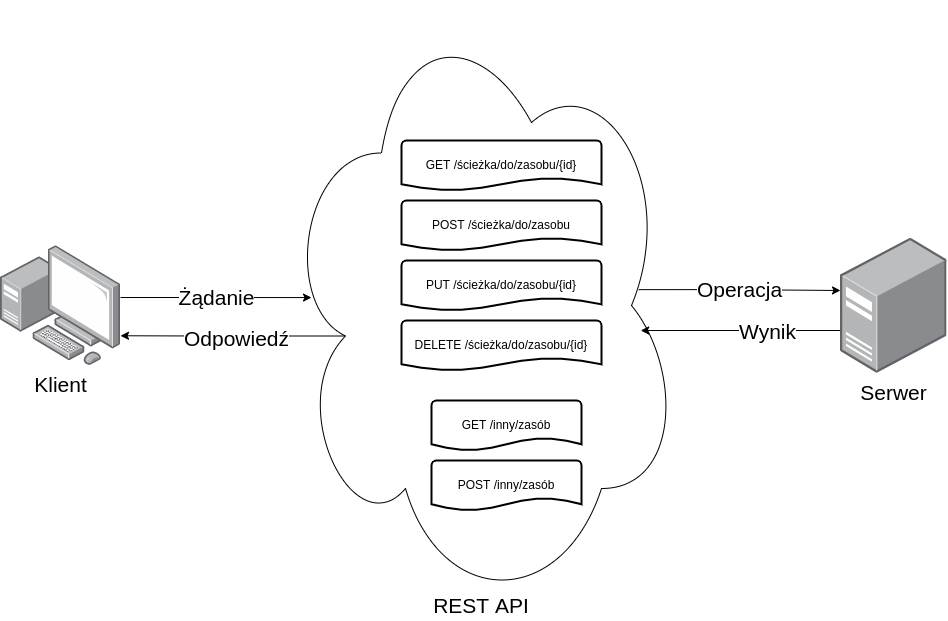
\includegraphics[width=\textwidth]{img/chapter3/rest.endpoints.png}
    \caption{Dostęp do zasobów poprzez punkty końcowe interfejsu REST}
    \label{fig:rest.endpoints}
\end{figure}

Podsumowując, interfejsy REST zakładają dostęp do funkcjonalności (operacji) i danych reprezentowanych przez jednostki zwane zasobami. Dostęp do danego zasobu odbywa się za pośrednictwem jego  ujednoliconego identyfikatora (URI) oraz odpowiedniej metody REST określającej rodzaj operacji do przeprowadzenia na zasobie.

Zasoby są wymieniane między klientem, a serwerem, w postaci swoich reprezentacji, które mogą definiować różne typy medialne np. tekst, HTML, XML, JSON czy PNG. Dzięki metadanym, możliwe jest buforowanie wybranych zasobów w celu zwiększenia wydajności systemu.

Reprezentacje zasobów przesyłane są między klientem a serwerem przy pomocy standaryzowanych interfejsów protokołu. W przypadku REST najczęściej jest to protokół HTTP, lecz architektura nie wymusza jego zastosowania. Ważne jest natomiast to, by serwer nie przetrzymywał stanu obsłużonych żądań ani sesji poszczególnych klientów.

%%%%%%%%%%%%%%%%%%%%%%%%%%%%%%%%%%%%%%%%%%%%%%%%%%%%%%%%%%%%%%%%%%%%%%%%%%%%%%%%
\section{Mechanizmy mapowania obiektowo-relacyjnego}
%%%%%%%%%%%%%%%%%%%%%%%%%%%%%%%%%%%%%%%%%%%%%%%%%%%%%%%%%%%%%%%%%%%%%%%%%%%%%%%%

Jednym z najważniejszych zadań aplikacji serwerowych jest często odczyt i zapis rekordów w bazach danych. Podstawową metodą dostępu do nich są, zdefiniowane przez dostawców silników bazodanowych, języki zapytań. Istnieje jednak alternatywny sposób pracy z nimi, zakładający wprowadzenie warstwy abstrakcji między bazą danych a aplikacją serwerową. 

Mapowanie obiektowo-relacyjne (ORM) to metoda, wywodząca się z domeny programowania obiektowego, zakładająca interakcję z bazami danych przy pomocy obiektów. Kluczową rolę pełni w niej klasa kontekstu bazy danych, stanowiąca interfejs programistyczny, pomiędzy kodem aplikacji serwerowej a bazą danych. Kontekst odpowiada za tworzenie zapytań, wykonujących operacje na rzeczywistych danych, interpretując zmiany wykonane na obiektach reprezentujących kolejno: tabele, rekordy i wartości poszczególnych komórek.

\begin{figure}[!htbp] 
    \centering
    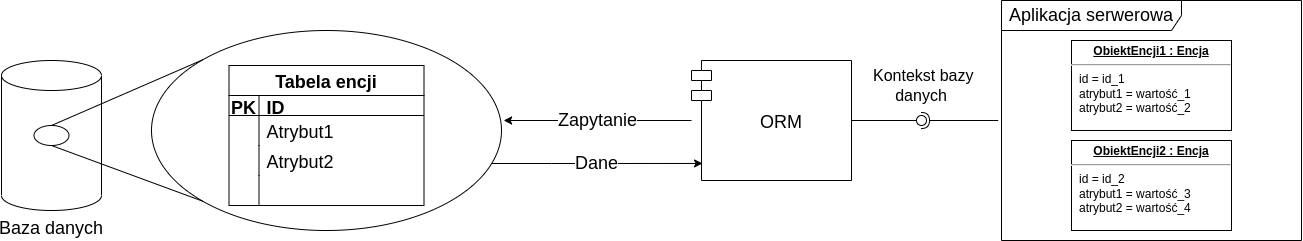
\includegraphics[width=\textwidth]{img/chapter3/orm.context.png}
    \caption{Zarys działania mapowania obiektowo-relacyjnego w aplikacjach serwerowych}
    \label{fig:orm.context}
\end{figure}

ORM najczęściej jest dołączany do projektu aplikacji jako osobna biblioteka programistyczna, zaimplementowana w języku programowania, kompatybilnym z rozwiązaniem. W praktyce, wyróżnia się trzy główne podejścia do rozpoczęcia pracy z tymi narzędziami:

\begin{itemize}
    \item Pierwszeństwo modelu bazy - metoda zakładająca wykorzystanie dedykowanego narzędzia do projektowania relacji w bazach danych, najczęściej przy pomocy diagramów opisanych w formacie pochodnym od standardu języka znaczników XML. Powstały w ten sposób model bazy danych, często może zostać wykorzystany przez ORM, do utworzenia relacji encji w bazie danych oraz wygenerowania klas encji w projekcie aplikacji serwerowej.
    \item Pierwszeństwo bazy danych - w przypadku utworzenia w pierwszej kolejności bazy danych wykorzystywanej w projekcie, ORM jest w stanie pobrać informacje o wchodzących w jej skład relacjach. Informacje służą następnie do generacji klas w kodzie projektu.
    \item Pierwszeństwo kodu - szczególnie atrakcyjna dla programistów metoda, w której najpierw tworzy się klasy encji oraz określa relacje między nimi w ramach kodu aplikacji serwerowej. Na jego podstawie, ORM jest w stanie wysyłać zapytania do silnika baz danych w celu utworzenia, modyfikacji oraz usuwania bazy aplikacji w razie potrzeby.  Zasadę funkcjonowania tej metody opisano w dalszej części sekcji, ze względu na wykorzystanie jej w projekcie systemu tworzonego w ramach niniejszej pracy.
\end{itemize}

Najważniejsze z dodatkowych pojęć w metodzie pierwszeństwa kodu stanowi migracja. Migracje stanowią dla ORM swoisty system kontroli wersji schematu bazy danych. Każda z nich jest kompleksowym opisem zbioru kwerend do wykonania, w celu zastosowania schematu bazy danych, przedstawionego w kodzie aplikacji, w ściśle określonym momencie.

W projekcie aplikacji serwerowej, migracja występuje najczęściej w postaci generowanej przez ORM klasy, zawierającej dwie metody, odpowiadające kolejno za wprowadzanie oraz wycofywanie, poczynionych w schemacie bazy zmian. Metody opisują jedynie te kwerendy, które dotyczą zmian wprowadzonych od poprzednio zdefiniowanej migracji. Za tworzenie plików migracji, a także wprowadzanie i cofanie zmian, odpowiada najczęściej, dedykowane w tym celu narzędzie konsolowe.

Zastosowanie ORM w ten sposób, pozwala na sporą oszczędność czasu na etapie tworzenia aplikacji serwerowych oraz zabezpieczenie programu przed typowymi dla języków zapytań SQL podatnościami na ataki. W związku z tym, programista może skupić się na tworzeniu lepszego rozwiązania w znajomym mu środowisku, zamiast poświęcać czas na samodzielne tworzenie zapytań. 

Narzędzia ORM oprócz wielu zalet, mają również kilka wad, na które powinien zwrócić uwagę programista. Pierwszą z nich, jest konieczność poznania sposobów generowania zapytań, w celu zastosowania przydatnych optymalizacji oraz unikania wykonywania operacji zbędnych. Kolejną wadę, stanowi nieoczywisty sposób rozwiązywania aktualizacji schematu bazy, grożący utratą danych. Podsumowując, aby w pełni korzystać z  możliwości eksploatowania narzędzi ORM, należy posiadać profesjonalną wiedzę  w tej dziedzinie.

\chapter{Projekt systemu}
%%%%%%%%%%%%%%%%%%%%%%%%%%%%%%%%%%%%%%%%%%%%%%%%%%%%%%%%%%%%%%%%%%%%%%%%%%%%%%%%
\section{Wymagania funkcjonalne}
%%%%%%%%%%%%%%%%%%%%%%%%%%%%%%%%%%%%%%%%%%%%%%%%%%%%%%%%%%%%%%%%%%%%%%%%%%%%%%%%

Projektowanie systemu informatycznego, zgodnie z założeniami inżynierii oprogramowania, rozpoczyna się od ustalenia wymagań funkcjonalnych, które powinno spełniać tworzone oprogramowanie. Wymagania te formułują zakres czynności, do których, zdolni są użytkownicy, podczas eksploatacji systemu:

\begin{itemize}
    \item Użytkownik nieuwierzytelniony posiada możliwość utworzenia konta w systemie.
    \item Użytkownik nieuwierzytelniony posiada możliwość uwierzytelnienia się, za pomocą wcześniej utworzonego konta. Jest to czynność mająca na celu, uzyskanie autoryzacji do skorzystania z reszty funkcjonalności systemu.
    \item Użytkownik uwierzytelniony może w prosty sposób, przeglądać jedną z tabel przypisanych do niego zasobów. Wyróżniamy tabele członków drużyny, sprzętu spalinowego oraz odbytych akcji.
    \item Użytkownik uwierzytelniony jest w stanie utworzyć jedną encję zasobu w przeglądanej tabeli przy pomocy formularza edycji.
    \item Użytkownik uwierzytelniony jest w stanie edytować jedną encję zasobu w przeglądanej tabeli przy pomocy formularza edycji.
    \item Użytkownik uwierzytelniony jest w stanie zaznaczyć jedną lub wiele encji zasobów w przeglądanej tabeli.
    \item Użytkownik uwierzytelniony jest w stanie permanentnie usunąć jedną lub wiele zaznaczonych encji zasobów w przeglądanej tabeli.
    \item Użytkownik uwierzytelniony ma możliwość stworzenia encji zasobu odbytej akcji, bazując na zaznaczonych członkach zespołu i sprzętu pożarowego. Formularz tworzonej akcji zawiera wtedy dodatkowe pola, pozwalające na uzupełnienie roli poszczególnych członków brygady oraz poziomu zużytego paliwa dla wybranego sprzętu.
    \item Użytkownik uwierzytelniony ma możliwość natychmiastowego usunięcia danych uwierzytelniających, z pamięci przeglądarki internetowej.
\end{itemize}

%%%%%%%%%%%%%%%%%%%%%%%%%%%%%%%%%%%%%%%%%%%%%%%%%%%%%%%%%%%%%%%%%%%%%%%%%%%%%%%%
\section{Wymagania jakościowe}
%%%%%%%%%%%%%%%%%%%%%%%%%%%%%%%%%%%%%%%%%%%%%%%%%%%%%%%%%%%%%%%%%%%%%%%%%%%%%%%%

Celem, postawionych systemowi wymagań jakościowych, jest uczynienie go łatwiejszym w obsłudze dla jego użytkowników. Spełnienie tych wymagań, ma na celu zwiększenie zadowolenia użytkownika z funkcjonalności, jakie oferuje system. Jako dodatkowy efekt, można uznać łatwiejszy rozwój systemu w procesie produkcyjnym: 

\begin{itemize}
    \item Aplikacja kliencka systemu powinna funkcjonować poprawnie z wykorzystaniem nowoczesnych przeglądarek internetowych takich jak Microsoft Edge, Google Chrome, Mozilla Firefox i Safari.
    \item Aplikacja kliencka powinna reagować na zmianę rozdzielczości ekranu urządzenia i wyświetlać się poprawnie, niezależnie od jego proporcji.
    \item Aplikacja kliencka będzie informowała o awariach i błędach w systemie w sposób jasny i zrozumiały dla użytkownika.
    \item Aplikacja kliencka ma wymagać potwierdzenia krytycznych i nieodwracalnych akcji.
    \item Wymagana jest walidacja danych w formularzach, zarówno po stronie aplikacji klienckiej jak i serwerowej.
    \item System będzie rozwijany w języku angielskim, zgodnie ze standardem rynku oprogramowania.
\end{itemize}

%%%%%%%%%%%%%%%%%%%%%%%%%%%%%%%%%%%%%%%%%%%%%%%%%%%%%%%%%%%%%%%%%%%%%%%%%%%%%%%%
\section{Diagram przypadków użycia}
%%%%%%%%%%%%%%%%%%%%%%%%%%%%%%%%%%%%%%%%%%%%%%%%%%%%%%%%%%%%%%%%%%%%%%%%%%%%%%%%

Kolejnym etapem po ustaleniu wymagań, które powinien spełnić system, powinno być sporządzenie diagramu UML przypadków użycia. Diagram ten ma na celu, przedstawienie rodzajów użytkowników oraz ich możliwości nawiązania interakcji z systemem.

Najważniejszymi elementami diagramu są jego aktorzy. Aktor najczęściej jest reprezentacją typu użytkownika systemu, jednakże w nowszych specyfikacjach UML 2.0 wyodrębnione zostały również oznaczenia przeznaczone dla aktorów, będących podsystemami lub zewnętrznymi modułami, współpracującymi z projektowanym systemem. Ze względu na nieduży zakres obowiązków tworzonego prototypu, wyróżnione zostały dwa typy aktorów, wchodzących w interakcje z aplikacją.

\begin{itemize}
    \item Użytkownik nieuwierzytelniony - nie posiada konta lub nie uwierzytelnił się w systemie. Dla aktora tego typu, nie są dostępne żadne funkcjonalności oprócz akcji uwierzytelnienia się lub założenia nowego konta. Przed manipulacją zasobami powstrzymują go mechanizmy autoryzacji.
    \item Użytkownik uwierzytelniony - ma możliwość skorzystania ze wszystkich funkcji systemu związanych z zasobami i akcjami OSP.
\end{itemize}

W przypadku dalszego rozwoju aplikacji, naturalnym krokiem byłoby stworzenie hierarchii użytkowników uwierzytelnionych. W zależności od roli danego aktora, posiadałby on unikalne dla swojej podgrupy przywileje i uprawnienia do skorzystania z akcji, dostępnych w ramach aplikacji.

Aby zapewnić większą czytelność tworzonego diagramu, inżynierowie oprogramowania decydują się na podział, przedstawianych przypadków użycia na moduły funkcjonalne. Moduły te, oddzielają od siebie niepowiązane ze sobą funkcjonalności, pozwalając na wstępny podział systemu na mniejsze części składowe. W tworzonej aplikacji, wyodrębnione zostały dwa moduły, najważniejsze dla potencjalnych użytkowników:

\begin{itemize}
    \item Users - moduł poświęcony funkcjonalnościom tworzenia kont użytkowników oraz ich uwierzytelnianiu.
    \item Resources - obejmujący funkcje związane z manipulacją zasobami uwierzytelnionego użytkownika. Przykładowymi akcjami, możliwymi do wykonania w ramach modułu są: dodanie, usunięcie i modyfikacja danego zasobu.
\end{itemize}

Uwzględniając przeprowadzoną analizę aktorów oraz wymagań funkcjonalnych systemu, sporządzony został diagram przypadków użycia przedstawiony na rys. \ref{fig:uml.use-case}. Jest to klarowna i zrozumiała dla każdego inżyniera oprogramowania, podstawa dalszego projektowania bardziej szczegółowych elementów składowych systemu.

\begin{figure}[!htbp] 
    \centering
    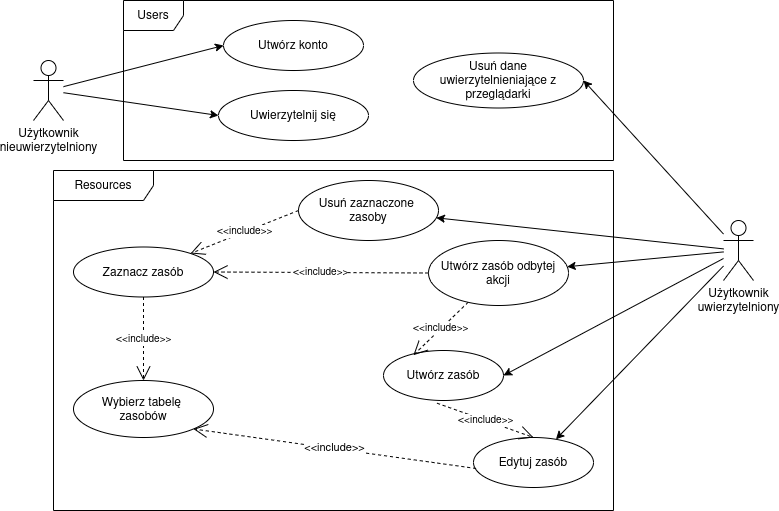
\includegraphics[width=\textwidth]{img/chapter4/open-osp.uml-diagrams-use-case.png}
    \caption{Diagram przypadków użycia}
    \label{fig:uml.use-case}
\end{figure}

%%%%%%%%%%%%%%%%%%%%%%%%%%%%%%%%%%%%%%%%%%%%%%%%%%%%%%%%%%%%%%%%%%%%%%%%%%%%%%%%
\section{Diagram klas encji}
%%%%%%%%%%%%%%%%%%%%%%%%%%%%%%%%%%%%%%%%%%%%%%%%%%%%%%%%%%%%%%%%%%%%%%%%%%%%%%%%

W celu zaprojektowania podstawowych struktur danych, biorących udział w procesach logicznych systemu, sklasyfikowano przechowywane w bazie danych encje:

\begin{itemize}
    \item User - obiekt opisujący konto założone przez użytkownika aplikacji. Zawiera atrybuty adresu e-mail, będącego identyfikatorem użytkownika w procesie uwierzytelniającym oraz zaszyfrowaną wersję hasła.
    \item Member - obiekt członka jednostki strażackiej mogącego brać udział w akcjach. W podstawowej wersji systemu, członek drużyny jest opisany przez atrybuty swojego imienia, nazwiska i numeru PESEL. W dalszym procesie rozwoju aplikacji, należałoby rozważyć dodanie atrybutów takich jak ranga, zdobyte odznaczenia czy termin następnych badań okresowych.
    \item Equipment - obiekt reprezentujący sprzęt, wchodzący w inwentarz jednostki, taki jak samochody, piły spalinowe lub węże strażackie. Dla uproszczenia tworzonego prototypu, zdecydowano się na jedną klasę opisującą użyteczne przedmioty, przy pomocy atrybutów nazwy własnej, marki, modelu i numeru seryjnego (pełniącego również rolę numerów rejestracyjnych dla pojazdów spalinowych). 
    \item Action - obiekt akcji strażackiej opisujący ją przy pomocy atrybutów jej typu i lokacji podanej przy pomocy szerokości oraz długości geograficznej. Każda z akcji będzie miała również swój czas rozpoczęcia i zakończenia.
    \item ActionMember - obiekt opisujący rolę danego członka zespołu w odbytej akcji. Jego atrybutami są unikalne numery identyfikujące członka jednostki oraz akcji, w której bierze on udział. Rola członka zespołu jest określana przy pomocy, przeznaczonego w tym celu typu wyliczeniowego.
    \item ActionEquipment - obiekt opisujący eksploatacje sprzętu  w odbytej akcji. Pierwszorzędnymi atrybutami encji są unikalne identyfikatory odbytej akcji oraz sprzętu strażackiego. Jego zużycie można opisać dodatkowo atrybutami ilości zużytych litrów paliwa oraz stanu licznika po akcji.
\end{itemize}

W procesie opisywania klas, wyodrębniono dodatkowe dwa typy numeryczne. Typy te pozwalają na bardziej klarowny sposób zarządzania informacjami zapisanymi przy pomocy pojedynczej liczby całkowitej:

\begin{itemize}
    \item ActionType - typ wyliczeniowy określający rodzaj odbytej akcji. Wśród możliwych wartości wyróżniono: wyjazd zaopatrzeniowy, akcję treningową, akcję pożarniczą i zwalczanie innych zagrożeń/klęsk żywiołowych.
    \item ActionMemberRole - określa rolę członka drużyny uczestniczącego w akcji. Członek drużyny może zostać rozróżniony jako: zwykły członek zespołu, kierowca lub dowódca.
\end{itemize}

Typy wyliczeniowe, stanowią bardzo pożyteczne narzędzie w programowaniu wysokopoziomowym, pozwalając na  oszczędność pamięci i ograniczenie złożoności obliczeniowej, względem typów takich jak łańcuch znaków. Zapewniają również, bardzo korzystną dla inżynierów oprogramowania, skalowalność tworzonego rozwiązania.

Stworzony na podstawie przeprowadzonej analizy, diagram klas UML został przedstawiony na rys. \ref{fig:uml.classes}. Stanowi on przejrzysty projekt warstwy modelu danych systemu, umożliwiając rozpoczęcie prac nad logiką biznesową. Diagramy klas stanowią najpopularniejsze diagramy UML, stosowane w inżynierii oprogramowania, należące do podzbioru diagramów strukturalnych.

\begin{figure}[!htbp]
    \centering
    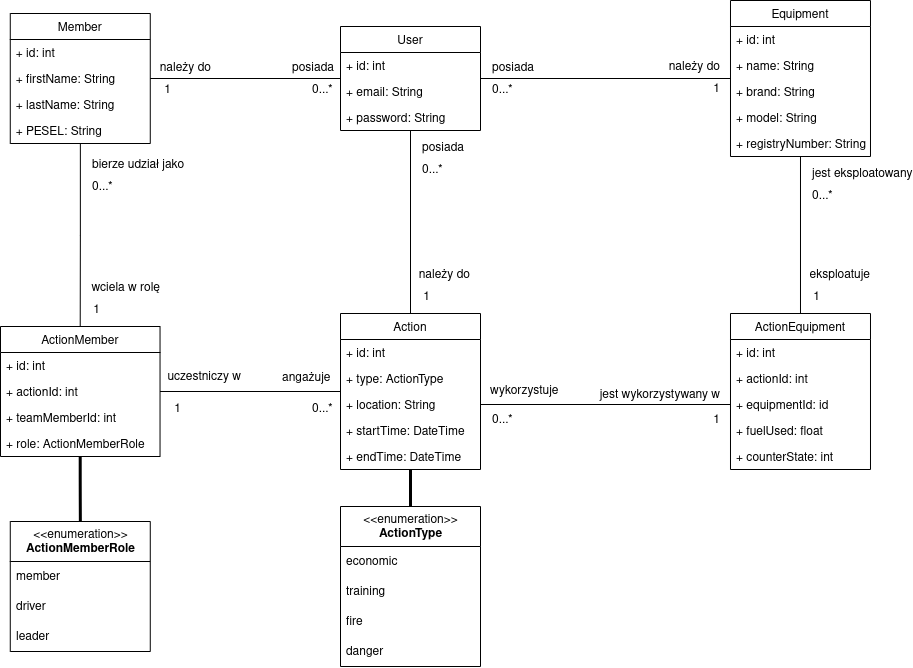
\includegraphics[width=\textwidth]{img/chapter4/open-osp.uml-diagrams-classes.png}
    \caption{Diagram klas encji}
    \label{fig:uml.classes}
\end{figure}

%%%%%%%%%%%%%%%%%%%%%%%%%%%%%%%%%%%%%%%%%%%%%%%%%%%%%%%%%%%%%%%%%%%%%%%%%%%%%%%%
\section{Diagram aktywności}
%%%%%%%%%%%%%%%%%%%%%%%%%%%%%%%%%%%%%%%%%%%%%%%%%%%%%%%%%%%%%%%%%%%%%%%%%%%%%%%%

Projektowanie warstwy logiki systemu, rozpoczęto od stworzenia diagramu aktywności. Diagram ten, stanowi jeden z najpopularniejszych sposobów, przedstawienia przebiegu interakcji między użytkownikiem, a oprogramowaniem. Jako przedstawiciel zbioru diagramów zachowań, jest powiązany z przedstawionym na rys. \ref{fig:uml.use-case} diagramem przypadków użycia, wyróżniając się dodatkowymi oznaczeniami dla podejmowanych decyzji i ciągłością przebiegu.

\begin{figure}[!htbp]
    \centering
    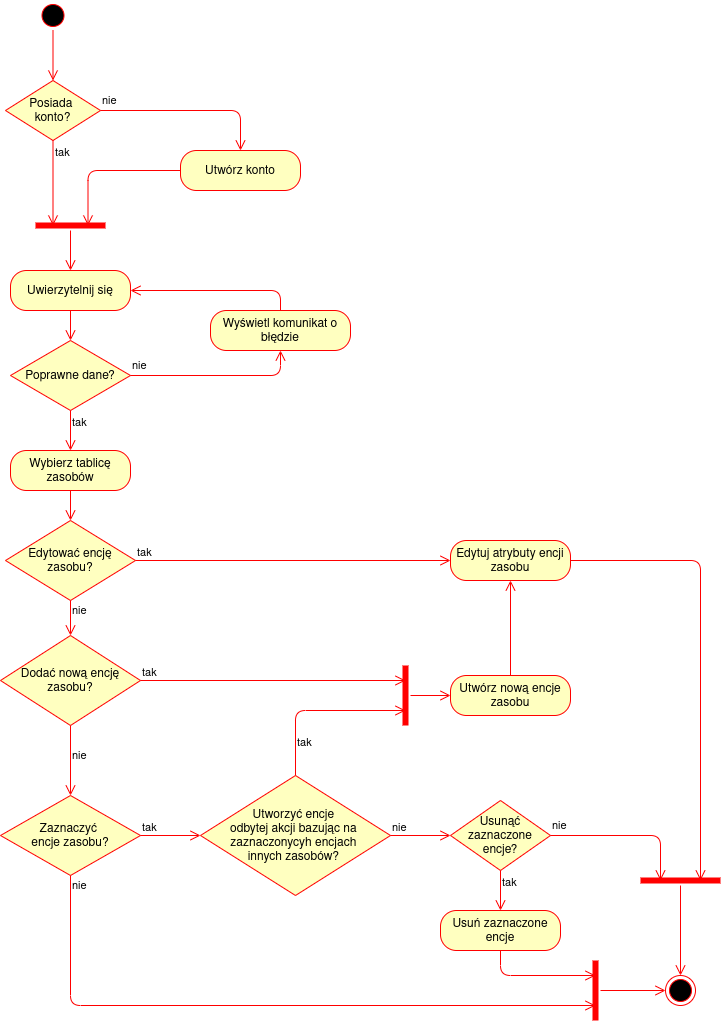
\includegraphics[width=\textwidth]{img/chapter4/open-osp.uml-diagrams-activity.png}
    \caption{Diagram aktywności}
    \label{fig:uml.activity}
\end{figure}

Diagram aktywności przedstawiony na rys. \ref{fig:uml.activity} jest szczególnie przydatny przy planowaniu ilości i przeznaczenia widoków w aplikacji klienckiej. W celu przedstawienia szczegółowego cyklu życia zasobów, przypisanych do użytkownika systemu, zastosowano diagramy sekwencji opisane w dalszej sekcji.

%%%%%%%%%%%%%%%%%%%%%%%%%%%%%%%%%%%%%%%%%%%%%%%%%%%%%%%%%%%%%%%%%%%%%%%%%%%%%%%%
\section{Widoki aplikacji klienckiej}
%%%%%%%%%%%%%%%%%%%%%%%%%%%%%%%%%%%%%%%%%%%%%%%%%%%%%%%%%%%%%%%%%%%%%%%%%%%%%%%%

Bazując na diagramie aktywności, wyróżniono widoki aplikacji, stanowiące interfejs między użytkownikiem, a dostarczanymi przez system funkcjonalnościami. Warstwę widoku aplikacji tworzą niżej opisane składowe:

\begin{itemize}
    \item Strona tytułowa aplikacji, zawierająca odnośniki do widoku uwierzytelnienia i rejestracji użytkowników.
    \item Widok formularza uwierzytelnienia, składającego się z pola do wprowadzenia e-maila oraz hasła użytkownika.
    \item Widok rejestracji użytkowników, zawierający formularz do wprowadzenia danych.
    \item Widok panelu użytkownika, umożliwiającego wybór przeglądanej tabeli zasobów. W jego skład wchodzi tabela, w której każda z krotek posiada pole zaznaczenia i przycisk edycji.
    \item Widok edycji atrybutów zasobu przy pomocy pojawiającego się monitu, jednocześnie pełni funkcję widoku służącego do inicjalizacji atrybutów nowo powstałej encji.
    \item Widok edycji encji odbytej akcji. Formularz rozbudowany jest o sekcje, pozwalające uzupełnić informacje o członkach drużyny i sprzęcie, który wziął udział w akcji.
    \item Widok ostrzeżenia przed usunięciem, zaznaczonych w tabeli zasobów.
\end{itemize}

\begin{figure}[!htbp]
\centering
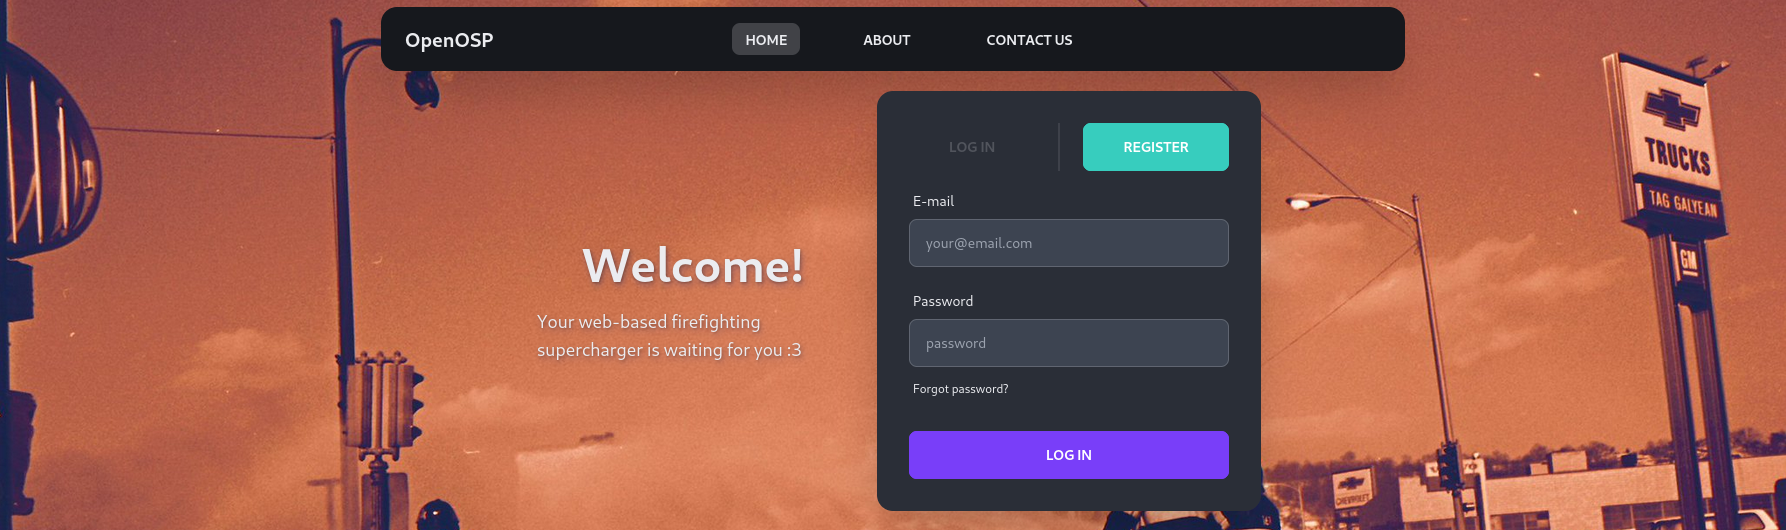
\includegraphics[width=\textwidth]{img/chapter4/views/login.png}
\caption{Widok formularza uwierzytelnienia użytkownika}
\end{figure}

\begin{figure}[!htbp]
\centering
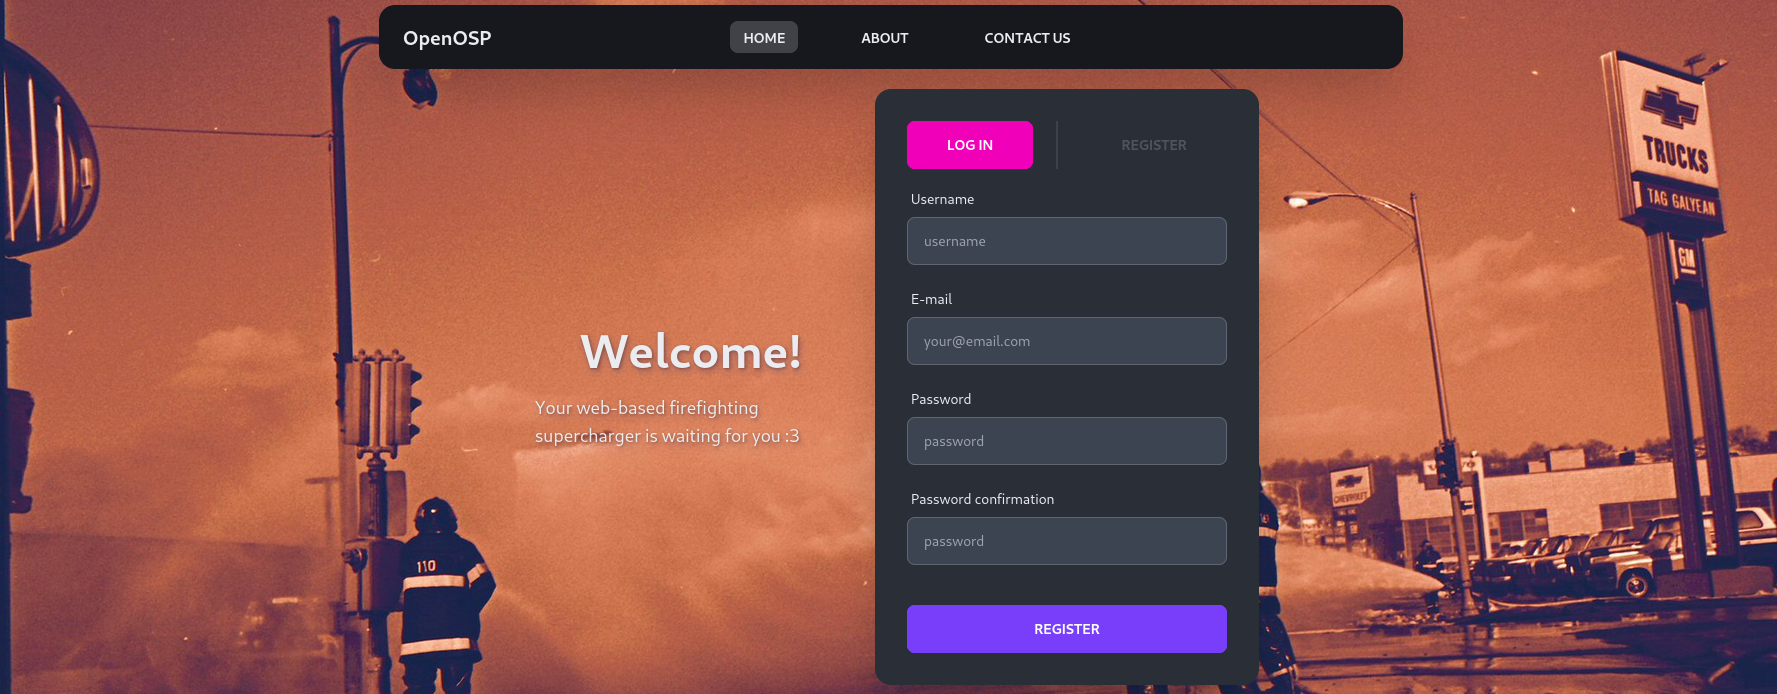
\includegraphics[width=\textwidth]{img/chapter4/views/registration.png}
\caption{Widok formularza rejestracji użytkownika}
\end{figure}

\begin{figure}[!htbp]
\centering
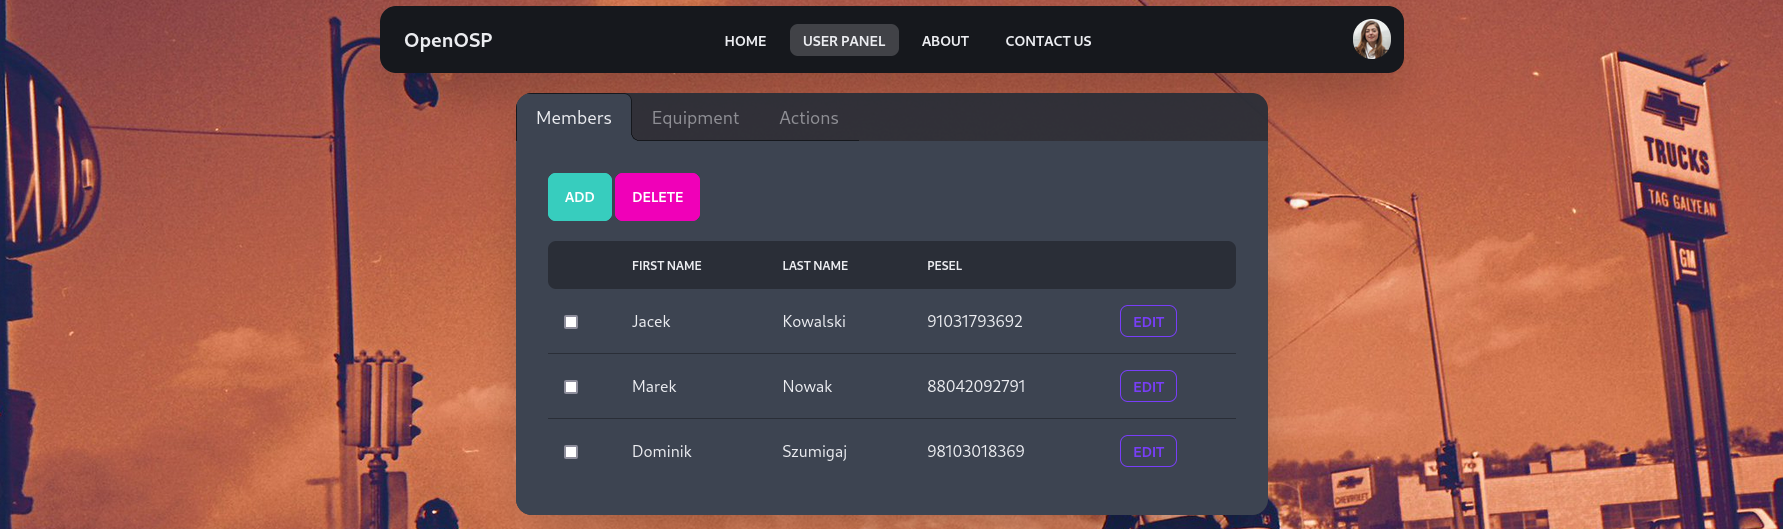
\includegraphics[width=\textwidth]{img/chapter4/views/userpanel.png}
\caption{Widok tabeli zasobów użytkownika}
\end{figure}

\begin{figure}[!htbp]
\centering
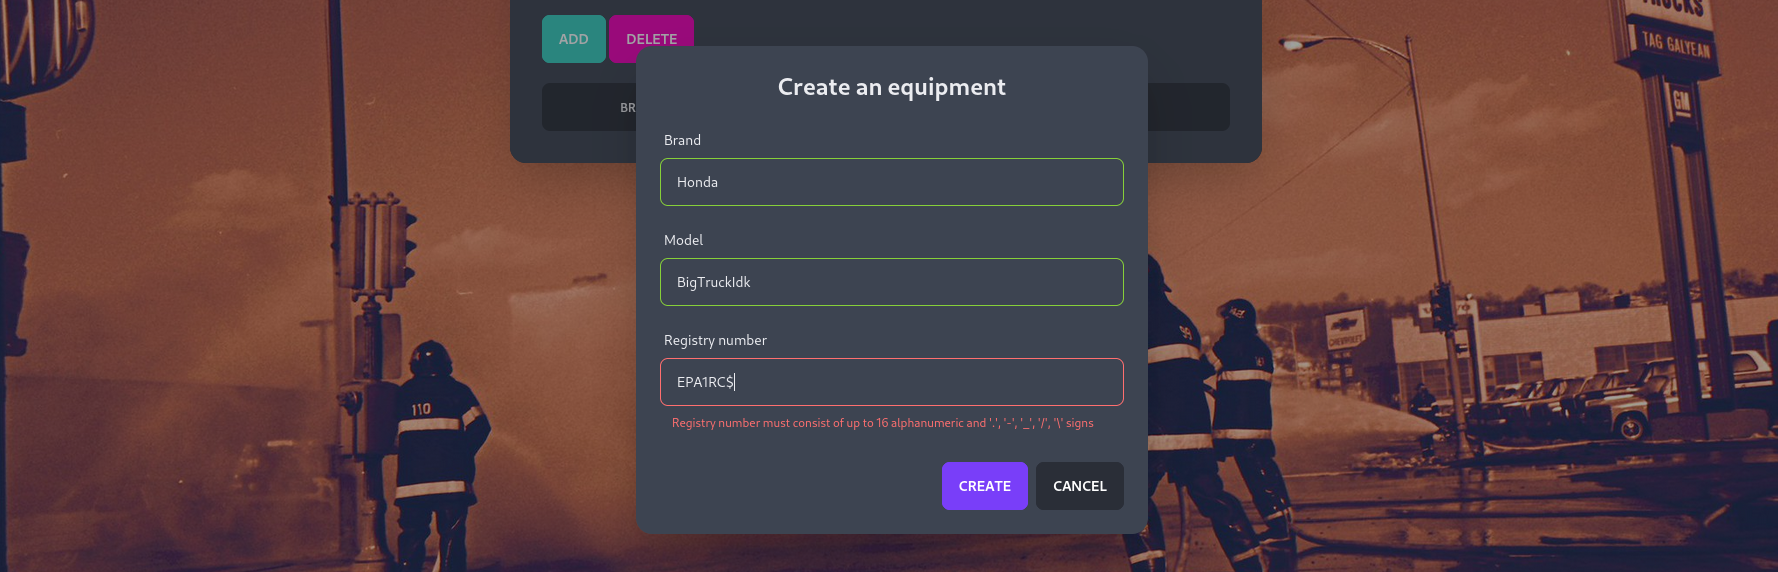
\includegraphics[width=\textwidth]{img/chapter4/views/create.png}
\caption{Widok monitu tworzenia lub modyfikacji zasobu}
\end{figure}

\begin{figure}[!htbp]
\centering

\includegraphics[width=\textwidth]{img/chapter4/views/action.png}
\caption{Widok monitu tworzenia lub modyfikacji zasobu odbytej akcji}
\end{figure}

\begin{figure}[!htbp]
\centering
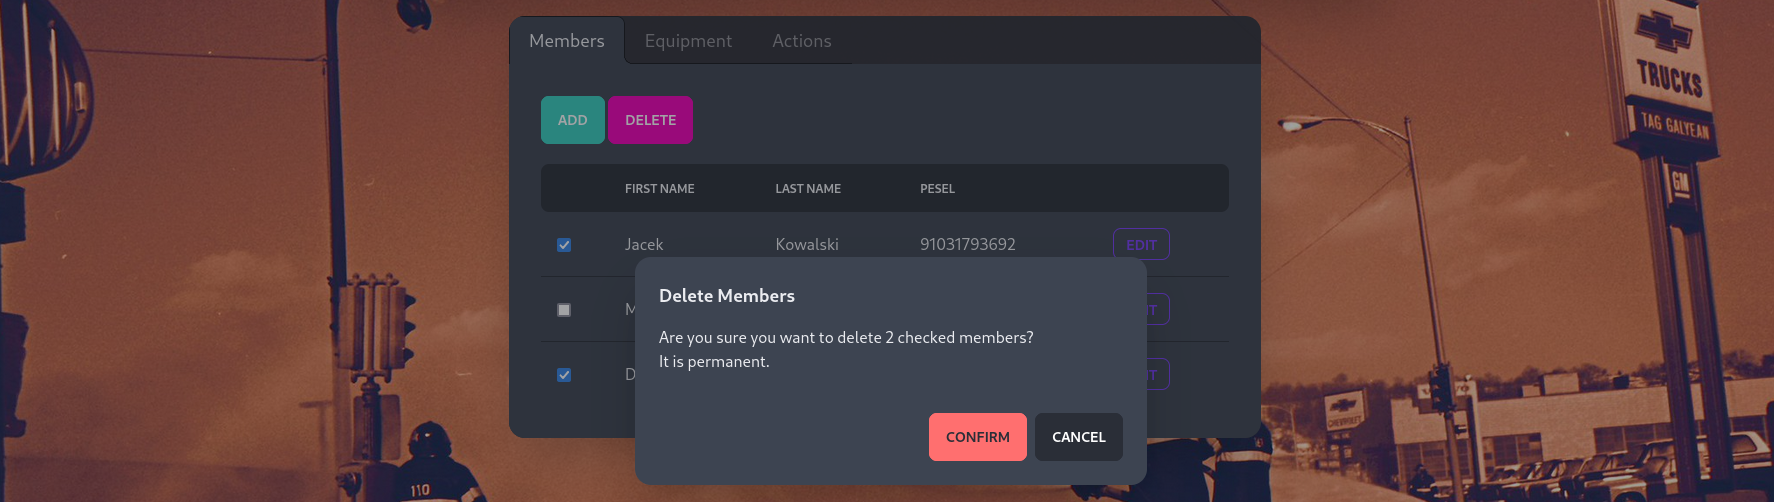
\includegraphics[width=\textwidth]{img/chapter4/views/delete.png}
\caption{Widok monitu ostrzeżenia przed usunięciem zasobów}
\end{figure}

W każdym z widoków, użytkownik ma dostęp do paska nawigacyjnego zawierającego odnośniki do panelu użytkownika oraz przycisk do wylogowania się z aplikacji. 

%%%%%%%%%%%%%%%%%%%%%%%%%%%%%%%%%%%%%%%%%%%%%%%%%%%%%%%%%%%%%%%%%%%%%%%%%%%%%%%%
\section{Cykl życia zasobu użytkownika}
%%%%%%%%%%%%%%%%%%%%%%%%%%%%%%%%%%%%%%%%%%%%%%%%%%%%%%%%%%%%%%%%%%%%%%%%%%%%%%%%

Procesy, związane z przetwarzaniem obiektów zasobów użytkownika, zostały wyodrębnione jako najważniejszy element logiczny tworzonego systemu. Z tego względu, użyto diagramów sekwencji przy projektowaniu tych funkcjonalności systemu.

Diagramy sekwencji, stanowią jedne z najbardziej szczegółowych diagramów zachowań UML, pozwalając na bardzo dokładny opis interakcji między elementami tworzonej infrastruktury. Zawdzięczają to zastosowaniu linii życia dla każdego z elementów oraz możliwości wykorzystania bloków zapętlonych lub warunkowych, okalających zbiory sygnałów, wymienianych między tymi elementami.

Sekcję ograniczono do trzech scenariuszy, odzwierciedlających przypadki użycia aplikacji. Jednakże, opisują one wystarczająco, zasadę działania warstwy logiki całego systemu.

%%%%%%%%%%%%%%%%%%%%%%%%%%%%%%%%%%%%%%%%
\subsection{Dodawanie zasobu użytkownika}
%%%%%%%%%%%%%%%%%%%%%%%%%%%%%%%%%%%%%%%%

Przebieg dodawania encji zasobu, przypisanego do użytkownika w systemie, został przedstawiony w diagramie na rys. \ref{fig:uml.sequence.create-resource} oraz opisany przy pomocy niżej zamieszczonego scenariusza.

\begin{figure}[!htbp] 
    \centering
    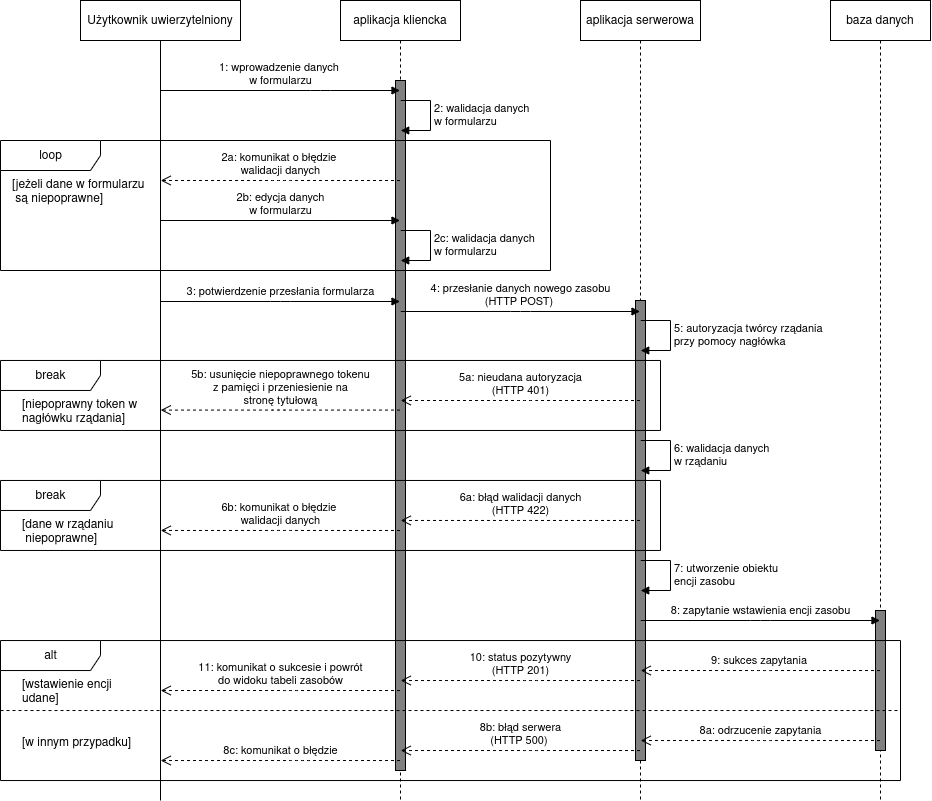
\includegraphics[width=\textwidth]{img/chapter4/open-osp.uml-diagrams-sequence.create-resource.png}
    \caption{Diagram sekwencji dodawania zasobu użytkownika}
    \label{fig:uml.sequence.create-resource}
\end{figure}

Jedynym aktorem, występującym w procesie, jest użytkownik uwierzytelniony, który dodaje przypisaną do niego encje zasobu w systemie. Warunkiem wstępnym jest, aby użytkownik korzystał od początku z widoku tworzenia nowego zasobu i posiadał token autoryzacyjny. Za warunek końcowy scenariusza, uznano sytuację, w której nowy zasób przypisany do użytkownika, został dodany do bazy danych systemu, a sam użytkownik został o tym fakcie poinformowany.

Główny przebieg zdarzeń opisany został w następującej kolejności:

\begin{enumerate}
    \item Użytkownik wprowadza w polach formularza tworzenia nowego zasobu, wartości jego atrybutów, wykorzystując aplikację kliencką.
    \item Aplikacja kliencka w sposób dynamiczny dokonuje walidacji danych w formularzu.
    \item Użytkownik potwierdza dodanie nowego zasobu przy pomocy przycisku przesłania formularza.
    \item Aplikacja kliencka wysyła żądanie HTTP metodą POST do interfejsu programistycznego aplikacji serwerowej. Żądanie zawiera dane nowego zasobu do utworzenia oraz token autoryzacyjny w nagłówku.
    \item Aplikacja serwerowa autoryzuje twórcę żądania przy pomocy przesłanego tokenu, sprawdzając między innymi jego ważność.
    \item Aplikacja serwerowa przeprowadza procedurę walidacji danych przesłanych w żądaniu.
    \item Aplikacja serwerowa tworzy obiekt encji zasobu, który zostanie zarejestrowany przez mechanizm mapowania obiektowo-relacyjnego.
    \item Aplikacja serwerowa przesyła do bazy danych zapytanie utworzenia nowej krotki w tabeli zasobów.
    \item W odpowiedzi baza danych przesyła komunikat o sukcesie zapytania.
    \item Aplikacja serwerowa wysyła do aplikacji klienckiej odpowiedź HTTP ze statusem 201, świadczącym o pomyślnym utworzeniu encji zasobu.
    \item Aplikacja kliencka informuje użytkownika o udanym utworzeniu przypisanego do niego zasobu.
\end{enumerate}

Wyróżniony został zakres zdarzeń opcjonalnych dla przypadku, w którym walidacja danych w kroku 2, wykryła niepoprawne dane wprowadzone w formularzu:

\begin{enumerate}
    \item [2a.] Aplikacja kliencka wyświetla komunikat o niepoprawnych danych wprowadzonych w formularzu.
    \item [2b.] Użytkownik edytuje dane w formularzu.
    \item [2c.] Aplikacja kliencka ponownie dokonuje walidacji danych. Jeżeli wprowadzone dane ponownie są niepoprawne, powtórzone zostaną zdarzenia 2a, 2b i 2c.
\end{enumerate}

W scenariuszu uwzględniono również niżej przedstawione zdarzenia alternatywne:

\begin{enumerate}
    \item [5a.] Ze względu na błąd autoryzacji, aplikacja serwerowa przesyła do aplikacji klienckiej odpowiedź HTTP ze statusem 401 (brak autoryzacji).
    \item [5b.] Aplikacja kliencka usuwa niepoprawny token z pamięci przeglądarki użytkownika i przenosi go do widoku strony tytułowej.
    \item [6a.] Aplikacja serwerowa wysyła do aplikacji klienckiej odpowiedź HTTP ze statusem 422 (niewykonalne żądanie).
    \item [6b.] Aplikacja kliencka informuje użytkownika o błędzie i prosi o ponowne uzupełnienie formularza.
    \item [8a.] Baza danych informuje o odrzuceniu zapytania utworzenia encji lub nie odpowiada aplikacji serwerowej. 
    \item [8b.] Aplikacja serwerowa przesyła aplikacji klienckiej informacje o błędzie wewnętrznym serwera przy pomocy odpowiedzi HTTP 500. 
    \item [8c.] Aplikacja kliencka informuje użytkownika o nieudanej obsłudze żądania.
\end{enumerate}

%%%%%%%%%%%%%%%%%%%%%%%%%%%%%%%%%%%%%%%%
\subsection{Edycja zasobu użytkownika}
%%%%%%%%%%%%%%%%%%%%%%%%%%%%%%%%%%%%%%%%

Proces edycji zasobu użytkownika zobrazowano diagramem na rys. \ref{fig:uml.sequence.update-resource}. Jedynym aktorem występującym w scenariuszu jest użytkownik uwierzytelniony. Zgodnie z warunkiem wstępnym, użytkownik na początku scenariusza korzysta z widoku edycji zasobu. Warunkiem końcowym jest, aby atrybuty edytowanego zasobu, zostały zaktualizowane w bazie danych systemu i użytkownik otrzymał komunikat o pomyślnie przeprowadzonej akcji.

\begin{figure}[!htbp] 
    \centering
    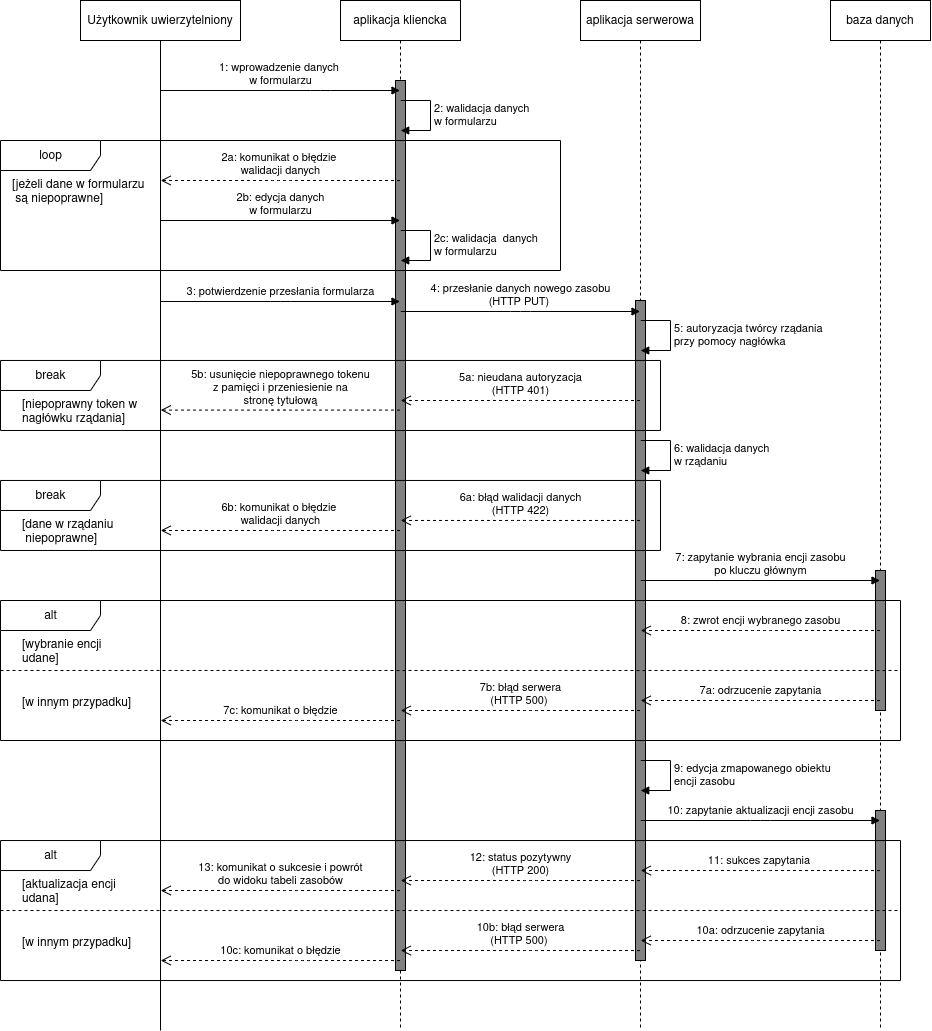
\includegraphics[width=\textwidth]{img/chapter4/open-osp.uml-diagrams-sequence.update-resource.png}
    \caption{Diagram sekwencji edycji zasobu}
    \label{fig:uml.sequence.update-resource}
\end{figure}

Poniżej wypunktowano główny przebieg zdarzeń scenariusza:

\begin{enumerate}
    \item Użytkownik wprowadza w polach formularza edycji zasobu, wartości jego atrybutów wykorzystując aplikację kliencką.
    \item Aplikacja kliencka w sposób dynamiczny dokonuje walidacji danych w formularzu.
    \item Użytkownik potwierdza edycje zasobu przy pomocy przycisku przesłania formularza.
    \item Aplikacja kliencka wysyła żądanie HTTP metodą PUT do interfejsu programistycznego aplikacji serwerowej. Żądanie zawiera nowe dane edytowanego zasobu oraz token autoryzujący w nagłówku.
    \item Aplikacja serwerowa autoryzuje twórcę żądania przy pomocy przesłanego tokenu.
    \item Aplikacja serwerowa przeprowadza procedurę walidacji danych przesłanych w żądaniu.
    \item Aplikacja serwerowa wysyła do bazy danych zapytanie wybrania istniejącej encji po kluczu głównym.
    \item Baza danych zwraca krotkę zasobu w odpowiedzi na zapytanie aplikacji serwerowej.
    \item Aplikacja serwerowa modyfikuje atrybuty encji poprzez edycje obiektu monitorowanego przez mechanizm obiektowo-relacyjny.
    \item Aplikacja serwerowa przesyła do bazy danych zapytanie aktualizacji krotki encji w tabeli zasobów.
    \item W odpowiedzi baza danych przesyła komunikat o sukcesie zapytania.
    \item Aplikacja serwerowa wysyła do aplikacji klienckiej odpowiedź HTTP z pozytywnym statusem 200. 
    \item Aplikacja kliencka informuje użytkownika o udanej modyfikacji zasobu.
\end{enumerate}

Jeżeli użytkownik wprowadził niepoprawne dane w formularzu, walidacja danych w kroku 2 nie powiedzie się, skutkując wystąpieniem opcjonalnych zdarzeń:

\begin{enumerate}
    \item [2a.] Aplikacja kliencka wyświetla komunikat o niepoprawnych danych wprowadzonych w formularzu.
    \item [2b.] Użytkownik edytuje dane w formularzu.
    \item [2c.] Aplikacja kliencka ponownie dokonuje walidacji danych. Jeżeli wprowadzone dane ponownie są niepoprawne, powtórzone zostaną zdarzenia 2a, 2b i 2c.
\end{enumerate}

Zdarzenia alternatywne, które mogą wystąpić w procesie edycji zasobu to:

\begin{enumerate}
    \item [5a.] Ze względu na błąd autoryzacji, aplikacja serwerowa przesyła do aplikacji klienckiej odpowiedź HTTP ze statusem 401 (brak autoryzacji).
    \item [5b.] Aplikacja kliencka usuwa niepoprawny token z pamięci przeglądarki użytkownika i przenosi go do widoku strony tytułowej.
    \item [6a.] Aplikacja serwerowa wysyła do aplikacji klienckiej odpowiedź HTTP ze statusem 422 (niewykonalne żądanie).
    \item [6b.] Aplikacja kliencka informuje użytkownika o błędzie i prosi o ponowne uzupełnienie formularza.
    \item [7a.] Baza danych informuje o odrzuceniu zapytania wybrania encji lub nie odpowiada aplikacji serwerowej. 
    \item [7b.] Aplikacja serwerowa przesyła aplikacji klienckiej informacje o błędzie wewnętrznym serwera przy pomocy odpowiedzi HTTP 500. 
    \item [7c.] Aplikacja kliencka informuje użytkownika o nieudanej obsłudze żądania.
    \item [10a.] Baza danych informuje o odrzuceniu zapytania aktualizacji encji lub nie odpowiada aplikacji serwerowej. 
    \item [10b.] Aplikacja serwerowa przesyła aplikacji klienckiej informacje o błędzie wewnętrznym serwera przy pomocy odpowiedzi HTTP 500. 
    \item [10c.] Aplikacja kliencka informuje użytkownika o nieudanej obsłudze żądania.
\end{enumerate}

%%%%%%%%%%%%%%%%%%%%%%%%%%%%%%%%%%%%%%%%
\subsection{Usuwanie zasobów użytkownika}
%%%%%%%%%%%%%%%%%%%%%%%%%%%%%%%%%%%%%%%%

Procedurę usuwania zasobów użytkownika zilustrowano przy pomocy diagramu sekwencji przedstawionego na rys. \ref{fig:uml.sequence.delete-resource}.

\begin{figure}[!htbp] 
    \centering
    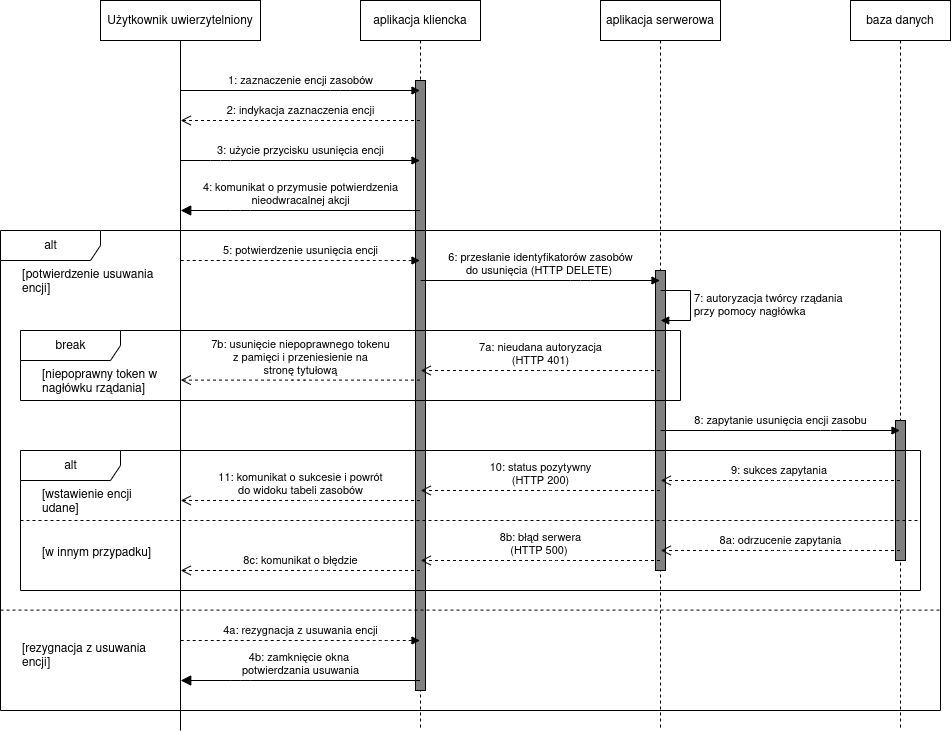
\includegraphics[width=\textwidth]{img/chapter4/open-osp.uml-diagrams-sequence.delete-resource.png}
    \caption{Diagram sekwencji usuwania zasobu}
    \label{fig:uml.sequence.delete-resource}
\end{figure}

Jedynym aktorem występującym w procesie jest użytkownik uwierzytelniony. Użytkownik wstępnie posiada token autoryzujący zapisany w pamięci przeglądarki i korzysta z widoku tabeli zasobów. Warunkiem końcowym jest natomiast trwałe usunięcie zasobu z bazy danych systemu.

Główny przebieg zdarzeń opisany został w następującej kolejności:

\begin{enumerate}
    \item Użytkownik zaznacza zasoby przy pomocy interfejsu aplikacji klienckiej.
    \item Aplikacja kliencka wyraźnie indykuje zaznaczenie zasobów.
    \item Użytkownik korzysta z przycisku usunięcia zaznaczonych zasobów.
    \item Aplikacja kliencka wyświetla widok potwierdzenia nieodwracalnego usunięcia zasobów.
    \item Użytkownik potwierdza zamiar usunięcia zaznaczonych zasobów.
    \item Aplikacja kliencka wysyła żądanie HTTP metodą DELETE do interfejsu programistycznego aplikacji serwerowej. Żądanie zawiera unikalne identyfikatory zasobów do usunięcia oraz token autoryzujący w nagłówku.
    \item Aplikacja serwerowa autoryzuje twórcę żądania przy pomocy przesłanego tokenu, sprawdzając między innymi jego ważność.
    \item Aplikacja serwerowa wysyła zapytanie usunięcia zasobów o przesłanych w żądaniu identyfikatorach.
    \item W odpowiedzi baza danych przesyła komunikat o sukcesie zapytania.
    \item Aplikacja serwerowa wysyła do aplikacji klienckiej odpowiedź HTTP ze statusem 200 świadczącym o pomyślnym skasowaniu zasobów z pamięci.
    \item Aplikacja kliencka informuje użytkownika o udanym usunięciu zasobów.
\end{enumerate}

Jako dopuszczalne zdarzenia alternatywne traktuje się:

\begin{enumerate}
    \item [7a.] Ze względu na błąd autoryzacji, aplikacja serwerowa przesyła do aplikacji klienckiej odpowiedź HTTP ze statusem 401 (brak autoryzacji).
    \item [7b.] Aplikacja kliencka usuwa niepoprawny token z pamięci przeglądarki użytkownika i przenosi go do widoku strony tytułowej.
    \item [8a.] Baza danych informuje o odrzuceniu zapytania usunięcia encji lub nie odpowiada aplikacji serwerowej. 
    \item [8b.] Aplikacja serwerowa przesyła aplikacji klienckiej informacje o błędzie wewnętrznym serwera, przy pomocy odpowiedzi HTTP 500. 
    \item [8c.] Aplikacja kliencka informuje użytkownika o nieudanej obsłudze żądania.
\end{enumerate}

\chapter{Proces implementacji}
%%%%%%%%%%%%%%%%%%%%%%%%%%%%%%%%%%%%%%%%%%%%%%%%%%%%%%%%%%%%%%%%%%%%%%%%%%%%%%%%
\section{Zastosowane technologie}
%%%%%%%%%%%%%%%%%%%%%%%%%%%%%%%%%%%%%%%%%%%%%%%%%%%%%%%%%%%%%%%%%%%%%%%%%%%%%%%%

Rozdział 5 zawiera opis użytych w tej pracy narzędzi. Ze względu na fakt największej styczności z platformą programistyczną .NET oraz językiem C\#, w tworzonym rozwiązaniu, skorzystano ze stosunkowo mniej popularnych zbiorów bibliotek.

Wszystkie projekty składające się na system, zostały zaimplementowane w języku programowania C\# oraz z wykorzystaniem platformy .NET w wersji 6.0.100. Jest to produkt konkurencyjny do technologii Java, jednakże działają w podobny sposób. Platforma wykorzystuje możliwości kompilowania języków programowania takich jak C\# i F\#  do dwóch wersji. Pierwsza, binarna jest dedykowana do konkretnej platformy np. Windows x64.  Drugi wariant kompiluje program do języka pośredniego, umożliwiającego  uruchomienie tworzonych rozwiązań na wszystkich platformach, na których istnieje implementacja odpowiedniej wersji środowiska uruchomieniowego .NET.

Najważniejszym dla systemów internetowych podzbiorem bibliotek platformy, są aktywne strony serwera .NET (ASP.NET Core). Dzięki swej modularności, może on służyć do stworzenia większości rodzajów aplikacji chmurowych, w sposób zapewniający im odpowiednią skalowalność oraz łatwe tworzenie testów:

\begin{itemize}
    \item Webowe interfejsy aplikacyjne (Web API) - aplikacje serwerowe, zapewniające funkcjonalność znaną ze stylów architektonicznych takich jak REST czy nowszy GraphQL. 
    \item Aplikacje chmurowe z dziedziny Internetu Rzeczy (IoT), pozwalające na łatwą manipulację danymi w systemach rozproszonych.
    \item Serwisy i mikroserwisy gRPC, stanowiące minimalistyczną i wydajną alternatywę do obarczonych większą ilością przesyłanych metadanych, webowych interfejsów aplikacyjnych.
    \item Aplikacje Model-View-Controler (MVC), wykorzystujące autorskie rozwiązanie języka znaczników Razor, jako pliki *.cshtml widoków. Razor umożliwia wykorzystanie standardowych znaczników HTML w połączeniu z logiką języka C\#. Źródłem logiki interfejsu użytkownika, są w tych aplikacjach kontrolery, odpowiedzialne również za komunikację z klasami modelu zarządzającymi danymi aplikacji.
    \item Aplikacje stron Razor (Razor Pages), w których logika związana z interfejsem użytkownika, została przeniesiona z klas kontrolerów do dedykowanych dla stron *.cshtml (opcjonalnych) plików *.cshtml.cs bedących, zwykłymi klasami języka C\#.
    \item Aplikacje Blazor, stanowiące najbardziej nowoczesny sposób tworzenia internetowych aplikacji klienckich. Platforma Blazor rozbudowuje zadania języka znaczników Razor do tworzenia całych komponentów w plikach *.razor. W odróżnieniu od architektury MVC oraz stron Razor, aplikacje te świadczą usługi aplikacji pojedynczej strony (SPA). Jest to sposób działania, znany z nowoczesnych aplikacji klienckich, tworzonych przy pomocy platform takich jak Angular, React czy Vue. Blazor odróżnia się jednak tym, że wykorzystuje w logice komponentów język C\# zamiast języka JavaScript.
\end{itemize}

Jednym z najbardziej rozpoznawalnych rozwiązań, wykorzystywanych w parze z platformą ASP.NET Core, jest dedykowane jej narzędzie mapera obiektowo-relacyjnego o nazwie Entity Framework Core (EF Core). Dzięki bardzo wygodnemu narzędziu konsolowemu platformy .NET, umożliwia on bardzo szybkie rozpoczęcie pracy na jeden z trzech sposobów, zdefiniowanych w sekcji 3.11 poświęconej narzędziom ORM.

Dodatkowym i stosunkowo niestandardowym narzędziem, w stosie technologicznym platformy .NET, jest otwarto-źródłowy menadżer pakietów Paket. Stanowi on substytut, do domyślnego narzędzia Nuget, pozwalający na większą dozę współdzielenia pakietów zewnętrznych bibliotek między projektami.

Jako silnik bazy danych, wybrano narzędzie PostgreSQL (znane również jako Postgres), będące jednym z najpopularniejszych tego typu rozwiązań na rynku, obok oprogramowania MySQL czy SQL Server. Postgres stanowi, zdecydowanie najmocniej wspierany przez społeczność akademicką, projekt otwarto-źródłowego silnika relacyjnych baz danych, skrupulatnie rozwijany i dokumentowany już od lat 90-tych XX wieku. W ostatnich latach, zyskuje nawet nowe funkcjonalności związane z przechowywaniem danych w formacie JSON, mające zapewnić mu konkurencyjność względem rozwiązań NoSQL.

Platforma NodeJS stanowi praktycznie nierozłączny element tworzenia aplikacji internetowych w dzisiejszych czasach. W przypadku projektu, opisywanego w pracy, została użyta w celu importowania pakietów JS, wykorzystywanych przez aplikację kliencką oraz sformułowania pojedynczych skryptów pomocnych w budowaniu rozwiązania.

Kolejnym elementem, składającym się na technologie wykorzystywane w projekcie, jest platforma Tailwind CSS. Jako otwarto-źródłowy produkt generujący klasy CSS, poświęcone konkretnym deklaracjom, umożliwia rezygnację z wykorzystania osobnych arkuszy stylów CSS, podnosząc czytelność komponentów projektu. Przyczynia się również do znacznego przyśpieszania powstawania prototypów aplikacji.

%%%%%%%%%%%%%%%%%%%%%%%%%%%%%%%%%%%%%%%%%%%%%%%%%%%%%%%%%%%%%%%%%%%%%%%%%%%%%%%%
\section{Projekty składające się na rozwiązanie}
%%%%%%%%%%%%%%%%%%%%%%%%%%%%%%%%%%%%%%%%%%%%%%%%%%%%%%%%%%%%%%%%%%%%%%%%%%%%%%%%

Na rozwiązanie systemu internetowego OpenOsp, tworzonego w pracy, złożyły się trzy projekty platformy .NET, dzielące między sobą konkretne zadania:

\begin{itemize}
    \item OpenOsp.Client - projekt aplikacji klienckiej wykorzystującej platfomę Blazor z modelem hostingu WebAssembly. Aplikacja zostaje pobrana w całości do pamięci przeglądarki użytkownika, w postaci binarnej i działa w pełni po stronie klienta, w sposób opisany w sekcji 3.6, poświęconej standardowi WASM. W realnym scenariuszu, umożliwia to odciążenie serwerów dostawcy usługi i m.in. oszczędność na sprzęcie.
    \item OpenOsp.Server - projekt aplikacji serwerowej odwzorowującej architekturę webowych interfejsów REST. Aplikacja wykorzystuje bibliotekę EF Core, definiując kontekst bazy danych i konfigurację poszczególnych relacji, w dedykowanych ku temu plikach. Można go uznać za główny projekt rozwiązania, ze względu na fakt serwowania usług aplikacji klienckiej przy pomocy referencji do projektu OpenOsp.Client.
    \item OpenOsp.Model - projekt biblioteki klas, składający w sobie klasy zasobów wykorzystywane przez ORM systemu, ich reprezentacje w postaci obiektów transferu danych (DTO) oraz definicje adnotacji umożliwiających łatwą walidację danych. Obydwa projekty, OpenOsp.Client i OpenOsp.Server, wykorzystują referencje do tego projektu, unikając niepotrzebnych powtórzeń w kodzie.
\end{itemize}

Przykłady implementacji funkcjonalności i opis poszczególnych części rozwiązania, zostały zawarte w kolejnych sekcjach rozdziału.

%%%%%%%%%%%%%%%%%%%%%%%%%%%%%%%%%%%%%%%%%%%%%%%%%%%%%%%%%%%%%%%%%%%%%%%%%%%%%%%%
\section{Biblioteka klas zasobów i ich reprezentacji}
%%%%%%%%%%%%%%%%%%%%%%%%%%%%%%%%%%%%%%%%%%%%%%%%%%%%%%%%%%%%%%%%%%%%%%%%%%%%%%%%

Najważniejszym katalogiem w projekcie modelu jest Models, zbierający klasy reprezentujące zasoby w aplikacji serwerowej, używane do tworzenia relacji w bazie danych. Katalogi we wszystkich projektach, segregują najczęściej poszczególne przestrzenie nazw, przykładowo OpenOsp.Model.Models dla klas zasobów.

\begin{lstlisting}[language=CSharp, caption=Przykładowa klasa zasobu, label=lst:member]
using System.Collections.Generic;
using System.ComponentModel.DataAnnotations;
using System.ComponentModel.DataAnnotations.Schema;
using OspDA = OpenOsp.Model.DataAnnotations;

namespace OpenOsp.Model.Models; 

public class Member : IHasId<int>, IOwnedBy<int> {
  [Display(Name = "First name")]
  [OspDA.Required]
  [OspDA.MaxLength(24)]
  [OspDA.Name]
  public string FirstName { get; set; }

  [Display(Name = "Last name")]
  [OspDA.Required]
  [OspDA.MaxLength(24)]
  [OspDA.Name]
  public string LastName { get; set; }

  [Display(Name = "PESEL")]
  [Column(TypeName = "char(11)")]
  [OspDA.Required]
  [OspDA.MaxLength(11)]
  [OspDA.Pesel]
  public string Pesel { get; set; }

  public virtual User User { get; set; }

  public virtual IEnumerable<ActionMember> Actions { get; set; }

  [Key] [OspDA.Required] public int Id { get; set; }

  [Display(Name = "Member owner's id")]
  [Column("OwnerId")]
  [OspDA.Required]
  public int UserId { get; set; }
}
\end{lstlisting}

Przykładowa klasa zasobu została pokazana na listingu \ref{lst:member}. Oprócz publicznych pól, z metodami dostępu, reprezentujących kolumny w tabeli, klasa posiada dwa pola wirtualne. Mogą one służyć do tworzenia zapytań pobierających z bazy danych nie tylko poszczególną encję, ale również te połączone z nią relacją jeden-do-wielu lub jeden-do-jednego. Przykładowo, w ramach zapytania wybierającego z bazy danych członka zespołu, możliwe byłoby również wybranie użytkownika będącego jego właścicielem oraz encji reprezentujących wszystkie akcje, w których brał udział.

\begin{lstlisting}[language=CSharp, caption={Interfejs implementowany przez klasy zasobu, posiadające klucz główny lub klucz złożony}, label=lst:hasId]
public interface IHasId<T>
  where T : IEquatable<T>, IComparable<T> {
  T Id { get; set; }
}

public interface IHasId<T, T2> : IHasId<T>
  where T : IEquatable<T>, IComparable<T>
  where T2 : IEquatable<T2>, IComparable<T2> {
  T2 Id2 { get; set; }
}
\end{lstlisting}

Ważną rolę w systemie pełnią interfejsy pokazane na listingach \ref{lst:hasId} oraz \ref{lst:ownedBy}. Pierwszy z nich implementowany jest przez klasy zasobów, identyfikowanych przez klucz główny lub klucz złożony. Interfejsy zastrzegają dodatkowo, że typy stosowanych kluczy, muszą implementować komparatory (interfejsy IEquatable oraz IComparable), pozwalające na porównywanie ich z wartościami tego samego typu. Dzięki funkcjonalnościom interfejsów, jest możliwe m.in tworzenie zapytań do bazy danych, przeszukujących rekordy tabeli po ich kluczach.

\begin{lstlisting}[language=CSharp, caption={Interfejs implementowany przez klasy zasobów, będących w relacji wiele-do-jednego z encją ich właściciela, identyfikowanego przez klucz główny}, label=lst:ownedBy]
public interface IOwnedBy<TUserId>
  where TUserId : IEquatable<TUserId>, IComparable<TUserId> {
  [OspDA.Required] public TUserId UserId { get; set; }
}
\end{lstlisting}

Interfejs IOwnedBy jest implementowany przez klasy zasobów, znajdujących się w relacji wiele-do-jednego ze swoim właścicielem. Ich właścicielem w systemie jest encja użytkownika, posiadająca własny klucz główny. Jednakże, dzięki zastosowaniu interfejsu, ponownie można użyć go w innych generycznych klasach systemu. W tym przypadku, będzie to automatyczne wprowadzenie klucza użytkownika do odpowiedniego atrybutu zasobu, przy jego tworzeniu oraz wykorzystanie deklarowanego klucza w mechanizmie autoryzacji per-wiersz.

Innym ważnym elementem klas zasobów są adnotacje danych, przypisane do konkretnych pól. Niektóre z nich takie jako Key i Column służą do określenia, czy dane pole klasy reprezentuje klucz główny oraz określenia nazwy i typu kolumny w tabeli. Inne można wykorzystać przy walidacji danych. Wówczas wartość pól, jest sprawdzana względem narzuconych im warunków, a w przypadku niepowodzenia, zwrócony zostanie stosowny komunikat o błędzie.

\begin{lstlisting}[language=CSharp, caption=Przykładowa klasa adnotacji danych, label=lst:name_attribute]
using System.ComponentModel.DataAnnotations;

namespace OpenOsp.Model.DataAnnotations; 

public class NameAttribute : RegularExpressionAttribute {
  public NameAttribute() : base(@"^[\p{L} \.\-]+$") {
    ErrorMessage = @"{0} is not a valid name";
  }
}
\end{lstlisting}

Przykładowo, na listingu \ref{lst:name_attribute} przedstawiono adnotację danych NameAttribute, służącą walidacji pól łańcuchów znaków, przy pomocy zdefiniowanego wyrażenia regularnego (regex). Wszystkie zdefiniowane podczas tworzenia systemu adnotacje danych, zostały zawarte w katalogu DataAnnotations i poświęconej im przestrzeni nazw OpenOsp.Model.DataAnnotations. 

W przypadku nieudanej walidacji, zostanie użyty komunikat o błędzie zdefiniowany w konstruktorze. W miejsce znacznika "{0}" wstawiona zostanie wizualna nazwa pola. Nazwa pola może zostać ustawiona ręcznie przy pomocy adnotacji Display, tak jak zostało to pokazane na listingu \ref{lst:member}.

Ważnym elementem w strukturze projektu jest katalog Dtos, zrzeszający pod jedną przestrzenią nazw, obiekty transferu danych będące m.in. reprezentacjami zasobów w systemie. Zawiera w sobie zarówno klasy obiektów, jak i klasy tzw. maperów tworzących obiekty zasobów, z obiektów ich reprezentacji i na odwrót.

\begin{lstlisting}[language=CSharp, caption={Przykładowa klasa obiektu transferu danych, stanowiąca reprezentację odczytu zasobu}, label=lst:member_read_dto]
using System.ComponentModel.DataAnnotations;
using OspDA = OpenOsp.Model.DataAnnotations;

namespace OpenOsp.Model.Dtos; 

public class MemberReadDto {
  [OspDA.Required] public int Id { get; set; }

  [Display(Name = "First name")]
  [OspDA.Required]
  [OspDA.MaxLength(24)]
  [OspDA.Name]
  public string FirstName { get; set; }

  [Display(Name = "Last name")]
  [OspDA.Required]
  [OspDA.MaxLength(24)]
  [OspDA.Name]
  public string LastName { get; set; }

  [Display(Name = "PESEL")]
  [OspDA.Required]
  [OspDA.Pesel]
  public string Pesel { get; set; }
}
\end{lstlisting}

\begin{lstlisting}[language=CSharp, caption={Przykładowa klasa obiektu transferu danych, stanowiąca reprezentację aktualizacji zasobu}, label=lst:member_update_dto]
using System.ComponentModel.DataAnnotations;
using OspDA = OpenOsp.Model.DataAnnotations;

namespace OpenOsp.Model.Dtos; 

public class MemberUpdateDto {
  [Display(Name = "First name")]
  [OspDA.Required]
  [OspDA.MaxLength(24)]
  [OspDA.Name]
  public string FirstName { get; set; }

  [Display(Name = "Last name")]
  [OspDA.Required]
  [OspDA.MaxLength(24)]
  [OspDA.Name]
  public string LastName { get; set; }

  [Display(Name = "PESEL")]
  [OspDA.Required]
  [OspDA.Pesel]
  public string Pesel { get; set; }
}
\end{lstlisting}

Klasy transferu danych, najczęściej definiuje się dla operacji tworzenia, odczytu, aktualizacji i usuwania zasobu (CRUD). Jako przykład na listingach \ref{lst:member_read_dto} i \ref{lst:member_update_dto} pokazano klasy poświęcone odczytowi i aktualizacji zasobów członka zespołu. Większość z ich pól powtarza się, jednakże operacja odczytu przekazuje klientowi również klucz główny danej encji. 

Operacja aktualizacji zakłada wcześniejszy odczyt i uzyskanie potrzebnego do przeprowadzenia identyfikatora (ścieżki) zasobu. Podział odpowiedzialności na kilka prostych klas, zapewnia łatwość modyfikacji reprezentacji zasobów oraz oszczędność na przesyle danych.

\begin{lstlisting}[language=CSharp, caption=Przykładowa klasa mapera klas zasobów na klasy jego reprezentacji i na odwrót, label=lst:member_dto_mapper]
using OpenOsp.Model.Models;

namespace OpenOsp.Model.Dtos.Mappers; 

public class MemberDtoMapper : IDtoMapper<Member, MemberCreateDto, MemberReadDto, MemberUpdateDto> {
  public Member MapCreate(MemberCreateDto dto) {
    return new Member {FirstName = dto.FirstName, LastName = dto.LastName, Pesel = dto.Pesel};
  }

  public MemberUpdateDto MapPatch(Member entity) {
    return new MemberUpdateDto {FirstName = entity.FirstName, LastName = entity.LastName, Pesel = entity.Pesel};
  }

  public MemberReadDto MapRead(Member entity) {
    return new MemberReadDto {
      FirstName = entity.FirstName, Id = entity.Id, LastName = entity.LastName, Pesel = entity.Pesel
    };
  }

  public Member MapUpdate(MemberUpdateDto dto, Member entity) {
    entity.FirstName = dto.FirstName;
    entity.LastName = dto.LastName;
    entity.Pesel = dto.Pesel;
    return entity;
  }
}
\end{lstlisting}

W celu uniknięcia niepotrzebnych powtórzeń, w kodzie kontrolerów aplikacji serwerowej, zaleca się definiować pomocnicze klasy maperów dla zasobów i ich reprezentacji. Maper dla klasy członka zespołu oraz wszystkich jego reprezentacji został przedstawiony na listingu \ref{lst:member_dto_mapper}.

%%%%%%%%%%%%%%%%%%%%%%%%%%%%%%%%%%%%%%%%%%%%%%%%%%%%%%%%%%%%%%%%%%%%%%%%%%%%%%%%
\section{Punkt startowy systemu}
%%%%%%%%%%%%%%%%%%%%%%%%%%%%%%%%%%%%%%%%%%%%%%%%%%%%%%%%%%%%%%%%%%%%%%%%%%%%%%%%

Aplikacja serwerowa jest najbardziej złożonym z projektów w całym rozwiązaniu. Na jej działanie składa się wykorzystanie kodu kilkunastu bibliotek (listing \ref{lst:paket_server}), umożliwiających tworzenie kompleksowych systemów nawet w niewielkich zespołach.

\begin{lstlisting}[language=CSharp, caption=Plik menadżera pakietów stanowiący spis referencji do zewnętrznych bibliotek .NET w aplikacji serwerowej, label=lst:paket_server]
Microsoft.AspNetCore.Authentication
Microsoft.AspNetCore.Authentication.JwtBearer
Microsoft.AspNetCore.Components.WebAssembly.Server
Microsoft.AspNetCore.Cors
Microsoft.AspNetCore.Identity
Microsoft.AspNetCore.Identity.EntityFrameworkCore
Microsoft.AspNetCore.JsonPatch
Microsoft.AspNetCore.Mvc.NewtonsoftJson
Microsoft.EntityFrameworkCore.Design
Microsoft.EntityFrameworkCore.Relational
Microsoft.EntityFrameworkCore.Tools
Microsoft.Extensions.Configuration.Json
Microsoft.Extensions.Identity.Stores
Microsoft.IdentityModel.Tokens
Npgsql.EntityFrameworkCore.PostgreSQL
Swashbuckle.AspNetCore
\end{lstlisting}

Budowanie i rozpoczęcie świadczenia usług aplikacji serwerowej, podobnie jak większości aplikacji .NET, rozpoczyna się w metodzie Main() klasy Program, która okazuje się być wyjątkowo minimalistyczna. Jest tak ze względu na przerzucenie odpowiedzialności za konfiguracje serwisów oraz kontrolerów aplikacji na klasę Startup, typową dla aplikacji platformy ASP.NET Core.

\begin{lstlisting}[language=CSharp, caption=Klasa Program w aplikacji serwerowej rozwiązania, label=lst:program_server]
using Microsoft.AspNetCore.Hosting;
using Microsoft.Extensions.Hosting;

namespace OpenOsp.Server; 

public class Program {
  public static void Main(string[] args) {
    CreateHostBuilder(args).Build().Run();
  }

  public static IHostBuilder CreateHostBuilder(string[] args) {
    return Host.CreateDefaultBuilder(args)
      .ConfigureWebHostDefaults(webBuilder => {
        webBuilder.UseStartup<Startup>();
      });
  }
}
\end{lstlisting}

Klasa Startup (listing \ref{lst:startup_server}) składa się z dwóch głównych metod, wykorzystujących pochodną wzorca projektowego "budowniczy" (builder), na potrzeby procesu konfiguracji. Pierwsza z nich, ConfigureServices() wywołuje metody interfejsu IServiceContainer, aby dodawać i konfigurować serwisy w kontenerze IoC. Druga metoda klasy to Configure(), definiująca  zachowania interfejsu aplikacji względem żądań HTTP, poprzez wywołania metod interfejsu IApplicationBuilder. 

Przykładowo, pozwala ona zastosować przekierowania do zaszyfrowanej wersji interfejsu (HTTPS), dodać autoryzację dostępu do zasobów lub np. serwować pliki statyczne aplikacji klienckiej z innego projektu. 

\begin{lstlisting}[language=CSharp, caption=Elementy klasy Startup w aplikcji serwerowej, label=lst:startup_server]
public class Startup {
  private readonly IWebHostEnvironment _env;

  public Startup(
    IConfiguration configuration,
    IWebHostEnvironment env) {
    Configuration = configuration;
    _env = env;
  }

  public IConfiguration Configuration { get; }

  public void ConfigureServices(IServiceCollection services) {
    ...
  }

  public void Configure(IApplicationBuilder app) {
    ...
  }
}
\end{lstlisting}

Klasa korzysta również z serwisów IConfiguration i IWebHostEnvironment, wstrzykiwanych przez konstruktor, na etapie budowania aplikacji. Pierwszy z nich, umożliwia dostęp do zawartości pliku appsettings.json, opisującego ustawienia aplikacji. Drugi, daje dostęp do informacji o zmiennych środowiskowych, zastosowanych na etapie budowania projektu.

%%%%%%%%%%%%%%%%%%%%%%%%%%%%%%%%%%%%%%%%%%%%%%%%%%%%%%%%%%%%%%%%%%%%%%%%%%%%%%%%
\section{Zastrzyki zależności w aplikacjach ASP.NET Core}
%%%%%%%%%%%%%%%%%%%%%%%%%%%%%%%%%%%%%%%%%%%%%%%%%%%%%%%%%%%%%%%%%%%%%%%%%%%%%%%%

Zastrzyk zależności jest jednym z najpopularniejszych wzorców projektowych, wykorzystywanych we współcześnie tworzonych aplikacjach. U jego podstawy, leży zasada luźnego powiązania między komponentami programu. W odróżnieniu od powiązań twardych, w przypadku wprowadzenia zmian w klasie serwisu, od której zależna jest tzw. klasa klienta, nie są potrzebne zmiany w klasie klienta.

\begin{figure}[!htbp] 
    \centering
    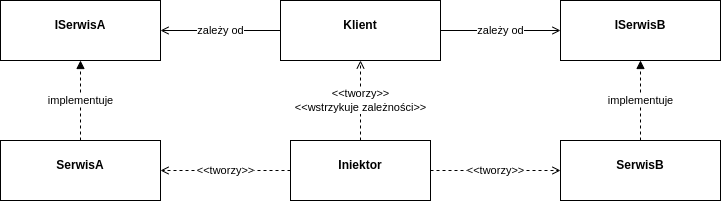
\includegraphics[width=\textwidth]{img/chapter5/dependency_injection.png}
    \caption{Wizualizacja wzorca projektowego zastrzyków zależności w postaci diagramu klas}
    \label{fig:dependency_injection}
\end{figure}

Same zastrzyki są procesem tworzenia i przekazywania obiektów serwisów, do zależnych od nich klientów, przy pomocy obiektu Iniektora. Na rys. \ref{fig:dependency_injection} przedstawiono prostą wizualizację zastosowania wzorca. Zadaniem takiego rozwiązania jest zmniejszenie do minimum, ilości twardych powiązań klas w projektach programów. Czyni je to bardziej skalowalnymi, łatwiejszymi w testowaniu oraz dokumentowaniu i obiektywnie lepszymi programistyczne rozwiązaniami (np. zachowanie zasady pojedynczej odpowiedzialności komponentów).

Zastrzyk zależności może nastąpić na trzy różne sposoby. Najpopularniejszą z metod, jest przekazywanie tworzonego obiektu przez interfejs, będący argumentem konstruktora obiektu klienta. Pozostałe dwie to: przekazanie obiektu przy pomocy metody dostępowej pola C\# lub przez argument dowolnej innej metody klasy. Najwięcej zalet, posiada metoda wykorzystująca konstruktor, która pozwala uniknąć odwołań do referencji serwisów wskazujących na adres zerowy, ustawiając ich adres przy tworzeniu obiektu klienta.

Kolejnym ważnym elementem, jest kontener odwróconej kontroli (IoC), umożliwiający automatyzację procesu wstrzykiwania zależności w aplikacjach. W przypadku platformy ASP.NET Core, podstawowy kontener IoC jest zawarty w jej kodzie, umożliwiając łatwe rozpoczęcie pracy z tym wzorcem. Przykłady jego użycia można znaleźć w metodzie ConfigureServices() klasy Startup (patrz listing \ref{lst:startup_server}). Obiekt implementujący interfejs IServiceCollection, przekazywany jest do niej jako argument i umożliwia ręczną konfigurację zależności, wykorzystywanych przez automatyczny iniektor platformy.

\begin{lstlisting}[language=CSharp, caption=Fragment ciała metody Startup.ConfigureServices() poświęcony konfiguracji przekierowania do strony w wersji HTTPS, label=lst:startup_configureServices_basics]
services.AddHttpsRedirection(options => {
  options.RedirectStatusCode = (int)HttpStatusCode.PermanentRedirect;
  options.HttpsPort = _env.IsDevelopment() ? 5001 : 443;
});
\end{lstlisting}

Wiele ze wstrzykiwanych w ten sposób serwisów, konfiguruje się wykorzystując metody rozszerzające kolekcję serwisów, zdefiniowane w poszczególnych bibliotekach. Przykładowo, fragment z listingu \ref{lst:startup_configureServices_basics} wywołuje metodę rejestrującą serwis obsługujący przekierowanie klienta na stronę w wersji HTTPS. Jednakże, chcąc zarejestrować serwisy zdefiniowane przez użytkownika, można posłużyć się trzema dostępnymi metodami generycznymi, określającymi cykl życia danego serwisu:

\begin{itemize}
    \item AddSingleton() - obiekt serwisu zarejestrowanego przy pomocy metody singleton, zostaje utworzony tylko raz, przy pierwszym wstrzyknięciu i jest współdzielony między wszystkimi zależnymi od niego klientami, aż do końca życia aplikacji. Wykorzystanie wzorca projektowego singleton w ten sposób, zapewnia również implementację, potencjalnie lepiej przystosowaną do wielowątkowości.
    \item AddScoped() - rejestrując serwisy ograniczone zakresem żądania, zapewniamy, że tworzone obiekty zostają użyte tylko w ramach konkretnego żądania HTTP. Obiekty są tworzone na początku konkretnego żądania HTTP i są współdzielone między wszystkimi klientami, obsługującymi to żądanie.
    \item AddTransient() - obiekty serwisów przemijających, są tworzone ekskluzywnie dla każdego klienta, gdy są potrzebne. Nigdy nie są współdzielone między różnymi klientami.
\end{itemize}

Fragmenty kodu rejestrującego serwisy, powiązane z poszczególnymi zadaniami, zostały przytoczone w odpowiednich sekcjach dalszej części pracy. 

%%%%%%%%%%%%%%%%%%%%%%%%%%%%%%%%%%%%%%%%%%%%%%%%%%%%%%%%%%%%%%%%%%%%%%%%%%%%%%%%
\section{Kontekst bazy danych i migracje Entity Framework Core}
%%%%%%%%%%%%%%%%%%%%%%%%%%%%%%%%%%%%%%%%%%%%%%%%%%%%%%%%%%%%%%%%%%%%%%%%%%%%%%%%

Kolejnym tematem jest sposób połączenia aplikacji z bazą danych. Aplikacja wykorzystuje ORM EF Core dla, którego najważniejszą klasą jest kontekst bazy danych.

\begin{lstlisting}[language=CSharp, caption=Klasa kontekstu bazy danych, label=lst:appDbContext]
public class AppDbContext : IdentityUserContext<User, int> {
  private readonly int _userId;

  public AppDbContext() { }

  public AppDbContext(DbContextOptions<AppDbContext> options) : base(options) { }

  public AppDbContext(DbContextOptions<AppDbContext> options, 
      IUserClaimsService<int> userClaims) : base(options) {
    _userId = userClaims.UserId;
  }

  public virtual DbSet<Action> Actions { get; set; }
  public virtual DbSet<ActionEquipment> ActionEquipment { get; set; }
  public virtual DbSet<ActionMember> ActionMembers { get; set; }
  public virtual DbSet<Equipment> Equipment { get; set; }
  public virtual DbSet<Member> Members { get; set; }
  public override DbSet<User> Users { get; set; }

  protected override void OnModelCreating(ModelBuilder builder) {
    base.OnModelCreating(builder);
    ...
  }

  public override async Task<int> SaveChangesAsync(CancellationToken cancellationToken = default) {
    ...
  }
}
\end{lstlisting}

Na listingu \ref{lst:appDbContext} ukazano najważniejszą część klasy kontekstu, w której publiczne pola o generycznych typach DbSet, reprezentują poszczególne tabele (relacje) zasobów w bazie danych. Oprócz konstruktorów, umożliwiających skonfigurowanie połączenia z bazą danych, kontekst posiada zasłoniętą metodę OnModelCreating(), której ciało umożliwia zastosowanie dodatkowej konfiguracji na relacji w bazie danych.

\begin{lstlisting}[language=CSharp, caption=Przykładowa klasa konfiguracyjna relacji w bazie danych wykorzystująca interfejs biegły Entity Framework Core, label=lst:member_config]
internal class MemberConfiguration : IEntityConfiguration {
  public void AddConfiguration(ModelBuilder builder) {
    builder.Entity<Member>(entity => {
      entity.HasKey(e => e.Id);
      entity.Property(e => e.Id)
        .IsRequired()
        .ValueGeneratedOnAdd();
      entity.Property(e => e.FirstName)
        .IsRequired()
        .HasMaxLength(24);
      entity.Property(e => e.LastName)
        .IsRequired()
        .HasMaxLength(24);
      entity.Property(e => e.Pesel)
        .HasColumnType("char(11)")
        .IsRequired()
        .HasMaxLength(11);
      entity.Property(e => e.UserId)
        .HasColumnName("OwnerId")
        .IsRequired();
      entity.HasOne(e => e.User)
        .WithMany(e => e.Members)
        .OnDelete(DeleteBehavior.NoAction);
      entity.HasMany(e => e.Actions)
        .WithOne(e => e.Member)
        .OnDelete(DeleteBehavior.Cascade);
    });
  }

  public void SeedData(ModelBuilder builder) {
    ...
  }
}
\end{lstlisting}

Konfigurację poszczególnych zasobów podzielono na klasy, zawierające dwie metody. Metoda AddConfiguration() służy wprowadzeniu ograniczeń dla atrybutów zasobu oraz określaniu jego relacji jeden-do-wielu, wiele-do-jednego oraz jeden-do-jednego. Druga metoda, SeedData() służy do utworzenia encji, automatycznie wpisanych do tabeli podczas tworzenia bazy.

Przykładowa konfiguracja, zasobu członka zespołu z listingu \ref{lst:member_config} określa typ kolumny Pesel jako char(11), czyniąc ją jednocześnie wartością wymaganą i ograniczając maksymalną długość jej wartości do 11 znaków. Na budowniczym encji, użyto metod definiujących jej relację wiele-do-jednego z właścicielem encji członka zespołu oraz relacji jeden-do-wielu z akcjami, w których wziął udział.

\begin{lstlisting}[language=CSharp, caption=Fragment metody AppDbContext.OnModelCreating() poświęcony klasom konfiguracyjnym encji, label=lst:onModelCreating_configs]
IEnumerable<IEntityConfiguration> entityConfigurations = new List<IEntityConfiguration> {
  new ActionConfiguration(),
  new ActionEquipmentConfiguration(),
  new ActionMemberConfiguration(),
  new EquipmentConfiguration(),
  new MemberConfiguration(),
  new UserConfiguration()
};
foreach (var entityConfiguration in entityConfigurations) {
  entityConfiguration.AddConfiguration(builder);
  entityConfiguration.SeedData(builder);
}
\end{lstlisting}

Konfiguracje można wykorzystać w metodzie OnModelCreating() kontekstu. Część z zastosowanych w nich opcji jest redundantne, względem adnotacji danych w klasie zasobu. Jednakże, niektóre ograniczenia są możliwe tylko dzięki biegłemu interfejsowi (Fluent API) EF Core. Przykładem takich ustawień, jest zastosowanie klucza złożonego (składającego się z więcej niż jednego atrybutu) oraz zastosowanie ochrony per-wiersz, opisanej w sekcji poświęconej użytkownikom systemu.

\begin{lstlisting}[language=CSharp, caption=Rejestracja kontekstu bazy danych jako serwis w metodzie Startup.ConfigureServices(), label=lst:config_appDbContext]
services.AddDbContext<AppDbContext>(options => {
  options.UseNpgsql(
      Configuration.GetConnectionString("PostgreSql"),
      builder => builder.EnableRetryOnFailure(5, TimeSpan.FromSeconds(10), null)
    )
    .EnableSensitiveDataLogging(false);
});
\end{lstlisting}

W celu zarejestrowania kontekstu bazy danych, jako serwisu do wstrzykiwania w zależnych od niego klientach, należy dodać fragment kodu widoczny na listingu \ref{lst:config_appDbContext} do ciała funkcji Startup.ConfigureServices(). 

\begin{lstlisting}[language=JavaScript, caption=Fragment pliku konfiguracyjnego appsettings.json zawierający łańcuch połączenia z bazą danych, label=lst:appsettings_conStr]
"ConnectionStrings": {
  "PostgreSql": "Host=ec2-18-202-156-92.eu-west-1.compute.amazonaws.com;Port=5432;Database=d92n4e7hua6lht;Username=lundqzkmrjkhry;Password=1e089e898b0ee3a9a3863e3be4921f37ed691a8a40dc2c02d876c382934d29c8"
 },
\end{lstlisting}

Wstrzyknięty na etapie budowania, serwis IConfiguration umożliwia uzyskanie łańcucha połączenia z bazą, przy pomocy dedykowanej metody serwisu konfiguracyjnego GetConnectionString().

Ostatnią częścią, klas odpowiedzialnych za interakcje z bazą danych, są migracje. Po zarejestrowaniu kontekstu bazy jako serwis, dostępne staje się narzędzie konsolowe dotnet-ef. Umożliwia tworzenie migracji modelu oraz aktualizowanie struktury bazy danych.

\begin{lstlisting}[language=CSharp, caption=Przykładowa klasa migracji Entity Framework Core, label=lst:migration]
public partial class Members_Pesel_TypeFromVarcharToChar : Migration
{
    protected override void Up(MigrationBuilder migrationBuilder)
    {
        migrationBuilder.AlterColumn<string>(
            name: "Pesel",
            table: "Members",
            type: "char(11)",
            maxLength: 11,
            nullable: false,
            oldClrType: typeof(string),
            oldType: "varchar(11)",
            oldMaxLength: 11);
    }

    protected override void Down(MigrationBuilder migrationBuilder)
    {
        migrationBuilder.AlterColumn<string>(
            name: "Pesel",
            table: "Members",
            type: "varchar(11)",
            maxLength: 11,
            nullable: false,
            oldClrType: typeof(string),
            oldType: "char(11)",
            oldMaxLength: 11);
    }
}
\end{lstlisting}

Przykładowa klasa migracji (a właściwie jej czytelna dla ludzi część), utworzona na etapie optymalizacji zapytań do bazy danych, została pokazana na listingu \ref{lst:migration}. Tworząc ją, zamieniono typ kolumny atrybutu Pesel w tabeli członków zespołu, z varchar(11) na char(11). Pozwala to na oszczędność miejsca w bazie oraz zoptymalizowanie procesu wyboru krotek encji.

Metoda Up() migracji wskazuje, jakie zapytania powinny zostać wykonane przez ORM, aby zastosować zmiany, dokonane w kodzie modelu bazy (zasobów i kontekstu). Metoda Down() jest stosowana w przypadku cofania tych zmian. Jednakże, jak zostało opisane w sekcji rozdziału teoretycznego poświęconemu narzędziom ORM, zawsze należy upewnić się czy zastosowanie lub wycofanie danej migracji nie wiąże się z ryzykiem utraty danych.

%%%%%%%%%%%%%%%%%%%%%%%%%%%%%%%%%%%%%%%%%%%%%%%%%%%%%%%%%%%%%%%%%%%%%%%%%%%%%%%%
\section{Warstwy interfejsu REST}
%%%%%%%%%%%%%%%%%%%%%%%%%%%%%%%%%%%%%%%%%%%%%%%%%%%%%%%%%%%%%%%%%%%%%%%%%%%%%%%%

W tej sekcji opisano trzy rodzaje klas składających się na funkcjonalności interfejsu REST aplikacji serwerowej.

%%%%%%%%%%%%%%%%%%%%%%%%%%%%%%%%%%%%%%%%%%%%%%%%%%%%%%%%%%%%%%%%%%%%%%%%%%%%%%%%
\subsection{Repozytoria}
%%%%%%%%%%%%%%%%%%%%%%%%%%%%%%%%%%%%%%%%%%%%%%%%%%%%%%%%%%%%%%%%%%%%%%%%%%%%%%%%

\begin{lstlisting}[language=CSharp, caption=Generyczna klasa podstawowego repozytorium zasobów, label=lst:repository]
public class Repository<T> : IRepository<T> where T : class {
  private readonly AppDbContext _context;

  public Repository(AppDbContext context) {
    _context = context;
  }

  public void Create(T entity) {
    _context.Add(entity);
  }

  public void Update(T entity) {
    _context.Update(entity);
  }

  public void Delete(T entity) {
    _context.Remove(entity);
  }

  public virtual IQueryable<T> ReadAll() {
    return _context.Set<T>();
  }

  public IQueryable<T> ReadAll(PaginationFilter pagination) {
    return ReadAll().Skip((pagination.PageIndex - 1) * pagination.PageSize)
      .Take(pagination.PageSize);
  }

  public async Task<int> SaveChangesAsync() {
    return await _context.SaveChangesAsync();
  }
}
\end{lstlisting}

Repozytoria są klasami najbliższymi do warstwy danych. Odpowiadają za tworzenie zapytań do bazy danych, wykorzystując tzw. biegłe metody biblioteki LINQ na polach wstrzykniętego obiektu kontekstu bazy. W ramach metod zdefiniowanych w repozytoriach, nie dochodzi do przesłania zapytań, do silnika bazy danych. Dzieje się to dopiero w klasach serwisów, określających, jaką strukturę danych należy utworzyć ze zwróconych rekordów.

\begin{lstlisting}[language=CSharp, caption=Generyczne klasy repozytoriów dla zasobów posiadających klucz główny lub klucz złożony z dwóch atrybutów, label=lst:repository_id]
public class HasIdRepository<T, TId>
  : Repository<T>, IHasIdRepository<T, TId>
  where T : class, IHasId<TId>
  where TId : IEquatable<TId>, IComparable<TId> {
  public HasIdRepository(AppDbContext context) : base(context) {
  }

  public virtual IQueryable<T> ReadById(TId id) {
    return ReadAll().Where(e => e.Id.Equals(id));
  }
}

public class HasIdRepository<T, TId, TId2>
  : HasIdRepository<T, TId>, IHasIdRepository<T, TId, TId2>
  where T : class, IHasId<TId, TId2>
  where TId : IEquatable<TId>, IComparable<TId>
  where TId2 : IEquatable<TId2>, IComparable<TId2> {
  public HasIdRepository(AppDbContext context) : base(context) {
  }

  public IQueryable<T> ReadById(TId id, PaginationFilter pagination) {
    return ReadById(id).Skip((pagination.PageIndex - 1) * pagination.PageSize)
      .Take(pagination.PageSize);
  }

  public IQueryable<T> ReadById(TId id, TId2 id2) {
    return ReadById(id).Where(e => e.Id2.Equals(id2));
  }
}
\end{lstlisting}

Aby zarejestrować klasy repozytoriów w kontenerze IoC aplikacji, dodano fragment kodu z listingu \ref{lst:config_repositories}, w metodzie Startup.ConfigureServices(). Obiekty repozytoriów zostają wstrzyknięte do serwisów, w zakresie pojedynczego żądania REST.

\begin{lstlisting}[language=CSharp, caption={Fragment metody Startup.ConfigureServices(), rejestrujący klasy repozytoriów zasobów, w kontenerze IoC}, label=lst:config_repositories]
services.AddScoped<IHasIdRepository<OspM.Action, int>, HasIdRepository<OspM.Action, int>>();
services.AddScoped<IHasIdRepository<OspM.ActionEquipment, int, int>, ActionEquipmentRepository>();
services.AddScoped<IHasIdRepository<OspM.ActionMember, int, int>, ActionMembersRepository>();
services.AddScoped<IHasIdRepository<OspM.Equipment, int>, HasIdRepository<OspM.Equipment, int>>();
services.AddScoped<IHasIdRepository<OspM.Member, int>, HasIdRepository<OspM.Member, int>>();
\end{lstlisting}

%%%%%%%%%%%%%%%%%%%%%%%%%%%%%%%%%%%%%%%%%%%%%%%%%%%%%%%%%%%%%%%%%%%%%%%%%%%%%%%%
\subsection{Serwisy}
%%%%%%%%%%%%%%%%%%%%%%%%%%%%%%%%%%%%%%%%%%%%%%%%%%%%%%%%%%%%%%%%%%%%%%%%%%%%%%%%

Serwisy stanowią miejsce największej ilości procesów, zachodzących w warstwie logiki aplikacji. Niektóre z nich, służą jedynie wykonaniu zapytań do bazy danych za pośrednictwem repozytoriów oraz sprawdzeniu ich powodzenia. Inne, odpowiadają za operacje takie jak: wysyłanie e-maili czy uwierzytelnianie użytkowników w systemie.

\begin{lstlisting}[language=CSharp, caption=Fragment generycznej klasy serwisu operującego na encjach zasobów, label=lst:service]
public class Service<T> : IService<T> where T : class {
  private readonly IRepository<T> _repo;

  public Service(IRepository<T> repo) {
    _repo = repo;
  }

  public async Task Create(T entity) {
    _repo.Create(entity);
    await CommitDbTransaction(DbTransactionType.Create);
  }

  public async Task Update(T entity) {
    _repo.Update(entity);
    await CommitDbTransaction(DbTransactionType.Update);
  }

  ...

  public async Task CommitDbTransaction(int rows, DbTransactionType type) {
    if (await _repo.SaveChangesAsync() < 0) {
      throw new DbTransactionException<T>(type, rows);
    }
  }

  public async Task CommitDbTransaction(DbTransactionType type) {
    await CommitDbTransaction(1, type);
  }

  public async Task CommitDbTransaction() {
    await CommitDbTransaction(DbTransactionType.None);
  }
}
\end{lstlisting}

Serwis przedstawiony na listingu \ref{lst:service}, stanowi podstawę do wykonania operacji, na zasobach należących do użytkownika. W przypadku niepowodzenia, rzucany jest odpowiedni wyjątek, wymagający obsłużenia w kolejnej, bardziej abstrakcyjnej warstwie projektu. Przykładowo, w metodzie ReadById() serwisu przedstawionego na kolejnym listingu \ref{lst:service_id}, może zostać rzucony wyjątek, informujący o tym, że nie odnaleziono encji o wskazanym kluczu głównym.

\begin{lstlisting}[language=CSharp, caption=Generyczna klasa serwisu operującego na encjach zasobów posiadających klucz główny, label=lst:service_id]
public class HasIdService<T, TId> : Service<T>, IHasIdService<T, TId>
  where T : class, IHasId<TId>
  where TId : IEquatable<TId>, IComparable<TId>, IConvertible {
  private readonly IHasIdRepository<T, TId> _repo;

  public HasIdService(IHasIdRepository<T, TId> repo) : base(repo) {
    _repo = repo;
  }

  public virtual async Task<T> ReadById(TId id) {
    var entity = await _repo.ReadById(id).FirstOrDefaultAsync();
    if (entity == default(T)) {
      throw new NotFoundException<T, TId>(id);
    }
    return entity;
  }
}
\end{lstlisting}

Podobnie jak w przypadku klas repozytoriów, klasy serwisów zostają zarejestrowane w kontenerze IoC aplikacji, w metodzie Startup.ConfigureServices(). Fragment kodu na listingu \ref{lst:config_services} pokazuje dodatkowo, proces rejestracji maperów klas zasobów, wstrzykiwanych razem z serwisami w warstwie kontrolerów aplikacji.

\begin{lstlisting}[language=CSharp, caption={Fragment metody Startup.ConfigureServices(), rejestrujący przykładowe klasy serwisów oraz maperów klas zasobów, w kontenerze IoC}, label=lst:config_services]
services.AddScoped<IHasIdService<OspM.Equipment, int>, HasIdService<OspM.Equipment, int>>();
services.AddScoped<IHasIdService<OspM.Member, int>, HasIdService<OspM.Member, int>>();
...
services.AddScoped<IDtoMapper<OspM.Member, MemberCreateDto, MemberReadDto, MemberUpdateDto>, MemberDtoMapper>();
services.AddScoped<IUserDtoMapper, UserDtoMapper>();
\end{lstlisting}

%%%%%%%%%%%%%%%%%%%%%%%%%%%%%%%%%%%%%%%%%%%%%%%%%%%%%%%%%%%%%%%%%%%%%%%%%%%%%%%%
\subsection{Kontrolery}
%%%%%%%%%%%%%%%%%%%%%%%%%%%%%%%%%%%%%%%%%%%%%%%%%%%%%%%%%%%%%%%%%%%%%%%%%%%%%%%%

Najbardziej abstrakcyjnym elementem aplikacji serwerowej są kontrolery, mogące być utożsamiane z reprezentacją interfejsu REST, udostępnianą klientom przez aplikację serwerową. W ciałach ich klas, zdefiniowane zostają punkty końcowe, w postaci metod obsługujących żądania przychodzące.

\begin{lstlisting}[language=CSharp, caption={Generyczna klasa kontrolera, bazująca na klasach zasobu oraz klasach jego reprezentacji}, label=lst:controller]
[Route("api/[controller]")]
public class Controller<T, TCreateDto, TReadDto, TUpdateDto> : ControllerBase
  where T : class
  where TCreateDto : class
  where TReadDto : class
  where TUpdateDto : class {
  protected readonly IDtoMapper<T, TCreateDto, TReadDto, TUpdateDto> _mapper;

  protected readonly IService<T> _service;

  public Controller(
    IService<T> service,
    IDtoMapper<T, TCreateDto, TReadDto, TUpdateDto> mapper) {
    _service = service;
    _mapper = mapper;
  }
  ...
}
\end{lstlisting}

Klasa generycznego kontrolera, którego podstawowe pola przedstawiono na listingu \ref{lst:controller}, wykorzystuje wstrzykiwane w niego obiekty serwisu oraz mapera zasobu, w celu wykonania operacji zleconej przez przychodzące żądanie. 

Dzięki adnotacji Route nad definicją klasy, wszystkie klasy konkretne (concrete), które dziedziczą po klasie kontrolera generycznego lub jego pochodnych, będą obsługiwały żądania, dla których ścieżka do zasobu, zaczyna się od frazy "/api/[controller]". Adnotacja przeprowadza wycięcie łańcucha "Controller", z nazwy typu konkretnej klasy kontrolera i wstawia otrzymany łańcuch znaków w miejscu znacznika "[controller]".

\begin{lstlisting}[language=CSharp, caption={Publiczne metody klasy generycznej kontrolera}, label=lst:controller_methods]
[HttpGet]
public virtual async Task<ActionResult<IEnumerable<TReadDto>>> ReadAll() {
  ...
}

[HttpGet("count")]
public virtual async Task<ActionResult<int>> ReadCount() {
  ...
}

[HttpPost]
public virtual async Task<ActionResult<TReadDto>> Create(TCreateDto createDto) {
  ...
}
\end{lstlisting}

Metody kontrolerów opatrzone są adnotacjami, wskazującymi jakie metody HTTP powinny obsługiwać, dla określonej ścieżki zasobu. Na listingu \ref{lst:controller_methods}, przedstawiono następujące metody kontrolera:

\begin{itemize}
    \item ReadAll(), odpowiadającą na żądania "GET /api/[controller]", zwracającą w ciele odpowiedzi HTTP, tablicę obiektów reprezentacji odczytu w formacie JSON, wszystkich encji danego zasobu, do których użytkownik uzyskał autoryzację.
    \item ReadCount(), odpowiadającą na żądania "GET /api/[controller]/count", zwracającą pojedynczą liczbę całkowitą, w ciele odpowiedzi HTTP, wskazującą ilość encji danego zasobu, do których użytkownik uzyskał autoryzację.
    \item Create(), odpowiadającą na żądania "POST /api/[controller]", zwracającą w ciele odpowiedzi, reprezentację odczytu, utworzonej encji zasobu, w formacie JSON. Jako argument, przyjmuje z ciała żądania HTTP, reprezentację tworzenia zasobu, parsując notację JSON na obiekt języka C\#.
\end{itemize}

\begin{lstlisting}[language=CSharp, caption={Przykładowe ciało metody obsługującej żądanie oraz metody pomocnicze klasy generycznej kontrolera}, label=lst:controller_example_method]
[HttpPost]
public virtual async Task<ActionResult<TReadDto>> Create(TCreateDto createDto) {
  try {
    var entity = await CreateEntity(createDto);
    var readDto = _mapper.MapRead(entity);
    return CreatedAtAction(null, readDto);
  }
  catch (UnauthorizedException) {
    return Unauthorized();
  }
  catch (ValidationProblemException) {
    return ValidationProblem();
  }
  catch (DbTransactionException) {
    return StatusCode(StatusCodes.Status500InternalServerError);
  }
  catch {
    return StatusCode(StatusCodes.Status500InternalServerError);
  }
}

...

protected async Task<T> CreateEntity(T entity) {
  await _service.Create(entity);
  return entity;
}

protected virtual async Task<T> CreateEntity(TCreateDto createDto) {
  if (TryValidateModel(createDto) == false) {
    throw new ValidationProblemException();
  }
  var entity = _mapper.MapCreate(createDto);
  return await CreateEntity(entity);
}

protected virtual ActionResult<TReadDto> ReadEntity(T entity) {
  var readDto = _mapper.MapRead(entity);
  return Ok(readDto);
}
\end{lstlisting}

Ciała metody kontrolerów zawierają bloki try...catch, zapewniające obsługę wyjątków, rzuconych we wszystkich warstwach aplikacji. W sytuacji złapania poszczególnych wyjątków, metoda zwraca obiekt odpowiedniej klasy rezultatu, reprezentujący status odpowiedzi HTTP, inny niż status sukcesu. W celu uniknięcia powtórzeń w kodzie metod i kontrolerów pochodnych, zdefiniowane zostały chronione metody pomocnicze, wywołujące metody serwisu oraz maperów wstrzykniętych do kontrolera.

W przykładowej metodzie Create() ukazanej na listingu \ref{lst:controller_example_method}, waliduje się reprezentację zasobu przesłaną w żądaniu, aby następnie zmapować ją na obiekt encji zasobu przy pomocy wstrzykniętego mapera. Poprzez wywołanie dedykowanej metody serwisu, encja zostaje wpisana do tabeli w bazie danych. Po pomyślnym procesie zwrócony zostaje obiekt rezultatu, reprezentujący status "204 Created". Dodatkowo, ciało odpowiedzi zostaje uzupełnione reprezentacją odczytu utworzonej encji zasobu. 

\begin{lstlisting}[language=CSharp, caption={Generyczna klasa kontrolera zasobów posiadających klucz główny}, label=lst:hasIdController]
public class HasIdController<T, TCreateDto, TReadDto, TUpdateDto, TId>
  : Controller<T, TCreateDto, TReadDto, TUpdateDto>
  where T : class, IHasId<TId>
  where TCreateDto : class
  where TReadDto : class
  where TUpdateDto : class
  where TId : IEquatable<TId>, IComparable<TId> {
  protected new readonly IHasIdService<T, TId> _service;

  public HasIdController(
    IHasIdService<T, TId> service,
    IDtoMapper<T, TCreateDto, TReadDto, TUpdateDto> mapper)
    : base(service, mapper) {
    _service = service;
    
  ...
}
\end{lstlisting}

Podobnie jak w przypadku repozytoriów i serwisów, warstwa kontrolerów wykorzystuje dziedziczenie, w celu wykorzystania wcześniej zdefiniowanego kodu w bardziej wyspecjalizowanych klasach. Na listingu \ref{lst:hasIdController} ukazano fragment definicji kontrolera generycznego, operującego na zasobach posiadających klucz główny. 

Chronione enkapsulacją pole podstawowego serwisu IService, zostało w nim zasłonięte przez pole klasy IHasIdService. Klasa dziedziczy po IService podstawowe pola oraz rozbudowuje ją o metody związane z kluczem głównym zasobu. Dzięki zastosowanemu dziedziczeniu klas i interfejsów w projekcie, nowy serwis może zostać przekazany do klasy bazowej kontrolera, za pośrednictwem rodzica interfejsu, który implementuje.

\begin{lstlisting}[language=CSharp, caption={Przykładowe metody generycznej klasy kontrolera zasobów posiadających klucz główny}, label=lst:hasIdController_methods]
[HttpGet("{id}")]
public virtual async Task<ActionResult<TReadDto>> ReadById(TId id) {
  try {
    var entity = await _service.ReadById(id);
    return base.ReadEntity(entity);
  }
  catch (UnauthorizedException) {
    return Unauthorized();
  }
  catch (NotFoundException) {
    return NotFound();
  }
  catch {
    return StatusCode(StatusCodes.Status500InternalServerError);
  }
}

[HttpPost]
public override async Task<ActionResult<TReadDto>> Create(TCreateDto createDto) {
  try {
    var entity = await base.CreateEntity(createDto);
    var readDto = _mapper.MapRead(entity);
    return CreatedAtAction(nameof(ReadById), new {id = entity.Id}, readDto);
  }
  catch (UnauthorizedException) {
    return Unauthorized();
  }
  catch (ValidationProblemException) {
    return ValidationProblem();
  }
  catch (DbTransactionException) {
    return StatusCode(StatusCodes.Status500InternalServerError);
  }
  catch {
    return StatusCode(StatusCodes.Status500InternalServerError);
  }
}
\end{lstlisting}

Listing \ref{lst:hasIdController_methods} przedstawia nową metodę ReadById() oraz nadpisaną metodę wirtualną Create(). Pierwsza wykorzystuje metodę rozszerzonego serwisu, w celu zwrócenia reprezentacji encji zasobu o konkretnym identyfikatorze. Żądanie "GET /api/[controller]/{id}" przeszukuje encje w tabeli po identyfikatorze, przesłanym jako część URI w miejscu znacznika {id}. 

Nadpisana metoda Create() zwraca bardziej kompletny obiekt rezultatu. Ciało odpowiedzi HTTP, emitowanej za jego pośrednictwem, zostaje uzupełnione o unikatowy identyfikator URI utworzonego zasobu, względem swojego poprzednika. Jest to jedna z polecanych praktyk, stosowanych w żądaniach REST, tworzących nowe zasoby.

\begin{lstlisting}[language=CSharp, caption={Generyczna klasa kontrolera autoryzowanego}, label=lst:authorizedController]
[Authorize(AuthenticationSchemes = JwtBearerDefaults.AuthenticationScheme)]
public class AuthorizedController<T, TCreateDto, TReadDto, TUpdateDto, TId>
  : HasIdController<T, TCreateDto, TReadDto, TUpdateDto, TId>
  where T : class, IHasId<TId>
  where TCreateDto : class
  where TReadDto : class
  where TUpdateDto : class
  where TId : IEquatable<TId>, IComparable<TId> {
  public AuthorizedController(
    IHasIdService<T, TId> service,
    IDtoMapper<T, TCreateDto, TReadDto, TUpdateDto> mapper)
    : base(service, mapper) {
  }
}
\end{lstlisting}

W celu łatwego zastosowania autoryzacji w aplikacji, zdefiniowano klasy generyczne kontrolerów autoryzowanych, dziedziczące po odpowiadających im kontrolerach generycznych. Adnotacja Authorize, użyta na listingu \ref{lst:authorizedController}, zapewnia autoryzacje dostępu klientów HTTP, do wszystkich zasobów udostępnianych przez metody tego kontrolera. Więcej informacji o konfiguracji schematu autoryzacji w aplikacji, znajduje się w osobnej, poświęconej temu sekcji.

\begin{lstlisting}[language=CSharp, caption={Przykładowa klasa konkretna kontrolera, udostępniająca zasoby REST}, label=lst:membersController]
[ApiController]
public class MembersController
  : AuthorizedController<Member, MemberCreateDto, MemberReadDto, MemberUpdateDto, int> {
  public MembersController(
    IHasIdService<Member, int> service,
    IDtoMapper<Member, MemberCreateDto, MemberReadDto, MemberUpdateDto> mapper)
    : base(service, mapper) {
  }
}
\end{lstlisting}

W odróżnieniu od klas repozytoriów i serwisów zasobów, klasy kontrolerów rejestruje się umieszczając nad definicją ich klasy adnotacje ApiController. Dzięki temu oznaczeniu, proces budowania aplikacji zinterpretuje ich metody, jako punkty końcowe interfesju REST.

\begin{lstlisting}[language=CSharp, caption={Przykładowa klasa konkretna, której odebrano funkcjonalności kontrolera}, label=lst:actionMembersController]
[NonController]
public class ActionMembersController
  : AuthorizedController<ActionMember, ActionMemberCreateDto, ActionMemberReadDto, ActionMemberUpdateDto, int, int> {
  public ActionMembersController(
    IHasIdService<ActionMember, int, int> service,
    IDtoMapper<ActionMember, ActionMemberCreateDto, ActionMemberReadDto, ActionMemberUpdateDto> mapper)
    : base(service, mapper) {
  }
}
\end{lstlisting}

\begin{lstlisting}[language=CSharp, caption={Fragment kontrolera akcji, wykorzystujący wstrzyknięcie kontrolera członków biorących udział w akcji}, label=lst:actionsController]
private readonly ActionMembersController _actionMembers;

public ActionsController(
  IHasIdService<Action, int> service,
  IDtoMapper<Action, ActionCreateDto, ActionReadDto, ActionUpdateDto> mapper,
  ActionEquipmentController actionEquipment,
  ActionMembersController actionMembers)
  : base(service, mapper) {
  _actionEquipment = actionEquipment;
  _actionMembers = actionMembers;
}

...

[HttpGet("{id}/members")]
public async Task<ActionResult<IEnumerable<ActionMemberReadDto>>> ReadMembers(int id) {
  return await _actionMembers.ReadById(id);
}

[HttpGet("{id}/members/count")]
public async Task<ActionResult<int>> ReadMembersCount(int id) {
  return await _actionMembers.ReadCount(id);
}

[HttpGet("{id}/members/{id2}")]
public async Task<ActionResult<ActionMemberReadDto>> ReadMember(int id, int id2) {
  return await _actionMembers.ReadById(id, id2);
}
\end{lstlisting}

Chcąc skorzystać z klasy kontrolera jak z obiektu wstrzykiwanego przez zależność do obiektu klienta, należy zastosować nad jego definicją adnotacje NonController. Pokazano to w przypadku kontrolera członków biorących udział w akcji na listingu \ref{lst:actionMembersController}. Jego obiekty wstrzyknięte zostały do kontrolera akcji, w celu ujednolicenia ścieżek URI, prowadzących do zasobów związanych z konkretnymi akcjami (listing \ref{lst:actionsController}).

\begin{lstlisting}[language=CSharp, caption={Rejestracja kontrolerów aplikacji w metodzie Startup.ConfigureServices()}, label=lst:config_controllers]
services.AddControllers()
  .AddNewtonsoftJson(s => {
    s.SerializerSettings.ContractResolver = new CamelCasePropertyNamesContractResolver();
  });
services.AddScoped<ActionEquipmentController>();
services.AddScoped<ActionMembersController>()
\end{lstlisting}

Kontrolery oznaczone przez adnotację ApiController, zostają zarejestrowane przy pomocy pojedynczej metody AddControllers(), użytej na obiekcie kolekcji serwisów, w metodzie Startup.ConfigureServices(). Pozostałe dwa, oznaczone adnotacją NonController, są rejestrowane przy pomocy standardowej metody kontenera (patrz listing \ref{lst:config_controllers}).

%%%%%%%%%%%%%%%%%%%%%%%%%%%%%%%%%%%%%%%%%%%%%%%%%%%%%%%%%%%%%%%%%%%%%%%%%%%%%%%%
\section{Aplikacja kliencka}
%%%%%%%%%%%%%%%%%%%%%%%%%%%%%%%%%%%%%%%%%%%%%%%%%%%%%%%%%%%%%%%%%%%%%%%%%%%%%%%%

Aplikacja kliencka utworzona w osobnym projekcie, dzięki platformie Blazor, jest świadczona za pośrednictwem punktów końcowych aplikacji serwerowej. Aby móc generować klasy na bazie komponentów Razor, dodano w metodzie Startup.ConfigrureServices(), linię kodu widoczną na listingu \ref{lst:config_razor}.

\begin{lstlisting}[language=CSharp, caption={Rejestracja serwisu, obsługującego komponenty Razor, w metodzie Startup.ConfigureServices()}, label=lst:config_razor]
services.AddRazorPages();
\end{lstlisting}

Następnie, skonfigurowano sposób przetwarzania żądań przesyłanych do aplikacji serwerowej, tak by zapewnić pierwszeństwo kontrolerom interfejsu REST. W drugiej kolejności przeszukiwane są treści, udostępnione za pośrednictwem odnośników na stronie aplikacji klienckiej.

\begin{lstlisting}[language=CSharp, caption={Konfiguracja punktów końcowych aplikacji serwerowej, w metodzie Startup.Configure()}, label=lst:config_endpoints]
app.UseRouting();
app.UseAuthorization();
app.UseBlazorFrameworkFiles();
app.UseStaticFiles();
app.UseEndpoints(endpoints => {
  endpoints.MapControllers();
  endpoints.MapFallbackToFile("{*path:nonfile}", "index.html");
});
\end{lstlisting}

Powyższy fragment kodu rozpoczyna się od uruchomienia usługi trasowania żądań HTTP, tak by mogły trafić do odpowiednich, abstrakcyjnych punktów końcowych stworzonych przez aplikację. Kolejna metoda uruchamia globalnie mechanizmy autoryzacji ASP.NET Core.

Następnie, konfigurowane są kolejno użycie plików załączonej przez referencje aplikacji Blazor oraz plików statycznych. Pliki statyczne takie jak: dokumenty HTML, arkusze CSS czy obrazy, występują w katalogu zwanym rdzeniem webowym aplikacji klienckiej, opisanym w jednej z poniższych podsekcji.

W ostatniej kolejności, zdefiniowane zostały punkty końcowe. Na początku zmapowane zostały punkty udostępnione przez kontrolery aplikacji serwerowej. Druga deklaracja, konfiguruje przeszukiwanie punktów końcowych, dostępnych jako ścieżki do stron-komponentów aplikacji klienckiej. Sama operacja analizuje treść pliku index.html, znajdującego się w rdzeniu webowym aplikacji.

%%%%%%%%%%%%%%%%%%%%%%%%%%%%%%%%%%%%%%%%%%%%%%%%%%%%%%%%%%%%%%%%%%%%%%%%%%%%%%%%
\subsection{Klasa konfiguracyjna}
%%%%%%%%%%%%%%%%%%%%%%%%%%%%%%%%%%%%%%%%%%%%%%%%%%%%%%%%%%%%%%%%%%%%%%%%%%%%%%%%

Projekt OpenOsp.Client posiada własną klasę Program, wykorzystywaną do konfiguracji serwisów, wstrzykiwanych do klas komponentów Razor, działających po stronie klienta. Proces konfiguracji obiektu klasy budowniczego projektu, odbywa się w metodzie Main(), która w przypadku samodzielnego projektu stanowi punkt startowy aplikacji Blazor.

\begin{lstlisting}[language=CSharp, caption={Konfiguracja głównego komponentu Razor w aplikacji klienckiej}, label=lst:blazor_root]
var builder = WebAssemblyHostBuilder.CreateDefault(args);
builder.RootComponents.Add<App>("#app");
\end{lstlisting}

Ciało metody, rozpoczyna się od zdefiniowania obiektu budowniczego programu WebAssembly. Następnie, zostaje określona klasa głównego komponentu Razor, stanowiącego punkt wyjścia dla funkcjonalności SPA aplikacji. Dynamicznie renderowana treść strony, jest wstawiana do treści dokumentu index.html, jako zawartość pojedynczego elementu, deklarujący identyfikator "app", przy pomocy atrybutu id.

\begin{lstlisting}[language=CSharp, caption={Rejestracja serwisu klienta HTTP w aplikacji klienckiej}, label=lst:blazor_http]
builder.Services.AddScoped(sp => new HttpClient {BaseAddress = new Uri(builder.HostEnvironment.BaseAddress)});
\end{lstlisting}

Jednym z najbardziej przydatnych narzędzi po stronie aplikacji klienckiej jest serwis klienta HTTP. Wstrzyknięty do komponentów aplikacji, umożliwia wysyłanie żądań oraz obsługę odpowiedzi HTTP, w każdym z nich.

\begin{lstlisting}[language=CSharp, caption={Rejestracja serwisu pamięci lokalnej w aplikacji klienckiej}, label=lst:blazor_localStorage]
builder.Services.AddBlazoredLocalStorage(config => {
  config.JsonSerializerOptions.DictionaryKeyPolicy = JsonNamingPolicy.CamelCase;
  config.JsonSerializerOptions.DefaultIgnoreCondition = JsonIgnoreCondition.WhenWritingNull;
  config.JsonSerializerOptions.IgnoreReadOnlyProperties = true;
  config.JsonSerializerOptions.PropertyNameCaseInsensitive = true;
  config.JsonSerializerOptions.PropertyNamingPolicy = JsonNamingPolicy.CamelCase;
  config.JsonSerializerOptions.ReadCommentHandling = JsonCommentHandling.Skip;
  config.JsonSerializerOptions.WriteIndented = false;
});
\end{lstlisting}

W ramach projektu skorzystano z zewnętrznej biblioteki, pozwalającej na eksploatację interfejsu pamięci lokalnej przeglądarki. Rejestrując odpowiedzialny za to zadanie interfejs, skonfigurowano również zasady serializacji danych w pamięci.

\begin{lstlisting}[language=CSharp, caption={Rejestracja serwisów związanych z autoryzacją i uwierzytelnieniem użytkownika, w aplikacji klienckiej}, label=lst:blazor_auth]
builder.Services.AddScoped<IAuthenticationService, AuthenticationService>();
builder.Services.AddAuthorizationCore();
builder.Services.AddScoped<AuthenticationStateProvider, AuthStateProvider>();
\end{lstlisting}

Aplikacja kliencka, podobnie jak serwerowa, wykorzystuje mechanizm autoryzacji, jednakże w celu zabezpieczenia wybranych widoków, przed nieuwierzytelnionymi użytkownikami. U podstaw działania uwierzytelniania i autoryzacji użytkownika w systemie, funkcjonują dwa dodatkowe serwisy, służące kolejno przeprowadzeniu procesu uwierzytelnienia oraz dostarczania informacji o stanie tokenów autoryzacyjnych w pamięci przeglądarki. Szczegóły ich implementacji zostały opisane w przeznaczonej ku temu sekcji.

\begin{lstlisting}[language=CSharp, caption={Wywołanie metody budującej i uruchamiającej aplikację kliencką}, label=lst:blazor_run]
await builder.Build().RunAsync();
\end{lstlisting}
 
Procesem zamykającym treść metody Main() jest wywołanie metod odpowiedzialnych za budowanie i uruchomienie aplikacji Blazor. Od tego momentu kontrola nad życiem aplikacji klienckiej, zostaje przekazana do aplikacji serwerowej.

%%%%%%%%%%%%%%%%%%%%%%%%%%%%%%%%%%%%%%%%%%%%%%%%%%%%%%%%%%%%%%%%%%%%%%%%%%%%%%%%
\subsection{Rdzeń webowy i środowisko uruchomieniowe .NET}
%%%%%%%%%%%%%%%%%%%%%%%%%%%%%%%%%%%%%%%%%%%%%%%%%%%%%%%%%%%%%%%%%%%%%%%%%%%%%%%%

\begin{figure}[!htbp] 
    \centering
    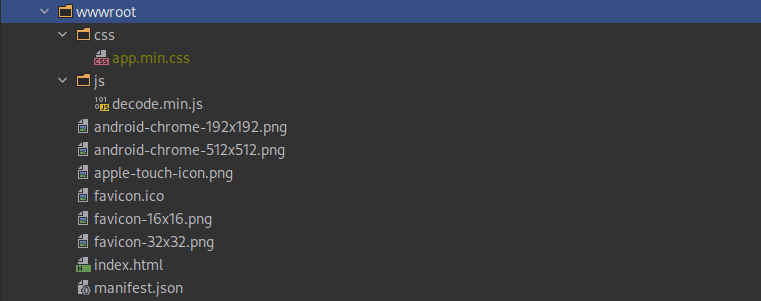
\includegraphics[width=\textwidth]{img/chapter5/wwwroot.png}
    \caption{Pliki w katalogu rdzenia webowego aplikacji klienckiej}
    \label{fig:wwwroot}
\end{figure}

Katalog wwwroot, ukazany na rys. \ref{fig:wwwroot}, znajduje się bezpośrednio w  katalogu głównym projektu aplikacji klienckiej. Nazywany jest rdzeniem webowym. Zawiera w sobie wszystkie serwowane przez system pliki statyczne.

\begin{lstlisting}[language=HTML, caption={Struktura dokumentu index.html w rdzeniu webowym aplikacji klienckiej}, label=lst:index_html]
<!DOCTYPE html>
<html class="w-full h-full">
<head>
  <meta charset="utf-8" />
  <meta content="width=device-width, initial-scale=1.0, maximum-scale=1.0, user-scalable=no" name="viewport" />
  <title>OpenOSP</title>
  <base href="/" />
  <link href="./css/app.min.css" rel="stylesheet" />
  <link href="./apple-touch-icon.png" rel="apple-touch-icon" sizes="180x180">
  <link href="./favicon-32x32.png" rel="icon" sizes="32x32" type="image/png">
  <link href="./favicon-16x16.png" rel="icon" sizes="16x16" type="image/png">
  <link href="./manifest.json" rel="manifest">
</head>
<body>
  ...
</body>
</html>
\end{lstlisting}

Dokument /wwwroot/index.html jest punktem wyjściowym aplikacji. Jego struktura, przedstawiona na listingu \ref{lst:index_html}, nie różni się niczym od struktury standardowego dokumentu, opisanego w sekcji rozdziału teoretycznego, poświęconej dokumentom HTML. W jego nagłówku, zdefiniowano metadane aplikacji, wypunktowane poniżej:

\begin{itemize}
    \item Aplikacja korzysta z systemu kodowania znaków UTF-8.
    \item Widok aplikacji wykorzystuje szerokość urządzenia, które ją wyświetla, jako szerokość strony i nie zezwala na jej skalowanie.
    \item Tytułem karty, w której otworzono aplikację, jest "OpenOSP".
    \item Dokument importuje arkusz stylów CSS z pliku /wwwroot/css/app.min.css, którego pochodzenie opisano w podsekcji poświęconej klasom Tailwind CSS.
    \item Zdefiniowane ikony są wyświetlane obok nazwy karty przeglądarki i dostępne w trzech różnych formatach. Użyte pliki graficzne są plikami statycznymi, występującymi w rdzeniu webowym aplikacji.
    \item Załączony plik manifest.json, dostarcza przeglądarkom kilka podstawowych informacji o aplikacji. Mogą okazać się one przydatne, w przypadku użycia na aplikacji mechanizmu PWA lub kontenera widoku webowego (webview container).
\end{itemize}

\begin{lstlisting}[language=HTML, caption={Treść ciała dokumentu index.html w rdzeniu webowym aplikacji klienckiej}, label=lst:index_body]
<div class="w-full h-full" id="app">
  <div class="w-full h-full flex justify-center items-center bg-base-300">
    <button class="btn btn-primary btn-outline btn-lg loading">Loading OpenOSP...</button>
  </div>
</div>
<script autostart="false" src="_framework/blazor.webassembly.js"></script>
\end{lstlisting}

Ciało dokumentu index.html, składa się z przedstawionego już wcześniej elementu o identyfikatorze "app" oraz załadowania skryptu JS, będącego częścią platformy Blazor. Początkowo, zawartość elementu app wypełniającego całe pole widoku w przeglądarce, zawiera treść informującą użytkownika o procesie ładowania aplikacji. Załączony skrypt \_framework/blazor.webassembly.js, działa w tle jako zadanie asynchroniczne, nie blokując wątku interfejsu użytkownika, wskazującego ekran ładowania. 

Skrypt pobiera potrzebne moduły WebAssembly, tworzące bardzo kompaktową implementację środowiska uruchomieniowego .NET (Mono) oraz skompilowaną do kodu pośredniego aplikację kliencką, razem z wykorzystywanymi przez nią modułami bibliotek ASP.NET Core. W praktyce, pozwala to na wykorzystanie komponentów Razor aplikacji, bezpośrednio w przeglądarce, wykorzystując webowe środowisko uruchomieniowe, jako mediator między technologiami webowymi, a technologiami .NET. 

Środowisko opiera się jedynie na standardach rekomendowanych przez W3C, dlatego nie powoduje problemów z kompatybilnością tworzonych rozwiązań. W przyszłości planuje się wprowadzenie kompilatora języka pośredniego platformy .NET, na natywny kod binarny WASM, przyspieszając proces pobierania i wykonania aplikacji w przeglądarce.

Po załadowaniu potrzebnych komponentów do pamięci przeglądarki, aplikacja Blazor uruchomiona po stronie klienta, podmienia zawartość elementu app na szablon HTML, renderowany przez komponent główny aplikacji. Został on wcześniej określony, przy pomocy odpowiedniej metody budowniczego, w metodzie Main() programu. Kolejna podsekcja opisuje, czym dokładnie są komponenty Razor i w jaki sposób wprowadzają mechanizmy aplikacji SPA po stronie klienta.

%%%%%%%%%%%%%%%%%%%%%%%%%%%%%%%%%%%%%%%%%%%%%%%%%%%%%%%%%%%%%%%%%%%%%%%%%%%%%%%%
\subsection{Komponenty Razor}
%%%%%%%%%%%%%%%%%%%%%%%%%%%%%%%%%%%%%%%%%%%%%%%%%%%%%%%%%%%%%%%%%%%%%%%%%%%%%%%%

Platforma Blazor, umożliwia tworzenie komponentów aplikacji na dwa sposoby: przy pomocy rozszerzonej notacji Razor i klas C\#. Projekt wykorzystuje pierwszą metodę, która oferuje bardziej naturalny sposób pracy z technologiami webowymi. 

W czasie budowania aplikacji, notacja zostaje przeanalizowana i przekształcona na zwykłe klasy komponentów, tak by mogło z nich skorzystać środowisko uruchomieniowe. Wykorzystanie klas bezpośrednio, jest pomocne w przypadkach zaawansowanych komponentów generycznych i funkcjonalności niedostępnych za pośrednictwem notacji Razor.

\begin{lstlisting}[language=HTML, caption={Przykładowy komponent Razor, opisujący główny układ strony}, label=lst:razor_body]
@inherits LayoutComponentBase

<div class="drawer w-auto min-h-screen text-base-content">
  <input id="navdrawer" type="checkbox" class="drawer-toggle" @bind="_isNavdrawer"/>
  <div class="drawer-content min-h-screen items-stretch">
    <div class="hero min-h-screen flex flex-col bg-firefighters">
      <div class="hero-overlay bg-opacity-70"/>
      <Header/>
      <main class="hero-content w-11/12 max-w-screen-md m-1 p-2">
        @Body
      </main>
    </div>
    <Footer/>
  </div>
  <div class="drawer-side">
    <label for="navdrawer" class="drawer-overlay"/>
    <Nav @bind-IsNavdrawer="_isNavdrawer" class="menu w-80 p-4 overflow-y-auto bg-base-300 bg-opacity-90"/>
  </div>
</div>

@code {

  private bool _isNavdrawer { get; set; }

}
\end{lstlisting}

Jako przykład komponentu, na listingu \ref{lst:razor_body} przedstawiono główny układ strony, wykorzystywany na każdej ze stron aplikacji. Rozpoczyna się od deklaracji dziedziczenia po komponencie bazowym LayoutComponentBase, przez co może zostać wykorzystany później do okalania stron w projekcie.

Kolejnym elementem jest schemat HTML, określający sposób wyświetlania komponentu na stronie. Elementy <Header>, <Footer> i <Nav> są innymi komponentami zdefiniowanymi w aplikacji, zostaną zarejestrowane w instancji aplikacji, jako obiekty swoich klas, a ich schemat zostanie wstawiony w miejsce ich znacznika. 

Znak "@" umożliwia zastosowanie języka C\# wewnątrz schematu, jeśli chcemy np. wstawić wartość pola klasy albo utworzyć blok pętli lub instrukcję warunkową. Użycie znacznika "@Body", powoduje wstawienie w jego miejsce fragmentu HTML, który został przekazany do komponentu jako zawartość, między jego znacznikiem początkowym i końcowym. 

Ostatnim elementem jest blok kodu "@code", umożliwiający łatwą definicję pól klasy komponentu, takich jak: wartości, referencje i metody. Przykładowo, zdefiniowano pole przetrzymujące wartość bool, określające czy nawigacyjny panel boczny strony jest wysunięty.

\begin{lstlisting}[language=CSharp, caption={Fragment bloku kodu komponentu Nav, poświęcony dwustronnemu wiązaniu danych}, label=lst:razor_twoWayBinding]
[Parameter]
public bool IsNavdrawer { get; set; }

[Parameter]
public EventCallback<bool> IsNavdrawerChanged { get; set; }

[Parameter(CaptureUnmatchedValues = true)]
public IReadOnlyDictionary<string, object> AdditionalAttributes { get; set; }

private async Task OnNavClick() {
  IsNavdrawer = false;
  await IsNavdrawerChanged.InvokeAsync(IsNavdrawer);
}
\end{lstlisting}

Stan komponentów nie jest składowany przy pomocy dedykowanego mechanizmu stanu, a jedynie wewnątrz ich obiektów (pamięć WASM). Dlatego, ważnym mechanizmem w aplikacji są dowiązania danych. Na listingu \ref{lst:razor_body}, komponent układu strony dzieli się z komponentem Nav, wartością pola \_isNavdrawer przy pomocy atrybutu "@bind-Navdrawer".

Jest to specjalny rodzaj notacji umożliwiający dowiązanie dwukierunkowe, w którym obiekt emitujący wartość pola, może zostać powiadomiony o zmianie tej wartości, za pośrednictwem mechanizmu zdarzeń (Event).

W rzeczywistości,  atrybut na listingu \ref{lst:razor_twoWayBinding}, przypisuje wartość dwóm parametrom komponentu Nav. Pierwszy to IsNavdrawer przetrzymujący wartość przekazanego pola, a drugi to IsNavdrawerChanged definiujący zdarzenie wywoływane, aby zaktualizować wartość przekazywanego pola w komponencie emitującym.

Przykładowo, przy kliknięciu na link w panelu bocznym, jest on chowany przy pomocy metody OnNavClick(). Najpierw podmieniana jest wartość IsNavdrawer, a następnie wywołuje się zdarzenie, przekazujące nową wartość komponentowi nadrzędnemu, będącego tzw. konsumentem zdarzenia.

Parametry komponentów, są publicznymi polami klasy, zdefiniowanymi w bloku kodu komponentu i oznaczone adnotacją Parameter. W prostszym przypadku mogą służyć przekazaniu wartości jednostronnie, pomijając prefiks "@bind-" atrybutu, w schemacie komponentu emitującego. Aby wykorzystać atrybuty nie przekazane do konkretnego pola parametru, należy zdefiniować pole kolekcji par klucz-wartość i oznaczyć je adnotacją Parameter, wraz z opcjonalnym argumentem flagi CaptureUnmatchedValues.

\begin{lstlisting}[language=CSharp, caption={Fragmenty komponentu tabeli członków zespołu wykorzystujące kaskadowe parametry}, label=lst:razor_cascadingParameters]
...
    <tbody>
    @foreach (var member in _members) {
      <CascadingValue Value=@member>
        <MemberRecord OnUpdateCallback="UpdateTable"/>
      </CascadingValue>
    }
    </tbody>
...

@code {

  [CascadingParameter(Name = "CheckedMembers")]
  private IDictionary<int, string> _checkedMembers { get; set; }

  private IEnumerable<MemberReadDto> _members { get; set; } = new List<MemberReadDto>();
  ...
}
\end{lstlisting}

\begin{lstlisting}[language=CSharp, caption={Kaskadowe parametry, komponentu rekordu tabeli członków zespołu}, label=lst:razor_memberRecord]
[CascadingParameter]
private MemberReadDto _readDto { get; set; }

[CascadingParameter(Name = "CheckedMembers")]
private IDictionary<int, string> _checkedMembers { get; set; }
\end{lstlisting}

Zwykłe atrybuty, nie są jedynym sposobem na jednostronne przekazanie wartości między komponentami. Za pomocą tzw. kaskadowych parametrów, można znacznie uprościć sytuacje przekazywania tej samej wartości przez wiele warstw komponentów. 

Jest to możliwe, dzięki znacznikowi <CascadingValue>, przyjmującego atrybut Value, określający wartość do przekazania w dół hierarchii komponentów. Opcjonalny atrybut Name, ustanawia identyfikator emitowanej wartości, pozwalając na rozwiązanie konfliktów między kaskadowymi parametrami tego samego typu.

Przykład wykorzystania kaskadowych parametrów został pokazany na listingu \ref{lst:razor_cascadingParameters}. Do obiektów komponentu rekordu tabeli, utworzonych w pętli foreach, kaskadowo przekazuje się obiekty reprezentacji odczytu członków zespołu, pozyskanych z bazy danych. Każdy rekord odbiera go przy pomocy pola \_readDto, oznaczonego przez adnotacje CascadingParameter, ukazanego na listingu \ref{lst:razor_memberRecord}.

W odróżnieniu od zwykłych parametrów, parametry kaskadowe mogą korzystać z pól niepublicznych. Parametry przekazywane między komponentami Razor, podlegają rozróżnieniu na typy referencyjne i przekazywane przez wartość. Domyślnie, wartości te wpisywane są do oznaczonych pól posiadających ten sam typ, co emitowana wartość. 

Komponenty tabeli i rekordu zawierają pole kaskadowego parametru, przekazywanego przez identyfikator "CheckedMembers". Pierwszy z nich wykorzystuje go w przypadku usuwania zaznaczonych wartości, drugi indykuje stan zaznaczenia w swoim schemacie, bazując na zawartości kolekcji.

\begin{lstlisting}[language=CSharp, caption={Fragmenty komponentu logowania użytkownika, wykorzystujące zastrzyki zależności i bloki warunkowe}, label=lst:razor_dependencyInjection]
@inject IAuthenticationService _authService
@inject NavigationManager _navManager

...
    <button type="submit" class="@($"btn btn-primary {(isWaitingForResult ? "loading" : string.Empty)}")" disabled="@isWaitingForResult">
      @if (isWaitingForResult is false) {
        <span>Log in</span>
      }
      else {
        <span>Logging in...</span>
      }
    </button>
...

@code {

  private UserLoginDto _dto = new();

  private bool isWaitingForResult = false;
  
  ...

  private async Task HandleLogin() {
    isWaitingForResult = true;
    showAuthenticationError = false;
    var result = await _authService.Login(_dto);
    if (result is not null) {
      _navManager.NavigateTo("/userpanel");
    }
    else {
      isWaitingForResult = false;
      authenticationError = "There was a problem logging in";
      showAuthenticationError = true;
    }
  }
}
\end{lstlisting}

Komponenty Razor mogą korzystać z zastrzyków zależności, deklarując zależność od wybranych serwisów przy pomocy znacznika "@inject". Wstrzyknięte w ten sposób serwisy są dostępne w całym bloku kodu komponentu, jak i jego schemacie, pod nazwą wskazaną w deklaracji zależności. W rzeczywistości, wstrzykiwanie zostaje przeprowadzone w konstruktorze wygenerowanej klasy komponentu.

Jednym z zarejestrowanych domyślnie serwisów, jest NavigationManager, wstrzykiwany przykładowo na listingu \ref{lst:razor_dependencyInjection}. Jego metody stanowią alternatywny, do nawigacyjnych linków HTML, sposób nawigacji po stronach aplikacji. Najczęściej są wykorzystywane do automatyzacji tego procesu, w metodach komponentów.

Listing zawiera przykłady wykorzystania bloków warunkowych w notacji Razor. Wyrażenia warunkowe można stosować nie tylko pomiędzy kolejnymi znacznikami HTML, ale również w ich atrybutach. Pozwala to na skrócenie schematu komponentu i uniknięcie powtórzeń.

Atrybut disabled zastosowany w elemencie przycisku, stanowi przykład rozbudowania funkcjonalności standardu HTML. W zwykłym dokumencie jest on wykorzystywany jako flaga, wskazująca na nieaktywność elementu w interfejsie użytkownika, bez względu na przypisaną mu wartość. Notacja Razor umożliwia dowiązania do niego wartości bool, z pomocą której można dynamicznie włączać i wyłączać tą flagę.

\begin{lstlisting}[language=CSharp, caption={Komponent Razor tworzący odnośniki do swojej zawartości, przy pomocy znaczników page}, label=lst:razor_home]
@page "/"
@page "/about"
@page "/contact"
@page "/verify/{verificationString}"

...

@code {

  [Parameter]
  public string VerificationString { get; set; }

  private bool showVerificationSuccess = false;

  protected override async Task OnInitializedAsync() {
    if (string.IsNullOrEmpty(VerificationString) is false) {
      var verificationResult = await _http.GetAsync($"api/users/verify?{VerificationString}");
      if (verificationResult.IsSuccessStatusCode) {
        showVerificationSuccess = true;
      }
    }
  }

  protected override async Task OnAfterRenderAsync(bool firstRender) {
    if (firstRender && showVerificationSuccess) {
      await Task.Delay(10000);
      showVerificationSuccess = false;
      StateHasChanged();
      NavManager.NavigateTo("/");
    }
  }

}
\end{lstlisting}

Niektóre komponenty, przy pomocy znacznika @page, deklarują ścieżki URI punktów końcowych, dla których ich schemat zostanie wyrenderowany na stronie aplikacji. Można zadeklarować więcej niż jedną, prowadzącą do treści ścieżkę. Podobnie jak w przypadku punktów końcowych aplikacji serwerowej, ścieżki mogą zawierać w sobie wartości parametrów, które zostaną przypisane do pól oznaczonych jako parametry w kodzie komponentu.

Strona główna aplikacji, przedstawiona na listingu \ref{lst:razor_home}, pełni jednocześnie funkcję strony weryfikującej e-mail zarejestrowanego użytkownika. Pobierając wartość łańcucha weryfikacyjnego, przesyła jego treść w zapytaniu żądania do kontrolera aplikacji serwerowej, wykorzystując metodę OnInitializedAsync() wywoływaną po inicjalizacji komponentu. Druga z metod OnAfterRenderAsync(), wywoływana jest po zakończeniu renderowania komponentu. Po upływie 10 sekund od pierwszego wyrenderowania komponentu na stronie, likwiduje informację o udanej weryfikacji e-maila i przekierowuje użytkownika do ścieżki "/".

Obie funkcje stanowią przykład metod wirtualnych, dziedziczonych po implikowanej klasie bazowej, wywoływanych automatycznie w danym momencie cyklu życia komponentu Razor. Nadpisując ciała tych metod, można określić dokładny moment wykonania wybranych procedur związanych z danym komponentem lub jego pochodnymi.

\begin{lstlisting}[language=CSharp, caption={Główny komponent Razor aplikacji klienckiej}, label=lst:razor_app]
@using OpenOsp.Client.Components.Main
<Router AppAssembly="@typeof(Program).Assembly" PreferExactMatches="true">
  <Found Context="routeData">
    <AuthorizeRouteView RouteData="@routeData" DefaultLayout="@typeof(Body)">
      ...
    </AuthorizeRouteView>
  </Found>
  <NotFound>
    <CascadingAuthenticationState>
      <LayoutView Layout="typeof(Body)">
        <OpenOsp.Client.Pages.NotFound/>
      </LayoutView>
    </CascadingAuthenticationState>
  </NotFound>
</Router
\end{lstlisting}

Schemat głównego komponentu aplikacji, widoczny na listingu \ref{lst:razor_app}, odpowiada za wewnętrzne trasowanie do komponentów-stron. Element Router wykorzystuje informacje o bibliotece klas aplikacji klienckiej, w celu sporządzenia listy ścieżek punktów końcowych, dla których wyrenderowana zostanie odpowiednia zawartość. 

Element Found obsługuje sytuację odnalezienia komponentu-strony, pod wskazaną ścieżką, wstawiając jego schemat w środku głównego układu strony, pokazanego na listingu \ref{lst:razor_body}. W przypadku nie odnalezienia komponentu-strony pod wskazaną ścieżką, wyświetlony zostanie dedykowany tej sytuacji komponent, określony w elemencie NotFound.

\begin{figure}[!htbp] 
    \centering
    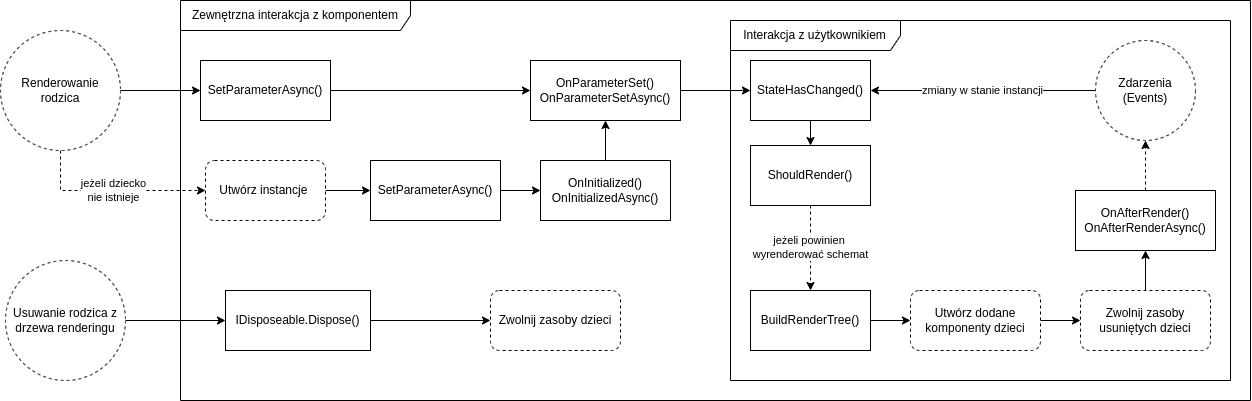
\includegraphics[width=\textwidth]{img/chapter5/razor.lifecycle.png}
    \caption{Cykl życia komponentów Razor}
    \label{fig:razor.lifecycle}
\end{figure}

Na rys. \ref{fig:razor.lifecycle} zaprezentowano cykl życia komponentów Razor. Struktura renderowanych przez aplikacje komponentów jest drzewem ich instancji, w którym korzeń stanowi unikatowa instancja komponentu App. Wewnątrz tego grafu, zmiany dokonane na instancji komponentu nadrzędnego (rodzica), implikują przymus ponownego wyrenderowania go i wszystkich podrzędnych mu instancji (dzieci). Jest to mechanizm optymalizacyjny aplikacji graficznych, tworzący podstawę działania aplikacji SPA. 

%%%%%%%%%%%%%%%%%%%%%%%%%%%%%%%%%%%%%%%%%%%%%%%%%%%%%%%%%%%%%%%%%%%%%%%%%%%%%%%%
\subsection{Generowanie arkusza CSS}
%%%%%%%%%%%%%%%%%%%%%%%%%%%%%%%%%%%%%%%%%%%%%%%%%%%%%%%%%%%%%%%%%%%%%%%%%%%%%%%%

W projekcie aplikacji zostały użyte narzędzia platformy NodeJS. W celu uproszczenia procesu stylizacji komponentów, zastosowano oparte o technologię JavaScript pakiety: TailwindCSS, Autoprefixer, CSSNano i PostCSS. 

\begin{lstlisting}[language=JavaScript, caption={Plik package.json w aplikacji klienckiej}, label=lst:package.json]
{
  ...
  "scripts": {
    "buildcss:dev": "cross-env TAILWIND_MODE=build postcss ./Styles/app.css -o ./wwwroot/css/app.min.css",
    "buildcss": "postcss ./Styles/app.css -o ./wwwroot/css/app.min.css"
  },
  ...
  "devDependencies": {
    "autoprefixer": "^10.3.4",
    "cross-env": "^7.0.3",
    "cssnano": "^5.0.8",
    "daisyui": "^1.14.0",
    "postcss": "^8.3.6",
    "postcss-cli": "^8.3.1",
    "tailwindcss": "^2.2.9",
    "tailwindcss-textshadow": "^2.1.3"
  }
}
\end{lstlisting}

Fragment pliku package.json, przedstawiony na listingu \ref{lst:package.json}, definiuje zbiór pakietów NodeJS potrzebnych podczas budowania aplikacji oraz dodatkowe skrypty pomocnicze. Narzędzie PostCSS, za pośrednictwem swoich rozszerzeń, wykorzystuje mechanizmy pozostałych trzech pakietów na wskazanym pliku wejściowym /Style/app.css. Umieszczony w rdzeniu webowym arkusz app.min.css, załączony w nagłówku dokumentu index.html, jest plikiem wynikowym tej operacji.

\begin{lstlisting}[language=CSS, caption={Plik /Styles/app.css w aplikacji klienckiej}, label=lst:app.css]
@tailwind base;
@tailwind components;
@tailwind utilities;
\end{lstlisting}

Plik /Styles/app.css zawiera kwerendy platformy TailwindCSS, wykorzystywane w procesie generacji arkusza CSS, używanego przez aplikację. W ich miejsce wstawiane są klasy CSS odpowiednich rodzajów, zdefiniowane przez pakiet.

\begin{lstlisting}[language=CSS, caption={Konfiguracja narzędzia TailwindCSS w pliku tailwind.config.js}, label=lst:tailwind]
module.exports = {
  mode: 'jit',
  purge: [
    './wwwroot/index.html',
    './**/*.razor',
  ],
  ...
}
\end{lstlisting}

Aby uniknąć generacji klas CSS niewykorzystywanych w projekcie, można zastosować tzw. generację w locie wraz z trybem czystki. Na listingu \ref{lst:tailwind}, deklarowane jest, że narzędzie powinno umieścić w pliku app.min.css tylko te klasy TaliwindCSS, które zostały wykorzystane przez dokument index.html lub którykolwiek z komponentów Razor, na wszystkich poziomach zagnieżdżenia projektu.

\begin{lstlisting}[language=HTML, caption={Fragment pliku OpenOsp.Client.csproj, automatyzujący generację arkusza CSS projektu}, label=lst:client_csproj]
<Target Name="NpmCheck" BeforeTargets="NpmInstall">
  <Exec Command="npm -v" ContinueOnError="true">
    <Output TaskParameter="ExitCode" PropertyName="ErrorCode" />
  </Exec>
  <Error Condition="'$(ErrorCode)' != '0'" Text="NPM not found. Please install Node.js and npm first." />
</Target>
<Target Name="NpmInstall" BeforeTargets="BuildCss" Inputs="./package.json" Outputs="$(NpmLastInstall)">
  <Exec Command="npm ci" />
  <Touch Files="$(NpmLastInstall)" AlwaysCreate="true" />
</Target>
<Target Name="BuildCss" BeforeTargets="Compile">
  <Exec Command="npm run buildcss" />
</Target>
\end{lstlisting}

Proces generacji klas i minimalizacji otrzymanego arkusza CSS, został zautomatyzowany przy pomocy konfiguracji w pliku OpenOsp.Client.csproj widocznej na listingu \ref{lst:client_csproj}. Notacja MSBuild sprawdza dostępność konsolowego menadżera pakietów npm i w razie potrzeby, instaluje nieobecne pliki pakietów NodeJS. Na końcu uruchamiany jest skrypt npm, zdefiniowany wcześniej w pliku package.json, generujący arkusz stylów aplikacji w rdzeniu webowym, jeszcze przed rozpoczęciem procesu kompilacji projektu.

%%%%%%%%%%%%%%%%%%%%%%%%%%%%%%%%%%%%%%%%%%%%%%%%%%%%%%%%%%%%%%%%%%%%%%%%%%%%%%%%
\subsection{Formularze i walidacja danych}
%%%%%%%%%%%%%%%%%%%%%%%%%%%%%%%%%%%%%%%%%%%%%%%%%%%%%%%%%%%%%%%%%%%%%%%%%%%%%%%%

Formularze danych to jedne z ważniejszych elementów interfejsu użytkownika. Twórcy platformy Blazor, zdefiniowali zbiór komponentów ułatwiających dowiązywanie danych, w polach formularza i wyświetlanie informacji zwrotnej o przebiegu ich walidacji.

\begin{lstlisting}[language=CSharp, caption={Przykład formularza danych w aplikacji klienckiej}, label=lst:editForm]
@inject HttpClient _http

...
  <EditForm Model="@_createDto" OnValidSubmit="HandleCreate" class="modal-box">
    ...
    <h1 class="mb-5 text-center text-2xl font-bold">Create a member</h1>
    <DataAnnotationsValidator/>
    <LabeledInputText @bind-Value="_createDto.FirstName"/>
    <LabeledInputText @bind-Value="_createDto.LastName"/>
    <LabeledInputText @bind-Value="_createDto.Pesel"/>
    <div class="modal-action">
      <button type="submit" class="@($"btn btn-primary {(isWaitingForResponse ? "loading" : string.Empty)}")" hidden="@isWaitingForResponse">Create</button>
      <label for="member-create-modal" class="btn" hidden="@isWaitingForResponse">Cancel</label>
    </div>
  </EditForm>
...

@code {
  
  ...
  private MemberCreateDto _createDto { get; set; } = new();
  ...

  private async Task HandleCreate() {
    showError = false;
    isWaitingForResponse = true;
    var result = await _http.PostAsJsonAsync("api/members", _createDto);
    isWaitingForResponse = false;
    ...
  }
  ...
}
\end{lstlisting}

Komponent EditForm jest wykorzystywany, do okalania formularzy, zamiast standardowego elementu <form>. Posiada osobne atrybuty, pozwalające określić metody obsługujące próby przesłania formularza dla danych poprawnych OnValidSubmit oraz dla niepoprawnych OnInvalidSubmit. Do przesyłania danych w formularzu, służy zwykły przycisk HTML typu submit.

Model danych, który podlega walidacji przez komponent formularza, jest przekazywany w atrybucie Model. Aby skorzystać z rezultatów walidacji poszczególnych pól formularza, przy pomocy ich adnotacji, należy umieścić dodatkowy komponent walidatora DataAnnotationsValidator, w zawartości formularza. 

\begin{lstlisting}[language=CSharp, caption={Rozszerzony komponent pola tekstowego formularza w aplikacji klienckiej}, label=lst:inputText]
@inherits InputText

<div class="form-control">
  @if (IsLabeled) {
    <label class="label">
      <LabelText For="@ValueExpression" class="label-text"/>
    </label>
  }
  <InputText @attributes="AdditionalAttributes"
             Value="@Value" ValueChanged="@ValueChanged" ValueExpression="@ValueExpression"
             class=@("input input-bordered " + CssClass.Replace(" valid", " input-success").Replace(" invalid", " input-error"))/>
  <label class="label">
    @SubLabel
    <div class="label-text-alt mx-2 text-error text-xs">
      <ValidationMessage For="@ValueExpression"/>
    </div>
  </label>
</div>
\end{lstlisting}

Komponent pola tekstowego, definiowanego przez platformę Razor, został rozszerzony w sposób pokazany na listingu \ref{lst:inputText}. Korzystając z biblioteki rozszerzeń formularzy, nad polem zostaje wyświetlona jego wizualna nazwa. Nazwy określić można w adnotacji Display, którą oznacza się pole klasy obiektu transferu danych (patrz listing \ref{lst:member_update_dto}).

% obraz udanej walidacji
\begin{figure}[!htbp]
\centering
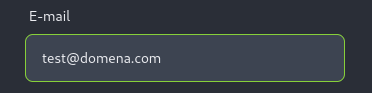
\includegraphics[width=\textwidth]{img/chapter5/form_valid.png}
\caption{Przykład udanej walidacji pola formularza}
\end{figure}

% obraz nieudanej walidacji
\begin{figure}[!htbp]
\centering
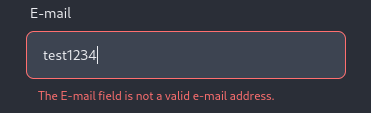
\includegraphics[width=\textwidth]{img/chapter5/form_invalid.png}
\caption{Przykład nieudanej walidacji pola formularza}
\end{figure}

Rezultat walidacji indykowany jest przy pomocy koloru obramowania pola tekstowego, ustawianego w dodatkowej logice stosowanej na klasach elementu. W przypadku niepowodzenia, wyświetlany jest komunikat o błędach walidacji.

%%%%%%%%%%%%%%%%%%%%%%%%%%%%%%%%%%%%%%%%%%%%%%%%%%%%%%%%%%%%%%%%%%%%%%%%%%%%%%%%
\section{Użytkownicy systemu}
%%%%%%%%%%%%%%%%%%%%%%%%%%%%%%%%%%%%%%%%%%%%%%%%%%%%%%%%%%%%%%%%%%%%%%%%%%%%%%%%

Interakcja z użytkownikami systemu, oparta jest o klasy biblioteki tożsamości ASP.NET Core, odpowiedzialnych m.in. za mechanizmy uwierzytelniania i autoryzacji w systemie. Aby składować informacje o użytkownikach i ich stanie, w bazie danych aplikacji, zaimportowano dedykowane temu rozszerzenie EF Core.

\begin{lstlisting}[language=CSharp, caption={Klasa zasobu użytkownika systemu}, label=lst:user]
public class User : IdentityUser<int> {
  ...
}
\end{lstlisting}

Na listingu \ref{lst:user}, klasa zasobu użytkownika rozszerza klasę generyczną IdentityUser, określając typ klucza głównego (identyfikatora) jako liczbę całkowitą. Dziedziczenie jest jednoznaczne z implementacją interfejsu, łączącego logicznie encje użytkowników i moduły biblioteki tożsamości.

\begin{lstlisting}[language=CSharp, caption={Konfiguracja serwisów związanych z użytkownikami w metodzie Startup.ConfigureServices()}, label=lst:config_users]
services.Configure<JwtSettings>(Configuration.GetSection("Jwt"));
services.Configure<EmailSettings>(Configuration.GetSection("Email"));
...
services.AddIdentityCore<OspM.User>(cfg => {
    cfg.User.RequireUniqueEmail = true;
    cfg.Password.RequireDigit = false;
    cfg.Password.RequireLowercase = false;
    cfg.Password.RequireUppercase = false;
    cfg.Password.RequireNonAlphanumeric = false;
    cfg.Password.RequiredLength = 12;
    cfg.SignIn.RequireConfirmedEmail = true;
  })
  .AddEntityFrameworkStores<AppDbContext>()
  .AddDefaultTokenProviders()
  .AddUserManager<UserManager<OspM.User>>()
  .AddSignInManager<SignInManager<OspM.User>>();
...
services.AddScoped<IEmailsService, EmailsService>();
services.AddScoped<IUserService<OspM.User, int>, UserService<OspM.User, int>>();
services.AddScoped<IUserClaimsService<int>, UserClaimsService<int>>();
\end{lstlisting}

Listing \ref{lst:config_users}, rozpoczyna się od rejestracji konfiguracyjnych struktur danych, związanych z wiadomościami e-mail oraz tokenami JWT. Struktury są wstrzykiwane do zależnych od nich klientów, podobnie jak w przypadku serwisów warstwy logiki.

W drugiej kolejności, skonfigurowane zostają serwisy tożsamości. Metoda budowniczego, dodana przez bibliotekę tożsamości, rejestruje wykorzystanie klasy zasobu użytkownika zdefiniowanej na listingu \ref{lst:user}, za pomocą parametru typu. Wyrażenie lambda w argumentach, przekazuje do metody, klasę konfiguracyjną serwisów tożsamości. Na użytkowników nakładany jest przymus rejestracji, przy pomocy unikatowego adresu e-mail oraz potwierdzenia go przed próbą uwierzytelnienia. Natomiast, łańcuchy haseł muszą zawierać przynajmniej 12 dowolnych znaków.

Dalsze biegłe wywołania, rejestrują serwis odpowiedzialny za przetrzymywanie danych, związanych z tożsamością w bazie danych i tzw. menadżerów użytkowników oraz uwierzytelniania. Menadżerowie stanowią mediator, między tabelami modułów tożsamości, a zależnymi od nich klientami zdefiniowanymi przez programistę. Ich obowiązki, można porównać do klas repozytoriów, jednakże wprowadzają o wiele grubszą warstwę abstrakcji, związaną z operacjami takimi jak: haszowanie haseł, weryfikowanie adresów e-mail lub próba uwierzytelnienia użytkownika.

\begin{lstlisting}[language=CSharp, caption={Konfiguracja tokenów JWT jako mechanizmu niosącego w sobie dane uwierzytelniające}, label=lst:config_jwt]
services.AddAuthentication()
  .AddJwtBearer(cfg => {
    cfg.TokenValidationParameters = new TokenValidationParameters {
      ValidIssuer = Configuration["Jwt:Issuer"],
      ValidateIssuer = true,
      ValidAudience = Configuration["Jwt:Audience"],
      ValidateAudience = true,
      IssuerSigningKey = new SymmetricSecurityKey(Encoding.UTF8.GetBytes(Configuration["Jwt:Key"])),
      RequireSignedTokens = true,
      RequireExpirationTime = true,
      ValidateLifetime = true
    };
  });
\end{lstlisting}

\begin{lstlisting}[language=CSharp, caption={Konfiguracja tokenów JWT w pliku appsettings.json}, label=lst:appsettings_jwt]
"Jwt": {
  "Key": "<3AH17ZH<zg[aHp0&BJV5?b0;*TA$/&p",
  "Issuer": "https://api.openosp.com/",
  "Audience": "users"
},
...
\end{lstlisting}

Konfiguracja mechanizmu uwierzytelniającego, na listingu \ref{lst:config_jwt}, dodaje obsługę schematu autoryzacji przy pomocy tokenów JWT, niosących w sobie dane uwierzytelniające. Przy pomocy sekcji ustawień z pliku appsettings.json, pokazanej na listingu \ref{lst:appsettings_jwt}, wyrażenie lambda konfiguruje wymóg podania informacji o emitencie oraz odbiorcach tokena i sekretny klucz wykorzystywany przez podpisujący je algorytm. Wymagane jest również podawanie terminu ważności tworzonych tokenów na etapie ich tworzenia.

Wszystkie z tych informacji, zostają sprawdzone podczas autoryzacji dostępu do klas lub pól oznaczonych adnotacją Authorize, które deklarują wykorzystanie zarejestrowanego schematu, tak jak robi to kontroler autoryzowany z listingu \ref{lst:authorizedController}. W wyniku, automatycznie odmawia się dostępu nieuwierzytelnionym klientom, do wybranych lub wszystkich punktów końcowych kontrolera. Chcąc wyłączyć autoryzację dla konkretnego pola klasy, można oznaczyć je przy pomocy adnotacji NotAuthorized.

%%%%%%%%%%%%%%%%%%%%%%%%%%%%%%%%%%%%%%%%%%%%%%%%%%%%%%%%%%%%%%%%%%%%%%%%%%%%%%%%
\subsection{Tworzenie nowych użytkowników}
%%%%%%%%%%%%%%%%%%%%%%%%%%%%%%%%%%%%%%%%%%%%%%%%%%%%%%%%%%%%%%%%%%%%%%%%%%%%%%%%

% obraz formularza rejestracji
\begin{figure}[!htbp]
\centering
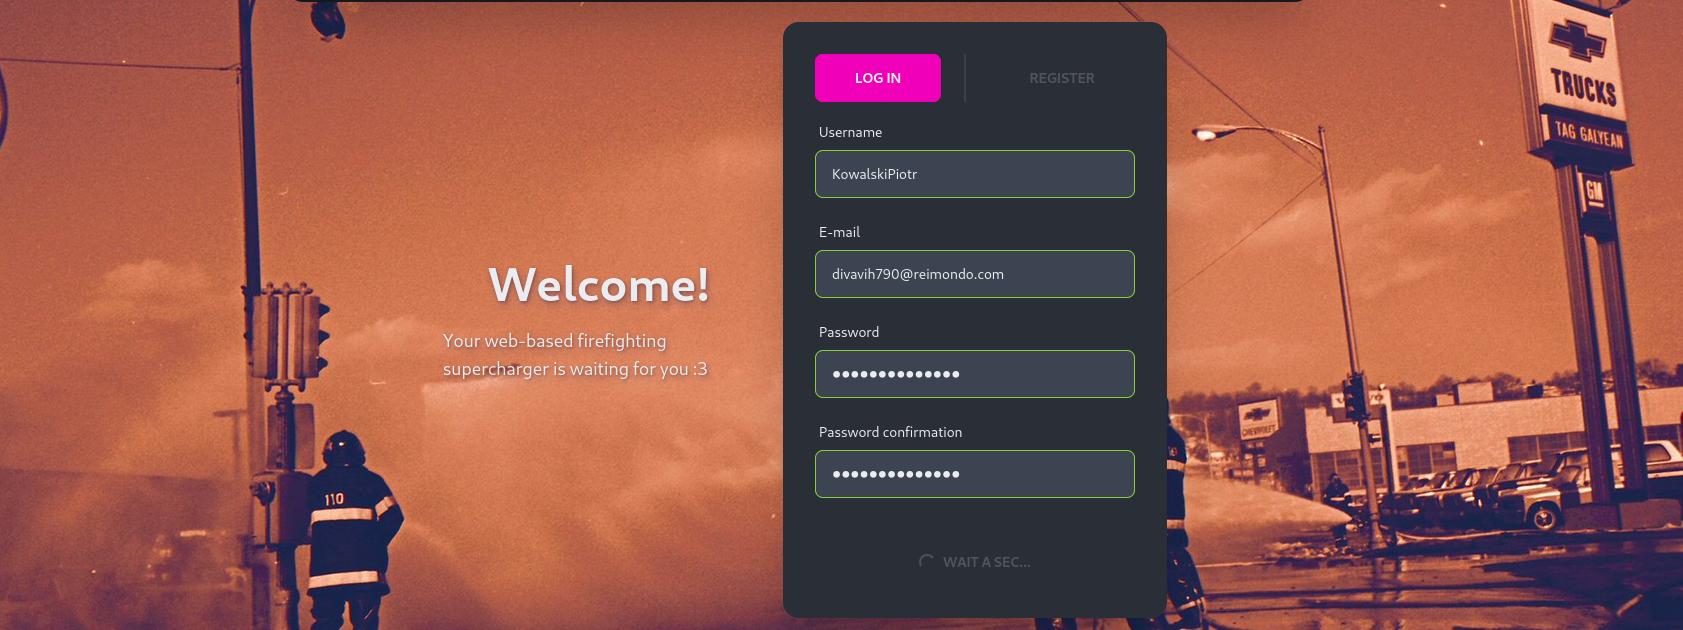
\includegraphics[width=\textwidth]{img/chapter5/registration.png}
\caption{Wypełniony formularz rejestracji, oczekujący na odpowiedź serwera}
\end{figure}

Proces rejestracji nowego użytkownika w systemie, rozpoczyna się od uzupełnienia jego danych w formularzu rejestracji i potwierdzenia ich przesłania. Formularz Razor wywołuje asynchroniczną metodę, przesyłającą żądanie "POST /api/users/register" do aplikacji serwerowej.

\begin{lstlisting}[language=CSharp, caption={Metoda kontrolera użytkowników odpowiedzialna za rejestrację nowego użytkownika w systemie}, label=lst:users_register]
[HttpPost("register")]
public async Task<ActionResult> Register([FromBody] UserRegisterDto dto) {
  try {
    if (TryValidateModel(dto) == false) {
      throw new ValidationProblemException();
    }
    var user = _mapper.MapRegister(dto);
    await _service.Create(user, dto.Password);
    var token = await _service.GetEmailConfirmationToken(user);
    var link = $"https://localhost:5001/verify/uid={user.Id}&token={token}";
    await _emailsService.SendVerificationEmail(user.Email, link);
    return Ok();
  }
  ...
}
\end{lstlisting}

Żądanie jest obsługiwane przez kontroler użytkowników, w metodzie Register() widocznej na listingu \ref{lst:users_register}. Za pomocą adnotacji FromBody, możliwe jest użycie ciała żądania jako argumentu metody. Po udanej walidacji danych formularza, jest on mapowany na nowy obiekt użytkownika i przekazywany wraz z łańcuchem hasła do metody serwisu, dedykowanej tworzeniu nowych użytkowników.

W przypadku powodzenia operacji, obiekt nowego użytkownika staje się mapowaną przez ORM reprezentacją encji. Z jego pomocą, generowany jest token potwierdzający adres e-mail, przesyłany następnie, na wskazany w procesie rejestracji adres, za pośrednictwem wstrzykniętego serwisu.

\begin{lstlisting}[language=CSharp, caption={Fragment serwisu mailowego aplikacji serwerowej}, label=lst:emailService]
public class EmailsService : IEmailsService {
  private readonly EmailSettings _emailSettings;

  public EmailsService(IOptions<EmailSettings> emailSettings) {
    _emailSettings = emailSettings.Value;
  }

  public async Task SendVerificationEmail(string email, string link) {
    var body = $@"
        ...
        <p>Please click <a href=""{link}"" target=""_blank"">this link</a> to confirm your email :)</p>
        ";
    await SendEmail(email, "OpenOSP Email Verification", body);
  }

  public async Task SendEmail(string email, string subject, string body) {
    using (var client = new SmtpClient()) {
      client.Host = _emailSettings.Server;
      ...
      await client.SendMailAsync(new MailMessage(_emailSettings.Address, email) {
        From = new MailAddress(_emailSettings.Address, _emailSettings.Name),
        Subject = subject,
        Body = body,
        IsBodyHtml = true,
        BodyEncoding = Encoding.UTF8
      });
    }
  }
}
\end{lstlisting}

Serwis e-mailowy aplikacji, pokazany na listingu \ref{lst:emailService}, korzysta z konfiguracji przekazanej z pliku appsettings.json, za pośrednictwem wstrzykniętej struktury EmailSettings. Obiekt klienta SMTP, stanowi przykład klasy wykorzystującej tzw. pamięć niezarządzalną, której zwalnianie przebiega za pośrednictwem interfejsu IDisposeable.

W bloku using, ograniczającym czas życia obiektu, tworzona jest konfiguracja klienta SMTP, umożliwiająca przesłanie wiadomości e-mail zawierającej w sobie link aktywacyjny. Celem zastosowania bloków i wyrażeń using, jest automatyczne wywoływanie metody Dispose(). W tym przypadku, służy ona poprawnemu zamknięciu połączenia z serwerem SMTP (przykład pamięci niezarządzalnej), po ukończeniu procedur wewnątrz bloku lub w sytuacji rzucenia wyjątku w jego wnętrzu.

% obraz otrzymanego maila
\begin{figure}[!htbp]
\centering
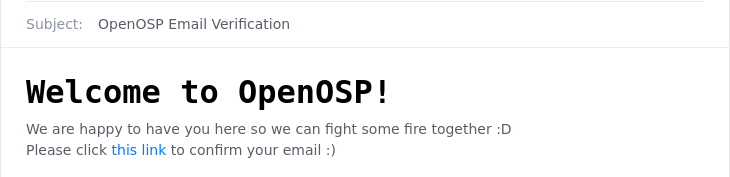
\includegraphics[width=\textwidth]{img/chapter5/email_content.png}
\caption{Wiadomość e-mail z linkiem potwierdzającym adres użytkownika}
\end{figure}

\begin{lstlisting}[language=CSharp, caption={Metoda kontrolera użytkowników, weryfikująca adres e-mail użytkownika}, label=lst:users_verify]
[HttpGet("verify")]
public async Task<ActionResult> Verify([FromQuery] int uid, [FromQuery] string token) {
  try {
    var user = await _service.ReadById(uid);
    await _service.ConfirmEmail(user, token);
    return Ok();
  }
  ...
}
\end{lstlisting}
 
Po przejściu na stronę wskazaną przez link aktywacyjny, komponent strony głównej, z listingu \ref{lst:razor_home}, wykorzystuje parametr przekazany przez URI, wysyłając żądanie obsługiwane przez metodę Verify() ukazaną na listingu \ref{lst:users_verify}. Identyfikator użytkownika oraz token potwierdzający, są przekazywane do argumentów metody, przy pomocy adnotacji FromQuery, odpowiedzialnej za obsługę tzw. zapytań URI.

% obraz strony głównej po kliknięciu w link aktywacyjny (lub sama belka potwierdzenia)
\begin{figure}[!htbp]
\centering

\includegraphics[width=\textwidth]{img/chapter5/confirmed.png}
\caption{Komunikat potwierdzenia adresu e-mail użytkownika}
\label{fig:confirmation}
\end{figure}

W przypadku udanej próby potwierdzenia adresu, na stronie głównej zostaje wyświetlony komunikat, widoczny na rys. \ref{fig:confirmation}. Komunikat znika po upływie 10 sekund, tak jak zostało to opisane pod listingiem \ref{lst:razor_home}.

%%%%%%%%%%%%%%%%%%%%%%%%%%%%%%%%%%%%%%%%%%%%%%%%%%%%%%%%%%%%%%%%%%%%%%%%%%%%%%%%
\subsection{Uwierzytelnianie i usuwanie danych uwierzytelniających}
%%%%%%%%%%%%%%%%%%%%%%%%%%%%%%%%%%%%%%%%%%%%%%%%%%%%%%%%%%%%%%%%%%%%%%%%%%%%%%%%

% obraz formularza logowania
\begin{figure}[!htbp]
\centering
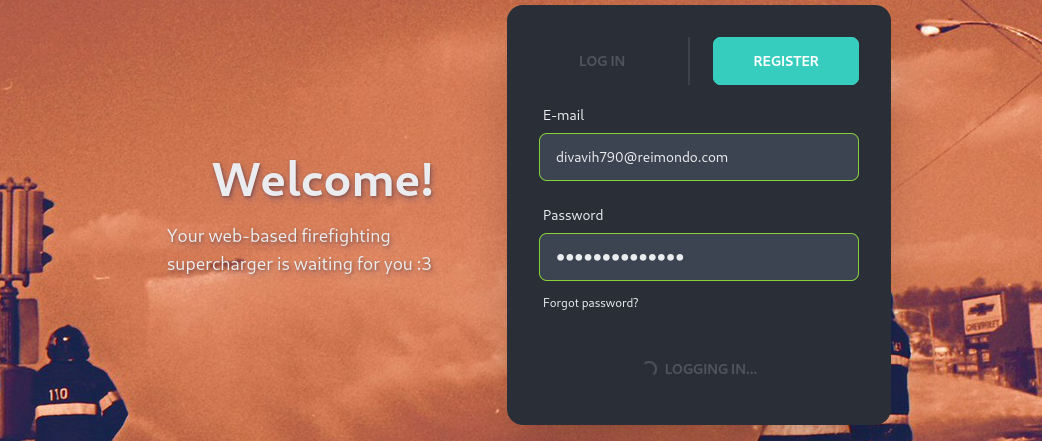
\includegraphics[width=\textwidth]{img/chapter5/login.png}
\caption{Wypełniony formularz logowania oczekujący na odpowiedź serwera}
\label{fig:form_login}
\end{figure}

Uwierzytelnianie użytkownika odbywa się poprzez formularz logowania widoczny na rys. \ref{fig:form_login}. Metoda obsługująca zdarzenie przesłania danych formularza, korzysta ze wstrzykniętego serwisu uwierzytelniania.

\begin{lstlisting}[language=CSharp, caption={Metoda uwierzytelniająca użytkownika, w klasie serwisu uwierzytelniającego aplikacji klienckiej}, label=lst:login_request]
public async Task<string> Login(UserLoginDto loginDto) {
  var authResult = await _http.PostAsJsonAsync("api/users/login", loginDto);
  var authContent = await authResult.Content.ReadAsStringAsync();
  if (authResult.IsSuccessStatusCode is false) {
    return null;
  }
  ...
}
\end{lstlisting}

\begin{lstlisting}[language=CSharp, caption={Metoda kontrolera użytkowników, obsługująca żądanie uwierzytelniające}, label=lst:users_login]
[HttpPost("login")]
public async Task<ActionResult<string>> Login([FromBody] UserLoginDto dto) {
  try {
    if (TryValidateModel(dto) == false) {
      throw new ValidationProblemException();
    }
    var user = await _service.ReadByEmail(dto.Email);
    var token = await _service.GetAuthenticationToken(user, dto.Password);
    return Ok(token);
  }
  ...
}
\end{lstlisting}

Ciało metody Login(), przedstawionej na listingu \ref{lst:login_request}, rozpoczyna się od przesłania żądania "POST /api/users/login", z danymi logowania w formacie JSON, przekazanym przez komponent. Żądanie, obsługiwane jest przez metodę kontrolera użytkowników, widoczną na listingu \ref{lst:users_login}. Przy pomocy encji użytkownika wyszukanej po adresie e-mail, wywoływana jest metoda serwisu użytkowników, generująca token uwierzytelniający.

\begin{lstlisting}[language=CSharp, caption={Metoda serwisu użytkowników, generująca tokeny uwierzytelniające}, label=lst:genToken]
public async Task<string> GetAuthenticationToken(T user, string password) {
  var signInResult = await _signInManager.CheckPasswordSignInAsync(user, password, false);
  if (signInResult.Succeeded == false) {
    throw new UnauthorizedException();
  }
  var claimsIdentity = new ClaimsIdentity(
    new[] {
      new(JwtRegisteredClaimNames.Jti, Guid.NewGuid().ToString()), 
      new Claim(JwtRegisteredClaimNames.Sub, user.Email),
      new Claim(JwtRegisteredClaimNames.UniqueName, user.Email), 
      new Claim("uid", user.Id.ToString())
    },
    "Token"
  );
  var key = new SymmetricSecurityKey(Encoding.UTF8.GetBytes(_jwtSettings.Key));
  var signingCredentials = new SigningCredentials(key, SecurityAlgorithms.HmacSha256);
  var token = new JwtSecurityToken(
    _jwtSettings.Issuer,
    _jwtSettings.Audience,
    claimsIdentity.Claims,
    expires: DateTime.UtcNow.AddDays(2),
    signingCredentials: signingCredentials
  );
  return new JwtSecurityTokenHandler().WriteToken(token);
}
\end{lstlisting}

Metoda na listingu \ref{lst:genToken}, rozpoczyna się od sprawdzenia czy podane hasło jest poprawne. Następnie zdefiniowane zostały twierdzenia, przesyłane w ładunku tokena: unikalny identyfikator tokena (jti), podmiot tokena (sub) oraz jego unikalne imię (unique\_name) zawierające w sobie adres e-mail użytkownika, wyświetlany na stronie, a na koniec klucz główny użytkownika, wykorzystywany w procesie autoryzacji per-wiersz.

Podczas tworzenia tokena, ponownie wykorzystuje się konfigurację widoczną na listingu \ref{lst:appsettings_jwt}. Emitent i odbiorca klucza, zostają dołączeni do tworzonego tokena, wraz z twierdzeniami, a sekretny klucz wykorzystywany jest w kontekście algorytmu podpisującego HMACSHA256. Dodatkowo, na token nakładany jest czas ważności, wynoszący dwa dni. Na etapie autoryzacji, sprawdzona zostaje zarówno autentyczność tokena jak i zgodność danych JWT, z zastosowaną na listingu \ref{lst:config_jwt} konfiguracją schematu.

\begin{lstlisting}[language=CSharp, caption={Fragment metody uwierzytelniającej użytkownika, zapisujący otrzymane dane uwierzytelniające pamięci}, label=lst:login_storage]
await _localStorage.SetItemAsync("authToken", authContent);
((AuthStateProvider) _authStateProvider).NotifyUserAuthentication(authContent);
_http.DefaultRequestHeaders.Authorization = new AuthenticationHeaderValue("bearer", authContent);
return authContent;
\end{lstlisting}

Po udanym utworzeniu i odebraniu uwierzytelniającego JWT w odpowiedzi HTTP, zostaje on zapisany w webowej pamięci lokalnej, w sposób pokazany na listingu \ref{lst:login_storage}. Wstrzyknięty do serwisu dostawca stanu uwierzytelnienia aplikacji Blazor, zostaje poinformowany o zalogowaniu użytkownika, za pośrednictwem metody rozszerzającej NotifyUserAuthentication(), opisanej poniżej. Na końcu, w kliencie HTTP, ustawiany jest nagłówek autoryzujący, ze schematem elementu niosącego dane, tak jak na listingu \ref{lst:jwt.authorization}.

\begin{lstlisting}[language=CSharp, caption={Metody klasy rozszerzającej dostawcę stanu uwierzytelnienia, w aplikacji klienckiej}, label=lst:authStateProvider_login]
public override async Task<AuthenticationState> GetAuthenticationStateAsync() {
  var token = await _localStorage.GetItemAsync<string>("authToken");
  if (string.IsNullOrEmpty(token)) {
    return _anonymous;
  }
  _httpClient.DefaultRequestHeaders.Authorization = new AuthenticationHeaderValue("bearer", token);
  return new AuthenticationState(
    new ClaimsPrincipal(
      new ClaimsIdentity(
        JwtParser.ParseClaimsFromJwt(token),
        "jwtAuthType")));
}

public void NotifyUserAuthentication(string token) {
  var authenticatedUser = new ClaimsPrincipal(
    new ClaimsIdentity(
      JwtParser.ParseClaimsFromJwt(token),
      "jwtAuthType"));
  var authState = Task.FromResult(new AuthenticationState(authenticatedUser));
  NotifyAuthenticationStateChanged(authState);
}
\end{lstlisting}

Metody rozszerzonego dostawcy stanu uwierzytelnienia, ukazane na listingu \ref{lst:authStateProvider_login}, dostosowują sposób jego działania do tokenów JWT, składowanych przy pomocy pamięci lokalnej. 

Nadpisana metoda GetAuthenticationStateAsync() jest wykorzystywana przez autoryzowane komponenty Razor, w celu pozyskania informacji o zalogowanym użytkowniku. Dodana NotifyUserAuthentication() ma na celu, natychmiastowe poinformowanie komponentów aplikacji, o zmianie stanu uwierzytelnienia oraz udostępnienie sparsowanego ładunku tokena, za pośrednictwem kontekstu aplikacji.

% obraz dropdownu z przyciskiem wylogowania
\begin{figure}[!htbp]
\centering

\includegraphics[width=\textwidth]{img/chapter5/sign_out.png}
\caption{Rozwijany element strony z przyciskiem usuwania danych uwierzytelniających użytkownika}
\label{fig:user_dropdown}
\end{figure}

Przykładem wykorzystania danych użytkownika, wpisanych wcześniej do kontekstu, jest rozwijany komponent na rys. \ref{fig:user_dropdown}. Zawiera w sobie również przycisk służący do wylogowywania użytkowników.

\begin{lstlisting}[language=CSharp, caption={Metoda obsługująca zdarzenie wylogowania użytkownika}, label=lst:logout]
public async Task Logout() {
  await _localStorage.RemoveItemAsync("authToken");
  ((AuthStateProvider)_authStateProvider).NotifyUserLogout();
  _http.DefaultRequestHeaders.Authorization = null;
}
\end{lstlisting}

\begin{lstlisting}[language=CSharp, caption={Metoda dostawcy stanu uwierzytelnienia odpowiedzialna za usunięcie danych uwierzytelniających}, label=lst:authStateProvider_logout]
public void NotifyUserLogout() {
  var authState = Task.FromResult(_anonymous);
  NotifyAuthenticationStateChanged(authState);
}
\end{lstlisting}

Wylogowanie użytkownika, polega na usunięciu utworzonego wcześniej w webowej pamięci lokalnej wartości tokena oraz poinformowaniu komponentów Razor, o zmianie stanu uwierzytelnienia, za pośrednictwem dostawcy. Na końcu, usuwany jest nieaktualny nagłówek Authorize z żądań HTTP.

%%%%%%%%%%%%%%%%%%%%%%%%%%%%%%%%%%%%%%%%%%%%%%%%%%%%%%%%%%%%%%%%%%%%%%%%%%%%%%%%
\subsection{Autoryzacja per-wiersz i w komponentach Razor}
%%%%%%%%%%%%%%%%%%%%%%%%%%%%%%%%%%%%%%%%%%%%%%%%%%%%%%%%%%%%%%%%%%%%%%%%%%%%%%%%

W poprzednich sekcjach, opisane zostały kwestie, związane z autoryzacją dostępu do punktów końcowych interfejsu REST. Jednakże, system wykorzystuje również mechanizm autoryzacji na poziomie zapytań do bazy danych, typu per-wiersz. Jej założeniem jest zastosowanie filtrów, umożliwiających dostęp do poszczególnych encji zasobu, jedynie użytkownikowi będącemu ich właścicielem (w relacji jeden-do-wielu), za pośrednictwem interfejsu IOwnedBy.

\begin{lstlisting}[language=CSharp, caption={Konfiguracja autoryzacji per-wiersz w bazie danych}, label=lst:dbContext_perRowProtection]
public class AppDbContext : IdentityUserContext<User, int> {
  private readonly int _userId;
  ...
  public AppDbContext(
    DbContextOptions<AppDbContext> options,
    IUserClaimsService<int> userClaims)
    : base(options) {
    _userId = userClaims.UserId;
  }
  ...
  protected override void OnModelCreating(ModelBuilder builder) {
    ...
    builder.Entity<Action>()
      .HasQueryFilter(e => e.UserId.Equals(_userId));
    builder.Entity<Equipment>()
      .HasQueryFilter(e => e.UserId.Equals(_userId));
    ...
  }

  public override async Task<int> SaveChangesAsync(CancellationToken cancellationToken = default) {
    var addedOwnedEntities = ChangeTracker.Entries()
      .Where(e => e.State.Equals(EntityState.Added) && e.Entity is IOwnedBy<int>)
      .Select(e => e.Entity as IOwnedBy<int>)
      .ToList();
    if (addedOwnedEntities.Count > 0 && _userId == default) {
      throw new UnauthorizedException();
    }
    addedOwnedEntities.ForEach(e => e.UserId = _userId);
    return await base.SaveChangesAsync(cancellationToken);
  }
}
\end{lstlisting}

\begin{lstlisting}[language=CSharp, caption={Serwis twierdzeń użytkownika, udostępniający klientom klucz główny uwierzytelnionego użytkownika}, label=lst:userClaimsService]
public class UserClaimsService<TId> : IUserClaimsService<TId>
  where TId : IEquatable<TId>, IComparable<TId>, IConvertible {
  public UserClaimsService(IHttpContextAccessor accessor) {
    var id = accessor.HttpContext?.User.Claims
      .SingleOrDefault(c => c.Type.Equals("uid"))?.Value;
    if (id == default) {
      return;
    }
    UserId = (TId)Convert.ChangeType(id, typeof(TId));
  }

  public TId UserId { get; }
}
\end{lstlisting}

Cała konfiguracja tego mechanizmu, znajduje się w klasie kontekstu bazy danych, który za pośrednictwem wstrzykiwanego serwisu twierdzeń użytkownika, jest w stanie porównywać klucz właściciela zasobu, z kluczem użytkownika, który utworzył obsługiwane żądanie HTTP. W metodzie OnModelCreating pokazane zostały dwa przykłady konfiguracji filtrów mechanizmu.

Nadpisana metoda SaveChangesAsync(), jest odpowiedzialna za automatyczne uzupełnienie atrybutu klucza właściciela, w nowo dodanych encjach, których klasy implementują interfejs IOwnedBy. 

W przypadku aplikacji klienckiej, autoryzacja komponentów oparta jest o kontekst aplikacji, wspomniany w poprzedniej podsekcji. Kontekst, zawiera w sobie informacje o obecnie zalogowanym użytkowniku, przekazane wcześniej przez dostawcę stanu uwierzytelnienia aplikacji, zarejestrowanego na listingu \ref{lst:blazor_auth}.

\begin{lstlisting}[language=CSharp, caption={Fragment głównego komponentu aplikacji klienckiej, odpowiadający za autoryzację widoków}, label=lst:authorizeRouteView]
<AuthorizeRouteView RouteData="@routeData" DefaultLayout="@typeof(Body)">
  <Authorizing>
    <div class="w-full h-full flex justify-center items-center bg-base-300">
      <button class="btn btn-primary btn-outline btn-lg loading">Authorizing...</button>
    </div>
  </Authorizing>
  <NotAuthorized>
    <OpenOsp.Client.Pages.Unauthorized/>
  </NotAuthorized>
</AuthorizeRouteView>
\end{lstlisting}

Autoryzacja widoków w aplikacji klienckiej, zostaje zapoczątkowana w komponencie głównym projektu, w którym użyto komponentu AuthorizeRouteView, odpowiedzialnego za renderowanie tylko tych komponentów-stron, do których przyznano dostęp użytkownikowi. Element Authorizing zawiera w sobie treść, która zostanie wyświetlona podczas sprawdzania uprawnień użytkownika, do wyświetlenia danego komponentu-strony. W przypadku odmowy dostępu do żądanej ścieżki, wyświetlony zostanie schemat zawarty w elemencie NotAuthorized.

\begin{lstlisting}[language=CSharp, caption={Zastosowanie adnotacji Authorize w komponentach Razor}, label=lst:razor_authorize]
@attribute [Authorize]
\end{lstlisting}

W celu autoryzacji całego komponentu, można zastosować adnotację Authorize, w sposób pokazany na listingu \ref{lst:razor_authorize}. Komponent będzie wyświetlany tylko dla tych użytkowników, którzy uwierzytelnili się w systemie.

\begin{lstlisting}[language=CSharp, caption={Blok widoku autoryzowanego AuthorizeView}, label=lst:razor_authorizeView]
<AuthorizeView>
  <Authorized>
    ...
  </Authorized>
  <NotAuthorized>
    ...
  </NotAuthorized>
</AuthorizeView>
\end{lstlisting}

Listing \ref{lst:razor_authorizeView} pokazuje bardziej elastyczne podejście, za pomocą którego, można określać części schematu podlegające autoryzacji. Blok AuthorizeView może zawierać w sobie trzy główne rodzaje elementów:

\begin{itemize}
    \item Authorized, wewnątrz którego, definiowany jest fragment schematu wyświetlany dla użytkownika uwierzytelnionego.
    \item NotAuthorized, określający treść wyświetlaną w przypadku użytkownika nieuwierzytelnionego.
    \item Authorizing - schemat wyświetlany przez blok w czasie procesu autoryzacji.
\end{itemize}

\begin{lstlisting}[language=CSharp, caption={Dostęp do stanu uwierzytelnienia wewnątrz bloku AuthorizeView>Authorize}, label=lst:razor_authContext]
<AuthorizeView>
  <Authorized>
    ...
      <li>
        <p class="font-bold select-none">@context.User.FindFirst(JwtRegisteredClaimNames.UniqueName).Value</p>
      </li>
    ...
  </Authorized>
</AuthorizeView
\end{lstlisting}

Dodatkową funkcjonalnością, posiadaną przez bloki komponentów autoryzacyjnych, jest łatwy dostęp do stanu uwierzytelnienia. Na listingu \ref{lst:razor_authContext}, pokazano fragment schematu, odpowiedzialny za wstawianie adresu e-mail użytkownika, w rozwijanym panelu ukazanym na rys. \ref{fig:user_dropdown}, korzystając z twierdzeń przekazanych do aplikacji w tokenie JWT.

Wszystkie mechanizmy autoryzacji, opisane w ramach tej podsekcji, zostały wykorzystane w systemie w podstawowej formie. Jednakże, w przypadku wprowadzenia np. ról lub grup użytkowników, rozszerzenie ich funkcjonalności o obsługę tych twierdzeń, nie wiązałoby się z dużo większym nakładem pracy, ze względu na dużą elastyczność tych rozwiązań.

\chapter{Podsumowanie}
%%%%%%%%%%%%%%%%%%%%%%%%%%%%%%%%%%%%%%%%%%%%%%%%%%%%%%%%%%%%%%%%%%%%%%%%%%%%%%%%
\section{Efekt końcowy}
%%%%%%%%%%%%%%%%%%%%%%%%%%%%%%%%%%%%%%%%%%%%%%%%%%%%%%%%%%%%%%%%%%%%%%%%%%%%%%%%

Efektem pracy jest system, zaimplementowany zgodnie z projektem, przedstawionym przy pomocy opisów i diagramów UML, spełniający wymagania postawione mu w rozdziale wprowadzającym pracy:

\begin{itemize}
    \item Aplikacja kliencka działa w przeglądarce internetowej, dlatego w odróżnieniu od rozwiązań istniejących na rynku, może zostać wykorzystana na wszystkich platformach posiadających to oprogramowanie, wliczając w to platformy mobilne.
    \item Aplikacja pojedynczej strony jest w pełni responsywna, dzięki zastosowanym arkuszom CSS.
    \item System korzysta z różnych rodzajów mechanizmów autoryzacji, zapewniających bezpieczeństwo danych użytkownika oraz wyświetlanie adekwatnych treści po stronie klienta.
    \item Aplikacja serwerowa wykorzystuje kilka warstw logicznych, luźno powiązanych ze sobą klas i wzorzec zastrzyków zależności, pozwalających na łatwą modyfikację i rozszerzenie projektu.
\end{itemize}

%%%%%%%%%%%%%%%%%%%%%%%%%%%%%%%%%%%%%%%%%%%%%%%%%%%%%%%%%%%%%%%%%%%%%%%%%%%%%%%%
\section{Dalszy rozwój aplikacji}
%%%%%%%%%%%%%%%%%%%%%%%%%%%%%%%%%%%%%%%%%%%%%%%%%%%%%%%%%%%%%%%%%%%%%%%%%%%%%%%%

W przypadku dalszego rozwoju aplikacji należałoby rozważyć następujące rozszerzenia:

\begin{itemize}
    \item Wprowadzenie ról użytkowników takich jak: administrator systemu oraz zarządca i członkowie jednostki, jako użytkownicy systemu, posiadający odrębne możliwości ułatwiające ich współpracę.
    \item Dodanie opcji generowania raportów i dokumentów do pobrania ze strony, przydatnych m.in. przy załatwianiu spraw urzędowych.
    \item Przyznawanie odznak i rang członkom jednostek, rozbudowujących ich uprawnienia w systemie.
    \item Rozbudowanie systemu o nowe moduły np. rozliczania czasu pracy.
    \item Przebudowanie systemu w sieć biznesową, łączącą wiele jednostek na mapie Polski, uwzględniając transfery sprzętu i członków zespołu między nimi.
\end{itemize}

%%%%%%%%%%%%%%%%%%%%%%%%%%%%%%%%%%%%%%%%%%%%%%%%%%%%%%%%%%%%%%%%%%%%%%%%%%%%%%%%
\section{Wnioski po ukończeniu pracy}
%%%%%%%%%%%%%%%%%%%%%%%%%%%%%%%%%%%%%%%%%%%%%%%%%%%%%%%%%%%%%%%%%%%%%%%%%%%%%%%%

W trakcie tworzenia pracy, jej początkowe założenia uległy kilku modyfikacjom, które wpłynęły na jej ostateczną formę i wartość merytoryczną. Początkowo, praca zakładała opisanie wprowadzania zmian w systemie, w kolejnych iteracjach projektu, we współpracy z użytkownikami.

Niestety, ze względu na obostrzenia wprowadzone w związku z sytuacją pandemiczną SARS-CoV-2, możliwości nawiązania bezpośredniej współpracy z jednostkami Ochotniczej Straży Pożarnej, zostały ograniczone. W związku z tym, w pracy kompleksowo przedstawiono założenia i sposób działania oraz rozwoju współczesnych systemów internetowych.

W ramach pracy wykorzystano, uporządkowano i rozwinięto wiedzę inżynierską, nabytą w trakcie trwania studiów, z wyszczególnieniem kursów:

\begin{itemize}
    \item Nowoczesne Technologie Internetowe - poświęconego tworzeniu aplikacji internetowych z użyciem pełnych stosów technologicznych.
    \item Inżynieria Oprogramowania - tworzącego wprowadzenie do tematu wzorców projektowych oraz metod dokumentowania projektów przy pomocy diagramów UML.
    \item Podstawy Sieci Komputerowych - dającego możliwość własnoręcznego wykorzystania protokołów tworzących sieć Internet.
\end{itemize}

Utworzenie prostego, lecz kompleksowego, rozwiązania biznesowego było dla autora okazją, do rewizji teoretycznej wiedzy o technologiach związanych z platformą internetową, wykorzystywaną w jego pracy zawodowej. Dodatkowo, praca umożliwiła przetestowanie eksperymentalnej platformy Blazor, mogącej wyznaczyć drogę dla nowej generacji platform aplikacji klienckich. 

Otwarta architektura Internetu, przyczyniła się do jego prężnego rozwoju w ostatnich dekadach. Bazując na ideach omawianych i standaryzowanych, przez inżynierów oprogramowania z całego świata, przeszedł drogę od niezawodnego sposobu przesyłania danych, do najpopularniejszej na świecie platformy, dostarczającej użytkownikom aplikacje wykorzystywane w ich codziennym życiu. Technologie internetowe zawdzięczają swoją obecną formę społeczności, w której udział poszczególnych twórców oprogramowania, ma wpływ na ich dalszy rozwój, skupiony na ciągłym doskonaleniu doświadczeń zarówno użytkowników, jak i twórców systemów. %ufff


%\appendix
%\chapter{Acronyms and Symbols}
%Lorem ipsum dolor sit amet, consectetur adipiscing elit. Donec faucibus diam at nibh ultrices, vel consectetur massa facilisis. Morbi et magna fermentum, rhoncus metus ut, pulvinar purus. Quisque at purus quis arcu finibus euismod eu quis lacus. Nulla pretium eu dui vel facilisis. Etiam vestibulum eu ex vel lobortis. Aliquam tincidunt nunc velit, auctor molestie nulla vehicula vitae. Pellentesque habitant morbi tristique senectus et netus et malesuada fames ac turpis egestas. Donec convallis ligula eget tortor blandit, ac molestie ex vulputate.

Nunc vitae arcu sit amet tellus accumsan molestie non a diam. Fusce ut purus quis tortor auctor venenatis. Donec sit amet felis eu dui mattis rhoncus vitae id lorem. Nunc id luctus sapien, id semper lectus. Etiam elit odio, faucibus molestie semper sit amet, sodales sit amet mi. In lobortis odio sit amet nulla malesuada imperdiet. Duis aliquam mauris nec rutrum sodales. In ullamcorper magna volutpat neque iaculis consequat. Fusce sit amet eros sit amet augue suscipit pulvinar. Donec non nunc augue. In varius est eget quam finibus bibendum. Etiam sed aliquet dolor. Vestibulum iaculis commodo venenatis. Mauris ut sapien diam. Sed ultrices nisi justo, et efficitur tellus lobortis non.

Pellentesque porttitor, arcu ac consectetur consequat, sem nisi rhoncus nibh, vel rutrum eros nibh eget mauris. Aliquam ac dui in ligula auctor finibus. Sed sed laoreet mi, sed accumsan orci. Morbi feugiat odio sit amet magna placerat cursus. Interdum et malesuada fames ac ante ipsum primis in faucibus. Maecenas venenatis velit sed dui tincidunt, sit amet luctus sem rhoncus. Mauris eros enim, iaculis et gravida ut, sagittis et eros.

\newpage
\listoffigures

\newpage
\listoftables

\newpage
\addcontentsline{toc}{chapter}{Spis listingów}
\lstlistoflistings

\printbibliography[heading=bibintoc]

\end{document}